% THIS IS AN EXAMPLE DOCUMENT FOR VLDB 2012
% based on ACM SIGPROC-SP.TEX VERSION 2.7
% Modified by  Gerald Weber <gerald@cs.auckland.ac.nz>
% Removed the requirement to include *bbl file in here. (AhmetSacan, Sep2012)
% Fixed the equation on page 3 to prevent line overflow. (AhmetSacan, Sep2012)
%\newcommand{\sigmod} %% Uncomment this line to enable formatting for SIGMOD
\newcommand{\vldb} %% Uncomment this line to enable formatting for VLDB.

\newcommand{\cameraready} %% Uncomment this line to enable formatting for camera-ready version.

\ifdefined\sigmod
\documentclass[sigconf]{acmart}
% Copyright
%\setcopyright{none}
%\setcopyright{acmcopyright}
%\setcopyright{acmlicensed}
\setcopyright{rightsretained}
%\setcopyright{usgov}
%\setcopyright{usgovmixed}
%\setcopyright{cagov}
%\setcopyright{cagovmixed}


% DOI
\acmDOI{10.475/123_4}

% ISBN
\acmISBN{123-4567-24-567/08/06}

%Conference
\acmConference[SIGMOD'18]{ACM SIGMOD conference}{June 2018}{Houston, Texas USA}
\acmYear{2018}
\copyrightyear{2016}


\acmArticle{4}
\acmPrice{15.00}

\else
\documentclass{vldb}
\fi
%\documentclass{sig-alternate}

%\newcommand{\submit} %% Uncomment this command before the final submission for review.

%\newcommand{\anonymized} %% Uncomment this command if submitting to a double-bling conference.

%\newcommand{\cameraready} %% Uncomment this command before final camera ready submission.

\ifdefined\sigmod
\unless\ifdefined\cameraready
\newcommand{\anonymized}
\fi
\fi

\ifdefined\cameraready
\ifdefined\anonymized
\let\anonymized\undefined
\fi
\unless\ifdefined\submit
\newcommand{\submit}
\fi
\fi

\ifdefined\submit
\newcommand{\todo}[1]{}
\newcommand{\changed}[1]{#1}
\long\def\tocut#1{}
\else
\newcommand{\todo}[1]{\textcolor{red}{\bf [TODO!: #1]}}
%\newcommand{\changed}[1]{{\color{blue}#1}}
\newcommand{\changed}[1]{{#1}}
\newcommand{\tocut}[1]{\textcolor{red}{\it\st{#1}}}
\fi

\newcommand{\papertitle}{Improving Optimistic Concurrency Control Through Transaction Batching and Operation Reordering}

\ifdefined\vldb
% Include information below and uncomment for camera ready
\vldbTitle{\papertitle}
\vldbAuthors{Bailu Ding, Lucja Kot, Johannes Gehrke}
\vldbDOI{https://doi.org/10.14778/3282495.3282502}
\vldbVolume{12}
\vldbNumber{2}
\vldbYear{2018}
\fi

\usepackage[labelfont=bf]{caption} % Use bold for caption ID.

\usepackage{graphicx}
\usepackage{balance}  % for  \balance command ON LAST PAGE  (only there!)

\usepackage[linesnumbered]{algorithm2e}
\usepackage{caption}
\usepackage{subcaption}
\captionsetup[subfigure]{labelformat = parens, labelsep = space, font = small}
\usepackage{enumitem}

\usepackage[all]{nowidow} % prevent orphan and widow lines

%\usepackage{algorithm}
%\usepackage{algpseudocode}

% To get colored comments
\usepackage{color}  
\newcommand{\johannes}[1]{{\color{blue} Johannes: [{#1}]}}
\newcommand{\lucja}[1]{{\color{red} Lucja: [{#1}]}}
\newcommand{\bailu}[1]{{\color{red} Bailu: [{#1}]}}

\newcommand{\eat}[1]{} % comment out blocks of text
\newcommand{\cut}[1]{} % comment out blocks of text


\begin{document}

% ****************** TITLE ****************************************

%\title{Improving Optimistic Concurrency Control Through \\
%	Transaction Batching and Operation Reordering}
\title{\papertitle}

% possible, but not really needed or used for PVLDB:
%\subtitle{[Extended Abstract]
%\titlenote{A full version of this paper is available as\textit{Author's Guide to Preparing ACM SIG Proceedings Using \LaTeX$2_\epsilon$\ and BibTeX} at \texttt{www.acm.org/eaddress.htm}}}

% ****************** AUTHORS **************************************

% You need the command \numberofauthors to handle the 'placement
% and alignment' of the authors beneath the title.
%
% For aesthetic reasons, we recommend 'three authors at a time'
% i.e. three 'name/affiliation blocks' be placed beneath the title.
%
% NOTE: You are NOT restricted in how many 'rows' of
% "name/affiliations" may appear. We just ask that you restrict
% the number of 'columns' to three.
%
% Because of the available 'opening page real-estate'
% we ask you to refrain from putting more than six authors
% (two rows with three columns) beneath the article title.
% More than six makes the first-page appear very cluttered indeed.
%
% Use the \alignauthor commands to handle the names
% and affiliations for an 'aesthetic maximum' of six authors.
% Add names, affiliations, addresses for
% the seventh etc. author(s) as the argument for the
% \additionalauthors command.
% These 'additional authors' will be output/set for you
% without further effort on your part as the last section in
% the body of your article BEFORE References or any Appendices.

\numberofauthors{3}

\author{
% You can go ahead and credit any number of authors here,
% e.g. one 'row of three' or two rows (consisting of one row of three
% and a second row of one, two or three).
%
% The command \alignauthor (no curly braces needed) should
% precede each author name, affiliation/snail-mail address and
% e-mail address. Additionally, tag each line of
% affiliation/address with \affaddr, and tag the
% e-mail address with \email.
%
% 1st. author
\alignauthor Bailu Ding \\
	%\affaddr{Cornell University, Microsoft Research}\\
    \affaddr{Microsoft Research}\\
    \email{badin@microsoft.com}
% 2nd. author
\alignauthor Lucja Kot\titlenote{Work performed while at Cornell University.} \\
	\affaddr{GrammaTech, Inc}\\
    \email{lkot@grammatech.com}
\and
\alignauthor Johannes Gehrke\\
	\affaddr{Microsoft Corporation}\\
    \email{johannes@microsoft.com}
}

\maketitle

\begin{abstract}
	OLTP systems can often improve throughput by \emph{batching} transactions and processing them as a group. Batching has been used for optimizations such as message packing and group commits; however, there is little research on the benefits of a holistic approach to batching across a transaction's entire life cycle.
	
In this paper, we present an OLTP system based on optimistic concurrency control that incorporates batching at multiple stages of transaction execution. 
%Execution batching enables enables reordering of operations to improve performance and reduce conflicts: 
Storage batching enables reordering of transaction reads and writes at the storage layer, reducing \changed{conflicts on the same object}. Validator batching enables reordering of transactions before validation, reducing conflicts between transactions. Dependencies between transactions make transaction reordering a non-trivial problem, and we propose several efficient and practical algorithms that can be customized to various transaction precedence policies such as reducing tail latency. \changed{We also show how to parallelize validator batching for better performance, and how to assign transactions to threads for systems without a centralized validator.

In-depth experiments on a research prototype, an open-source OLTP system, and a production OLTP system show that our techniques can  more than triple system throughput and reduce average latency and tail latency by over 80\%.
} 
\end{abstract}

\section{Introduction}\label{sec:intro}

% batching is important
Transaction processing is a fundamental aspect of database functionality, and improving OLTP system performance has long been a key research goal in our community. It is well-known that the throughput of OLTP systems can be increased through \emph{batching}-based optimizations, whereby some component buffers a number of transactions or requests as they arrive and processes them as a group.

% batching for obvious reason: low level
Batching can improve system performance for several obvious reasons. First, it increases the efficiency of communication by packing messages~\cite{ding2015centiman,friedman1997packing}. Second, it amortizes the cost of system calls by condensing multiple requests into a single one, as in group commit~\cite{debrabant2013anti,hagmann1987reimplementing}. Third, it reduces the number of requests by discarding duplicate or stale ones, such as writes to the same record~\cite{faleiro2014lazy}. However, all of those are local optimizations based on low-level techniques.

% our proposal at a high level: batching at higher level for OCC 
We propose an OLTP system design that embraces batching as a core design principle at multiple stages of a transaction's execution. In particular, we explore the benefits of batching in optimistic concurrency control (OCC) to reduce conflicts~\cite{kung81tods}, and thus improve both system-wide and individual transaction performance. OCC is a popular concurrency control protocol due to its low overhead in low-contention settings~\cite{adya97podc, baker11cidr, bernstein2015optimizing,bernstein11cidr, bernstein11vldb, corbett12osdi,warp, patterson12vldb,peng10osdi}. However, it wastes resources when conflicts are frequent~\cite{agrawal1987concurrency}. We show how batching reduces the number of conflicts and extends the applicability of OCC to higher-contention workloads.


Figure~\ref{fig:occ_arch} shows a distributed OCC-based transaction processing system with centralized validation. The system consists of three components: processors, storage nodes, and a single validator. External clients issue transactions to the system. On arrival into the system, each transaction is assigned to a processor and enters its \emph{read} phase. The processor sends read requests to the storage, executes the transaction, and performs ``writes'' to a local workspace. After it has processed the transaction, it sends information about the transaction's reads and writes to the validator. 

The transaction now enters the \emph{validation} phase. In OCC with \emph{backward validation}, the validator checks whether the transaction conflicts with any previously committed transactions, and makes a ``success'' or ``failure'' validation decision. One example of a conflict that would cause validation to fail is a \emph{stale read}. Suppose a transaction $t$ reads an object, and a second transaction $t'$ writes to the same object after $t$'s read. If $t'$ commits before $t$, $t$ has a conflict, since it should have read the update $t'$ made to the object but it did not. Thus $t$ must fail validation. 


If a transaction passes validation, the processor sends its writes to the storage; this is the \emph{write} phase. Otherwise, the processor aborts and restarts the transaction.

% why OCC for batching
The architecture of OCC with backward validation presents unique opportunities for batching because transactions are only serialized prior to commit. 
% batching at processor
There are three obvious times and locations to apply batching. The first is the processor in the transactions' \emph{read} phase, where transaction requests can be batched before execution. There is recent work in the context of locking-based protocols that  batches transactions and serializes them before execution to reduce overheads~\cite{faleiro2014rethinking,mu2014extracting,thomson2012calvin}; these techniques could be adapted and applied in OCC as well.

% batching at validator
The second place we can batch is the validator, for transactions in the \emph{validation} phase. If the validator buffers the validation requests as they arrive, it has the flexibility to choose a validation order. This allows the validator to reduce the number of conflicts and aborts. Recall our previous example of a validation failure. A transaction $t$ reads an object, and a second transaction $t'$ writes to the same object after $t$'s read. If $t'$ arrives at the validator before $t$ and commits, $t$ must fail since it should have read the value written by $t'$ but it didn't. Instead, with batching, if transactions $t$ and $t'$ are both in the same batch waiting for validation, we can choose to serialize $t$ before $t'$. Thus, we avoid conflicts and both transactions can commit.

% batching at storage
Third, the system can perform batching at the storage level. This affects already-validated transactions in their \emph{write} phase as well as transactions still in their \emph{read} phase. The storage can buffer read and write requests into batches as they arrive. If a batch contains multiple read and write requests for the same object, the system can apply all the writes first, in the serialization order. Next, it can process the reads. Prioritizing writes over reads is always optimal in the sense that it reduces the number of aborts as much as possible. This is because OCC reads come from uncommitted transactions, while writes come from validated transactions that will commit soon. Thus if the storage has both a pending read and a pending write on the same object, but schedules the read before the write, the reading transaction will see a stale value and is guaranteed to fail validation. 

% drawback of batching
Batching at these three levels in the system reduces aborts due to conflicts, and thus can increase throughput.\eat{However, it may also increase latency.}

\begin{figure}[t]
 \centering
 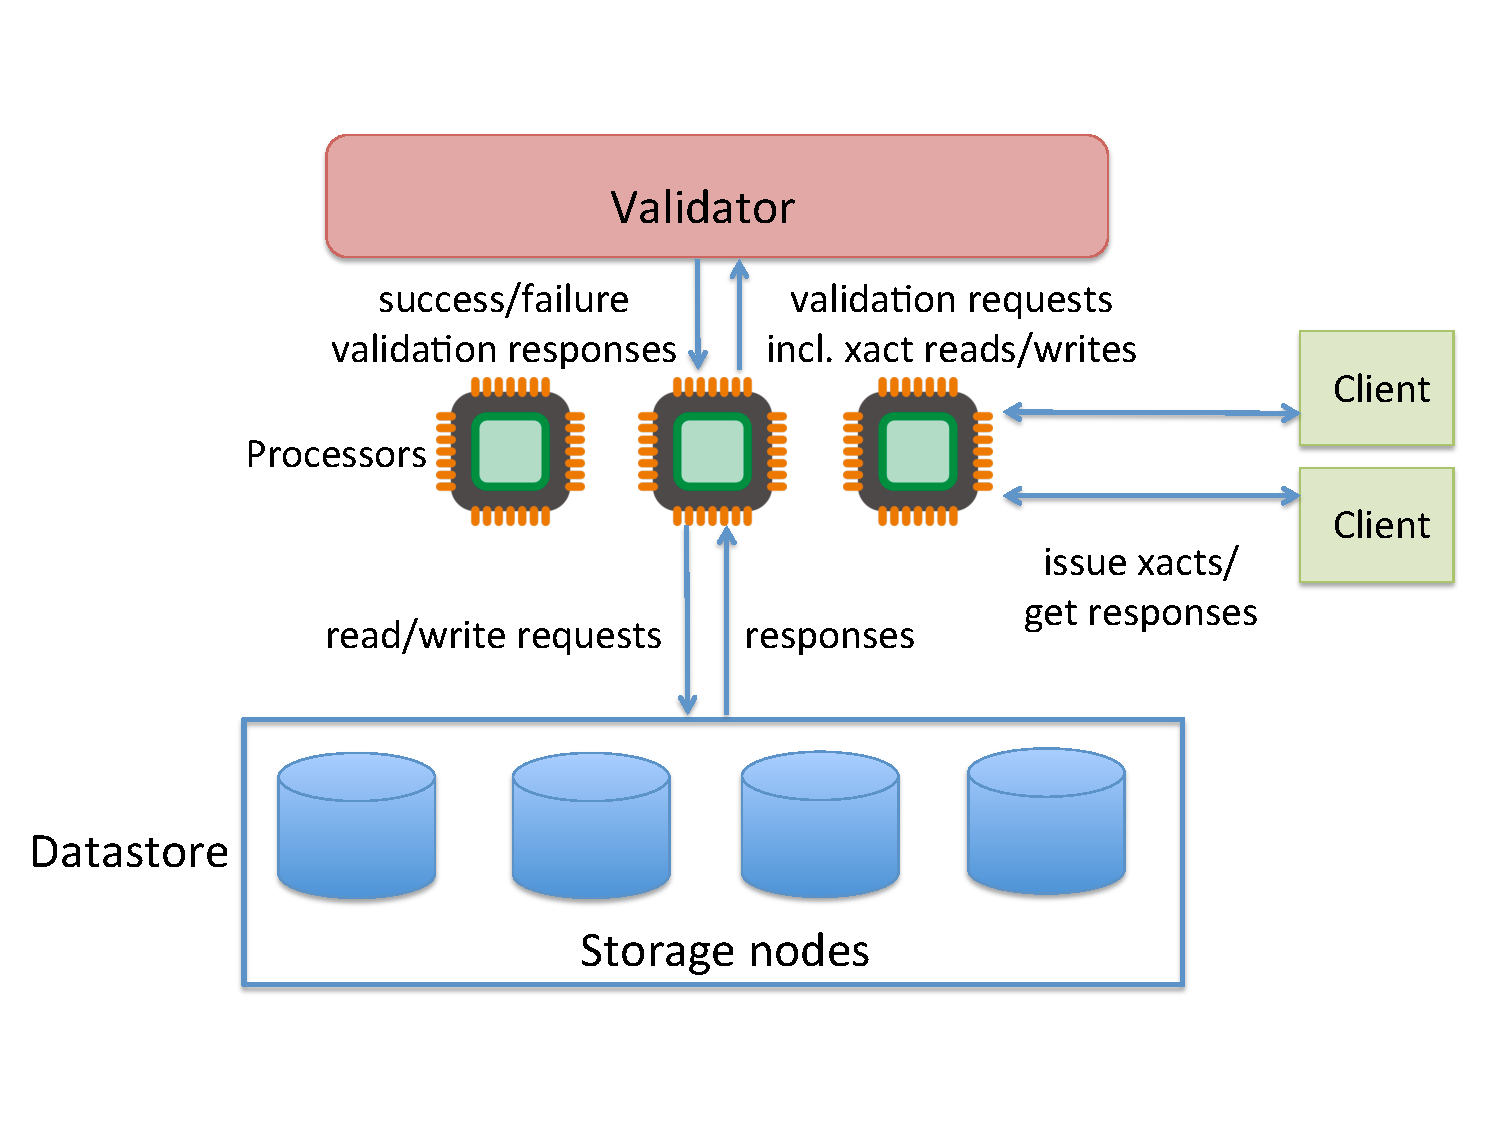
\includegraphics[width=0.7\columnwidth]{figures/OCCArchitecture.pdf}
 \vspace{-.5em}
 \caption{OCC System Architecture}
 \vspace{-1.5em}
 \label{fig:occ_arch}
\end{figure}


% contribution
In this paper, we explore in-depth the benefits of transaction batching in OCC with backward validation. Since there is substantial existing work that applies directly to processor batching, we focus on storage and validator batching, which have received little research interest so far.

% contribution 1: system design
Our first contribution is an enhanced OCC system architecture that includes batching at the storage and the validator levels. We analyze the reasons for conflicts and aborts at each stage of a transaction's life cycle, and develop techniques to reduce these aborts through batching and operation reordering.

% contribution 2: validator reordering algorithms
Our algorithmic focus is on validator batching, and specifically on reordering within a batch at the validator. Optimal transaction reordering within a validator batch is NP-complete, as it can be formulated as the problem of finding a minimal feedback vertex set in a directed graph~\cite{karp1972reducibility}. Our second contribution consists of two classes of greedy algorithms. These algorithms produce feedback vertex sets that are a close approximation to the optimal solution, and they are fast enough to be used in practice. 


Since the overhead of validator reordering increases transaction latency, it may hurt the end-to-end throughput of the system even it reduces the number of aborts. Our two classes of greedy algorithms explore this trade-off. Additionally, we extend our algorithms to weighted versions that can incorporate features such as transaction priorities.


\eat{
As mentioned before, the overhead of validator reordering increases transaction latency. Thus, even as validator reordering reduces the number of conflicts, it may hurt the end-to-end throughput of the system. Our two classes of greedy algorithms explore this trade-off. Additionally, we extend our algorithms to weighted versions that can incorporate features such as transaction priorities.
}

% contribution 3: experiment
Our third contribution is a detailed experimental study of the impacts of storage and validator batching on transaction execution performance. 
Our results show that batching always increases throughput and, surprisingly, also reduces transaction latency. When the workload has high data contention, batching and reordering can improve the throughput by up to 2.4x and reduce the average transaction latency by up to 21\% for both micro benchmarks and the Small Bank Benchmark~\cite{alomari2008icde}.

\eat{
% paper organization
The remainder of the paper is organized as follows. In Section~\ref{sec:background}  we review OCC with backward validation. In Section~\ref{sec:overview} we discuss challenges, opportunities and techniques for storage and validator batching. In Section~\ref{sec:validator_reordering}, we introduce our algorithms for intra-batch transaction reordering at the validator. In Section~\ref{sec:experiments}, we present an extensive experimental study of batching in our system. We discuss related work in Section~\ref{sec:relwork} and conclude in Section~\ref{sec:conclusion}.
}

\section{OCC Background}\label{sec:background}

% backward occ
In this paper, we use the term ``optimistic concurrency control'' to refer to the classical backward validation based protocol introduced in~\cite{kung81tods}. As explained in the introduction, this is a protocol where every transaction goes through three execution phases. First comes a \emph{read} phase, where the transaction reads data from the storage and executes while making writes to a private ``scratch workspace''. Then the transaction enters a \emph{validation} phase. If validation is successful, the transaction enters the \emph{write} phase, when its writes are installed in the storage. 

% details for validation
OCC validation enforces serializability; we only allow a transaction to pass validation if it can be serialized after all transactions that have already committed. The validator assigns each transaction a number (timestamp) and ensures that transactions are serialized in timestamp order.

To validate a transaction, we need to examine its reads and writes, and compare them to the writes of previously committed transactions. For a given transaction, we call the set of objects it has read its \emph{read set} and the set of objects it has written its \emph{write set}. When a transaction enters validation, its read set and write set are known, as are write sets of all previously committed transactions. For a transaction with timestamp $i$, we denote its read set by $RS(i)$ and its write set by $WS(i)$.

% the scope of validation
When validating a transaction with timestamp $j$ (transaction $T(j)$), the validator needs to check for conflicts with any transaction with timestamp $i$ (transaction $T(i)$) that have already committed (so $i < j$) and that overlapped temporally with $T(j)$, i.e. $T(i)$ hadn't committed when $T(j)$ started. 
% criterion for conflicts
$T(j)$ can be serialized after such a transaction $T(i)$ if one of the following conditions holds:
\begin{itemize}
\item $T(i)$ completed its write phase before $T(j)$ started its write phase, and $WS(i) \cap RS(j) = \emptyset$, or
\item $T(i)$ completed its read phase before $T(j)$ started its write phase, and $WS(i) \cap RS(j) = \emptyset$ as well as $WS(i) \cap WS(j) = \emptyset$
\end{itemize}

If $T(i)$ and $T(j)$ overlap temporally, and $WS(i) \cap RS(j) \neq \emptyset$, we say there is a \emph{read-write dependency} from $T(j)$ to $T(i)$. Intuitively, if there is such a dependency, $T(j)$ cannot be serialized after $T(i)$. In addition, we must ensure the writes of the two transactions are installed in the correct order to maintain consistency in the storage. If they write to the same object, the updates must be applied in their serialization order. The original OCC~\cite{kung81tods} algorithms achieve this by putting the validation and write phases in a critical section.

The batching techniques we study in this paper are applicable to most OCC systems; however, we make certain assumptions about the implementation of OCC validation, for simplicity and concreteness of our experimental setup. We clarify those assumptions now.

Given that our architecture (Figure~\ref{fig:occ_arch}) has a single validator, we assume the validation phase is sequential. We do not require the write phase to be in a critical section; this means that write requests may arrive at the storage out of order. We deal with this using a \emph{versioned} datastore; every item in the datastore is versioned and every write request is tagged with a version number equal to the writing transaction's timestamp. If the datastore receives a write request with version (timestamp) $i$ and a higher-numbered version $j > i$ already exists for the object, the write request is ignored. 

The above discussion implies that validation only needs to check, for every transaction $T(j)$ and all transactions $T(i)$ overlapping temporally with $T(j)$, where $i<j$, that $WS(i) \cap RS(j) = \emptyset$. Data versioning provides an easy way to determine whether $T(j)$ overlapped temporally with $T(i)$; every time a transaction performs a read, we tag the read with the version of the item that was read. If $T(j)$'s read set contains an item $X$ and the read saw version $k$, the validator only needs to check the write sets of all $T(i)$ with $k < i < j$ to see whether they contain $X$. This use of versioning in validation is identical to the one described in~\cite{ding2015centiman}.

%\section{Batching Overview}\label{sec:overview}

In this section, we explain how we can perform batching at the storage and the validator in an OCC system. 

\emph{Batching} involves buffering a number of requests as they arrive at some component of the system and processing them as a group. The goal of batching is to reduce the number of conflicts by reordering the operations in each batch, thus increasing the throughput. As explained in Section~\ref{sec:background}, aborts happen due to read-write dependencies involving a committed transaction $T(i)$ that wrote to some object, and a later transaction $T(j)$ that read the same object but did not see $T(i)$'s update. If $T(i)$ and $T(j)$ are in the same batch at the validator, we call this an \emph{intra-batch} abort of $T(j)$; if they are in a different batch, we call it an \emph{inter-batch} abort.

The server components -- the storage and the validator -- aim to reduce both intra-batch and inter-batch aborts. The storage batches the read and write requests, and the validator batches the validation requests.

Once a batch is fixed, the number of intra-batch aborts is determined by the amount of data contention among the requests in the batch and by the way we order and interleave the requests in processing. Thus the main optimization strategy is \emph{reordering}. The storage manager reduces aborts by reordering individual read and write operations, while the validator reduces aborts by changing the serialization order of transactions. The overhead of the reordering impacts transaction latency, so the reordering algorithms must be as fast as possible.

To reduce the number of inter-batch aborts, the system can divide the transactions into batches in a careful manner; it can also privilege writes over reads to allow reads to see fresher values. However, at all times in the system, there are multiple batches in-flight. No component can thus eliminate inter-batch aborts completely and unilaterally. The worst case is a slow transaction that writes an object and passes validation, but whose write gets ``stuck'' in the system and doesn't make it to the storage for a long time. This transaction will conflict with -- and cause inter-batch aborts of -- all subsequent transactions that read the same item, until the write is actually applied.

We now explain the specific batching strategies that are available at the storage and the validator.

\subsection{Storage Batching}
At the storage layer, the optimal batching strategy is simple. We buffer a certain number of read and write requests into batches. When a batch is ready, either when there are enough requests or a timeout is reached, for each object we apply the highest-version write request on that object. It is safe to discard all other writes on that object, as explained in Section~\ref{sec:background}. Next, we handle all the read requests for the same object. 

This strategy is optimal for reducing intra-batch aborts, as it ensures that all available writes by committed transactions are applied to all objects before we handle any read requests on these objects. The only way to reduce inter-batch aborts is to increase the batch size.

\subsection{Validator Batching}\label{subsec:overview:validator}

The validator buffers and batches transaction validation requests as they arrive. The optimal strategy for reducing inter-batch aborts is to ensure that transactions accessing the same objects are always batched together, that is, to cluster them based on access patterns.  Otherwise, the validator cannot do anything about conflicting transactions that are ``spread out'' across batches. There has been a lot of research on data clustering either online or offline~\cite{pavlo2012skew, elmore2015squall}, especially for fine-grained data partitioning. Any of these techniques can be used for validator batch creation. Of course, clustering transactions into batches based on access patterns may increase the number of intra-batch aborts.

Once the batches are fixed, the validator can reduce intra-batch aborts by choosing a good validation (i.e., serialization) order. The validator may not be able to eliminate all intra-batch aborts, since it cannot actually delay the execution of a transaction. Rather, it is presented with read and write sets of transactions that have already run. 

Intra-batch transaction reordering can be done with several goals in mind. We can simply minimize intra-batch aborts, i.e. maximize the number of transactions in each batch that commit. However, we may also want to prioritize certain transactions to have a greater chance of committing. For example, if we want to reduce the number of aborts \emph{per transaction}, we can increase a transaction's priority every time it has to abort and restart. Priorities could also be related to external factors (e.g. a transaction's monetary value or its chance of committing). These choices suggest a range of possible policies; we explore them in the next section.


%\section{Validator Reordering}\label{sec:validator_reordering}

In this section we present our algorithms for intra-batch validator reordering of transactions (IBVR). We formalize the problem and express it as an instance of the feedback vertex set (FVS) problem (Section~\ref{sec:ibvr}). We give two greedy algorithms for finding feedback vertex sets in Section~\ref{subsec:validator_reordering:algorithm} and show an example of executing these algorithms on a graph in Section~\ref{subsec:alg_example}. Both algorithms are parameterized on \emph{policies} that allow the validator to privilege certain transactions for committing; we discuss policies in Section~\ref{subsec:validator_reordering:policy}.

\subsection{Intra-Batch Validator Reordering (IBVR)}\label{sec:ibvr}

A \emph{batch} $B$ is a set of transactions to be validated. We assume all transactions $t \in B$ are \emph{viable}, that is, no $t \in B$ has a read-write dependency to a committed transaction. If there are non-viable transactions in $B$, they can be removed in preprocessing, as they must always abort.

\eat{
Given $B$, the goal of IBVR is to find a $B' \subseteq B$ of transactions that must abort due to intra-batch aborts. IBVR must also find a strict (i.e. asymmetric) total order $\prec$ on $B \setminus B'$ that \emph{respects all read-write dependencies}; that is, for $t,t'\in B \setminus B'$, if $t \prec t'$, then there is no read-write dependency from $t'$ to $t$.

The idea is that the validator processes each batch by running IBVR to identify $B'$ and $\prec$, aborting all the transactions in $B'$  and validating the transaction in $B \setminus B'$  in the order $\prec$. By the constraint we gave on $\prec$ above, and from the discussion in Section~\ref{sec:background}, $\prec$ is guaranteed to be a valid serialization order that allows all transactions in $B \setminus B'$  to commit.

There is always a trivial solution to any IBVR instance: we can choose $B'$ to be all the elements of $B$ except one, so that $B \setminus B'$ has cardinality one. Such solutions are not useful; therefore, every instance of IBVR is associated with an \emph{objective function} on $B'$, and the goal is to find a $B'$ that maximizes the objective function. An example objective function could be the size of $B'$ (smaller is better), or a more complex function that takes into account transaction weights (e.g. priorities).

}


Given $B$, the goal of IBVR is to find a $B' \subseteq B$ of transactions that must abort due to intra-batch aborts, and a commit order $Q$ for the remaining transactions that respects all read-write dependencies.

The validator processes each batch by running IBVR to identify $B'$ and $Q$, aborting all the transactions in $B'$ and committing remaining transactions in the order of $Q$.

There is always a trivial solution to any IBVR instance: aborting every transaction but one. Such solutions are not useful; therefore, every instance of IBVR is associated with an \emph{objective function} on $B'$, and the goal is to find a $B'$ that maximizes the objective function. An example objective function could be the size of $B'$ (smaller is better), or a more complex function that takes into account transaction weights (e.g. priorities).

\subsubsection{IBVR using feedback vertex set}

\begin{figure}[t]
\centering
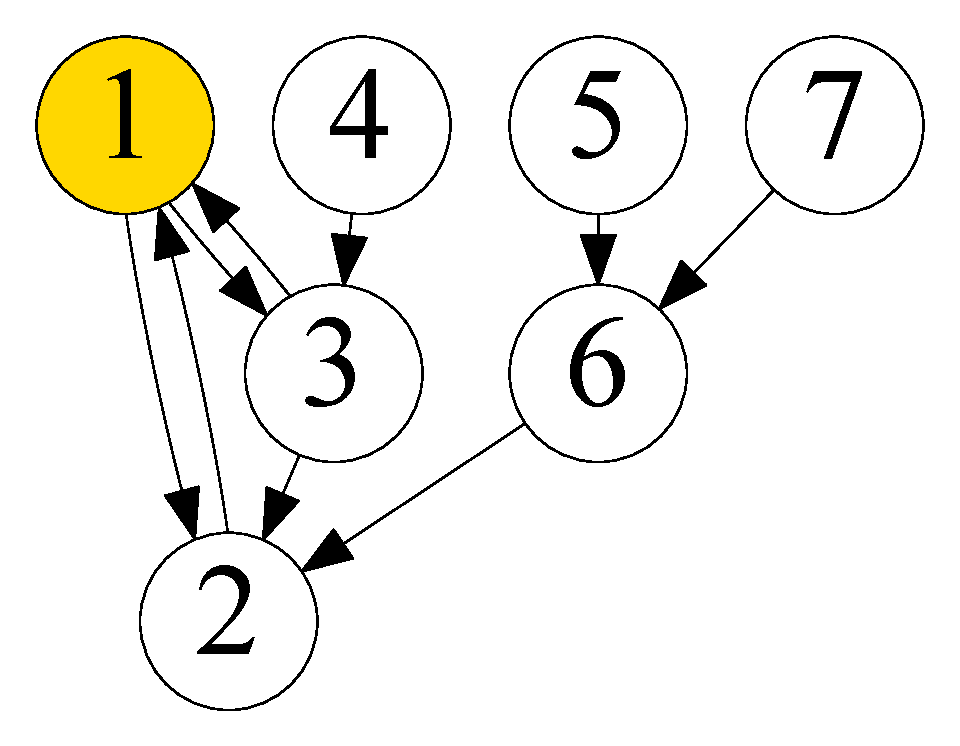
\includegraphics[width=0.3\columnwidth]{./alg_fig/fvs-eg}
\vspace{-1em}
\caption{An example of a directed graph; node 1 forms a feedback vertex set.}
\vspace{-1em}
\label{fig:fvs}
\end{figure}

% dependency graph
Our algorithms for IBVR are based on a graph representation of the transaction batches. Every batch $B$ of viable transactions induces a \emph{dependency graph} $G$; this is a directed graph whose nodes are the transactions in $B$ and whose edges are read-write dependencies.

\eat{
% first show if the graph is acyclic, then we are done
% if the graph is acyclic, we can construct prec
If $G$ is acyclic, then there exists a $\prec$ on $G$ that respects all read-write dependencies; we can construct it as follows. The edges in $G$ provide a strict partial order on $B$; for two nodes $t, t' \in G$, we order $t$ before $t'$ if and only if $t'$ is reachable from $t$ (they cannot both be reachable from each other by acyclicity). We complete the construction of $\prec$  by choosing any linear extension of this partial order.

% if there is a prec, we ensure no violation of read-write depedency exists
We need to show that if $t \prec t'$, then there is no read-write dependency from $t'$ to $t$. Suppose $t \prec t'$ and consider the nodes $t$ and $t'$ in $G$. Assume for a contradiction there is a read-write dependency from $t'$ to $t$. Then by construction, $G$ contains an edge from $t'$ to $t$, and by construction of $\prec$ we have $t' \prec t$; however, this contradicts the statements that $t \prec t'$ and that $\prec$ is strict.

Our family of algorithms for IBVR is based on constructing the dependency graph $G$ and finding a \emph{feedback vertex set} (FVS)~\cite{karp1972reducibility} on $G$. A FVS is a subset of vertices whose removal makes the graph acyclic. For example, consider the graph in Figure~\ref{fig:fvs}. The vertex 1 forms a FVS since the graph becomes acyclic after removing vertex 1 and its incoming and outgoing edges.

Finding a minimal-size $B'$ for IBVR is exactly the problem of finding the minimal (smallest-size) feedback vertex set on $G$. If we have a more complex objective function for IBVR, we can push the objective function into the FVS computation; we assign weights to the nodes to represent the desired transaction priorities, and look for a minimum-weight FVS. 

Once we find the FVS $B'$, removing the nodes in $B'$ from $G$ yields an acyclic graph that allows us to determine the desired serialization order $\prec$.
}

If $G$ is acyclic, then there exists a commit order $Q$ on $G$ that respects all read-write dependencies. We can construct $Q$ by repeatedly committing a transaction whose corresponding node in $G$ has no outgoing edge. This is always feasible when $G$ is acyclic.

Our family of algorithms for IBVR is based on constructing the dependency graph $G$ and finding a \emph{feedback vertex set} (FVS)~\cite{karp1972reducibility} on $G$. A FVS is a subset of vertices whose removal makes the graph acyclic. For example, consider the graph in Figure~\ref{fig:fvs}. The vertex 1 forms a FVS since the graph becomes acyclic after removing vertex 1 and its incoming and outgoing edges.

Finding a minimal-size $B'$ for IBVR is exactly the problem of finding the minimal (smallest-size) feedback vertex set on $G$. If we have a more complex objective function for IBVR, we can assign weights to the nodes to represent the desired transaction priorities, and look for a minimum-weight FVS. 

Once we find the FVS $B'$, removing the nodes in $B'$ from $G$ yields an acyclic graph that allows us to determine the desired commit order $Q$.

\eat{
\subsubsection{Complexity of FVS}\label{subsec:FVS_stateoftheart}

The directed graph FVS (DFVS) problem is well-studied as it has many applications, including deadlock detection, program verification, and Bayesian inference. 

It was listed among the first set of NP-complete problems~\cite{karp1972reducibility}. 
The state-of-the-art study~\cite{chen2008fixed} on the hardness of the problem has shown that it is \emph{fixed-parameter tractable}, that is, it can be solved in time $O(f(k)n^c)$ for a function $f(k)$ and a constant $c$ where the number $k$ and the function $f(k)$ are independent of the instance size $n$. \cite{chen2008fixed} proposes an exact algorithm for finding a minimal DFVS in $O(4^kk!n^{O(1)})$, where $n$ is the number of vertices and $k$ is the size of the minimal solution. 

DFVS is also APX-hard~\cite{kann1992approximability}. This means there exists a constant $c>1$ such that the existence of a polynomial-time approximate algorithm that achieves an approximation ratio strictly smaller than $c$ would imply $P=NP$. The best hardness result~\cite{dinur2005hardness} shows that it is NP-hard to approximate DFVS within a factor of 1.36, by an easy reduction from vertex cover. While it is still open whether there exists a constant factor approximation for DFVS, it is shown that it is NP-hard to approximate DFVS within any constant factor if the Unique Games Conjecture is true~\cite{guruswami2008beating}. The state-of-the-art algorithm has an approximation factor of $O(\log\tau\log\log\tau)$, where $\tau$ is the size of the exact solution, and a factor of $O(\log\tau^*\log\log\tau^*)$ for weighted directed graphs, where $\tau^*$ is the weight of the exact solution.

Despite the above hardness results, empirical studies have shown that simple greedy heuristics perform reasonably well when compared to more advanced algorithms~\cite{cutello2015targeting}. 
}


\subsection{Our IBVR Algorithms}
\label{subsec:validator_reordering:algorithm}

The directed graph FVS (DFVS) problem is well-studied as it has many applications, including deadlock detection, program verification, and Bayesian inference. It is NP-hard~\cite{karp1972reducibility} and APX-hard~\cite{kann1992approximability}, and it is still an open problem whether there exists any constant-factor approximation.

We need fast FVS algorithms to avoid increasing both transaction latencies and the number of aborts. We propose two greedy algorithms for finding feedback vertex sets -- one based on the graph's strongly connected components (SCCs) and the other based on sort. We also introduce a hybrid algorithm that makes strategic use of brute-force search, and consequently is slower but more precise.

All our IBVR algorithms begin by constructing the dependency graph $G$. We start with a set of transactions that have been batched at the validator and construct $B$ by discarding all non-viable transactions. We can identify such transactions by validating each transaction against all the updates prior to this batch.

Next, we create one node per transaction, and one edge per read-write dependency. To determine whether a read-write dependency holds from transaction $t'$ to $t$, we check whether $WS(t) \cap RS(t') \neq \emptyset$. If so, we add an edge from $t'$ to $t$. We can implement this by creating a hash table from the write sets and probing it with the read sets. The time complexity of building $G$ is $O(|B|+|R|+|W|)$, where $|B|$ is the size $B$, $|R|$ is the total number of reads, and $|W|$ is the total number of writes. 

We now process $G$ to find a feedback vertex set. Both before and during the execution of our FVS algorithms, we \emph{trim} the graph to remove all nodes which have no incoming edges and/or no outgoing edges; such nodes cannot participate in any cycles and are unnecessary to include in any FVS.


\begin{algorithm}[t]
\SetAlgoLined\DontPrintSemicolon
\SetKwProg{main}{Algorithm}{}{}
\main{GreedySccGraph($G$, $P$)}{
\KwIn{Directed graph $G$, policy $P$}
\KwOut{$V$, a feedback vertex set for $G$}
$V\gets \emptyset$\;
$G'\gets trim(G)$\;
$SCC = StronglyConnectedComponents(G')$\;
\For {$S \in SCC$} {
	$V\gets V\cup GreedyComponent(S, P)$\;
}
\Return{$V$}\;
}{}

\SetKwProg{sub}{Algorithm}{}{}
\sub{GreedyComponent($S$, $P$)}{
\KwIn{SCC $S$, policy $P$}
\KwOut{$V'$, a feedback vertex set for $S$}

\If {$S.size == 1$} {
	\Return{$\emptyset$}\;
}
$V' \gets \emptyset$\;
$v\gets select(S, P)$\;
$V'\gets V'\cup v$\;
$S'\gets delete(S, v)$\;
$V'\gets V'\cup GreedySccGraph(S', P)$\;
\Return{$V'$}\;
}{}

\caption{SCC-based greedy algorithm}
\label{alg:scc}
\end{algorithm}


\begin{algorithm}[t]
\SetAlgoLined\DontPrintSemicolon
\SetKwProg{main}{Algorithm}{}{}
\main{GreedySortGraph($G$, $P$, $k$)}{
\KwIn{Directed graph $G$, policy $P$, multi factor $k$}
\KwOut{$V$, a feedback vertex set for $G$}
$V\gets \emptyset$\;
$G\gets trim(G)$\;
\While {$G\neq \emptyset$} {
	\If {$G.size < k$} {
	 	$V\gets V\cup GreedySortGraph(G, P, 1)$\;
	 	break\;
	}
	$Q\gets sort(G, P)$\;
	\For {$i=1; i\leq k; ++i$} {
		$V\gets V\cup Q[i]$\;
		$G\gets remove(G, Q[i])$\;
	}
	$G\gets trim(G)$\;
}
\Return{$V$}\;
}{}
\caption{Sort-based greedy algorithm}
\label{alg:sort}
\end{algorithm}




\subsubsection{SCC-based greedy algorithm}

The intuition behind our first algorithm is that each cycle is contained in a strongly connected component of the graph, so we can process the components separately. After preprocessing, we partition the graph into SCCs. For a graph with $V$ vertices and $E$ edges, we can do this in time $O(|V|+|E|)$ using Tarjan's SCC algorithm~\cite{tarjan1972depth}.

Any SCCs that consist of a single node do not need to be considered further, as the one vertex involved cannot be on a cycle. If the SCC contains multiple vertices, we choose a vertex to remove according to some \emph{policy}. The policy is a ranking function on vertices and we choose the top-ranked vertex to remove. We now recurse on the remaining graph.

Algorithm~\ref{alg:scc} shows this in more detail. We begin by trimming and partitioning the graph into SCCs  (lines 3-4). We process each SCC $S$ using $GreedyComponent(S, P)$ (lines 5-7). This subroutine starts by eliminating SCCs of size one (lines 10-12). Next, it chooses a vertex $v$ from $S$, i.e. the top-ranked vertex under $P$ (line 14). It includes $v$ in the $FVS$ of $S$ (line 15), removes it from $S$ (line 16), and recursively calls $GreedySccGraph$ on the remaining graph (line 17). Finally, it returns the union of all the FVSs obtained in processing $S$ (line 18). When the top-level procedure $GreedyComponent(G, P)$ has processed all the SCCs of $G$, it returns the union of the FVSs obtained (line 8).

The policy $P$ is the heart of the algorithm and affects both its accuracy and running time. Fortunately, there is no trade-off between accuracy and running time; a more accurate policy will lead to a smaller FVS and faster termination. We discuss possible policies in Section \ref{subsec:validator_reordering:policy}.

\subsubsection{Sort-based greedy algorithm}

\begin{figure*}[t]
    \centering
    \begin{minipage}[b]{0.19\linewidth}
        \captionsetup{type=figure}
        \centering
        \subcaptionbox{original\label{fig:scc:g0}}
            {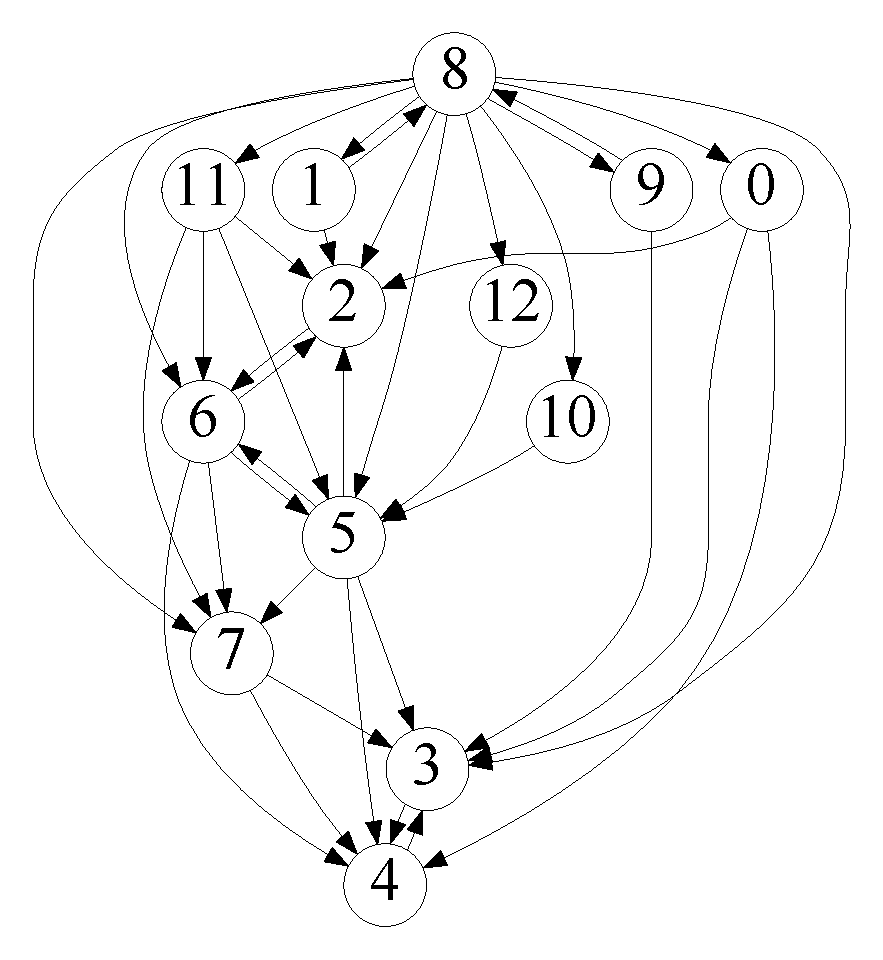
\includegraphics[width=\textwidth]{./alg_fig/scc-g0}}
   %     \vspace{-2em}
    \end{minipage}
   	\begin{minipage}[b]{0.19\linewidth}
        \centering
        \subcaptionbox{partition into SCCs\label{fig:scc:g1}}
                    {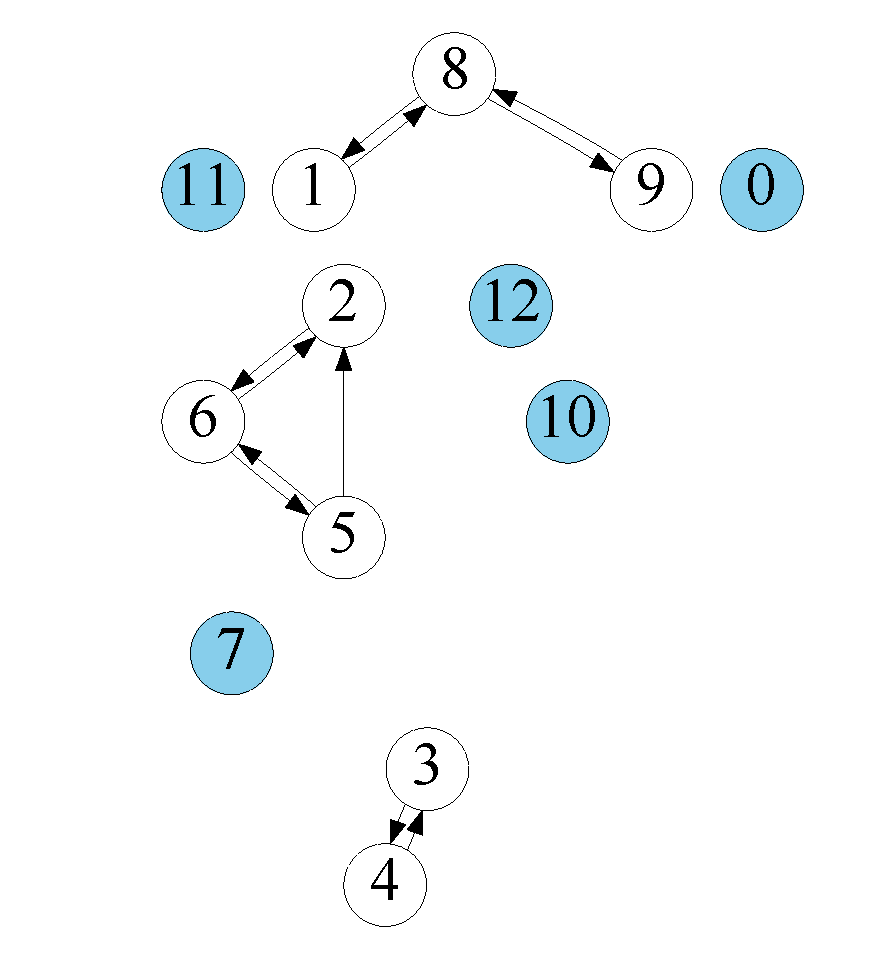
\includegraphics[width=\textwidth]{./alg_fig/scc-g1}}
    %    \vspace{-2em}
    \end{minipage}
    \begin{minipage}[b]{0.19\linewidth}
            \centering
            \subcaptionbox{add 3 to FVS\label{fig:scc:g3}}
                        {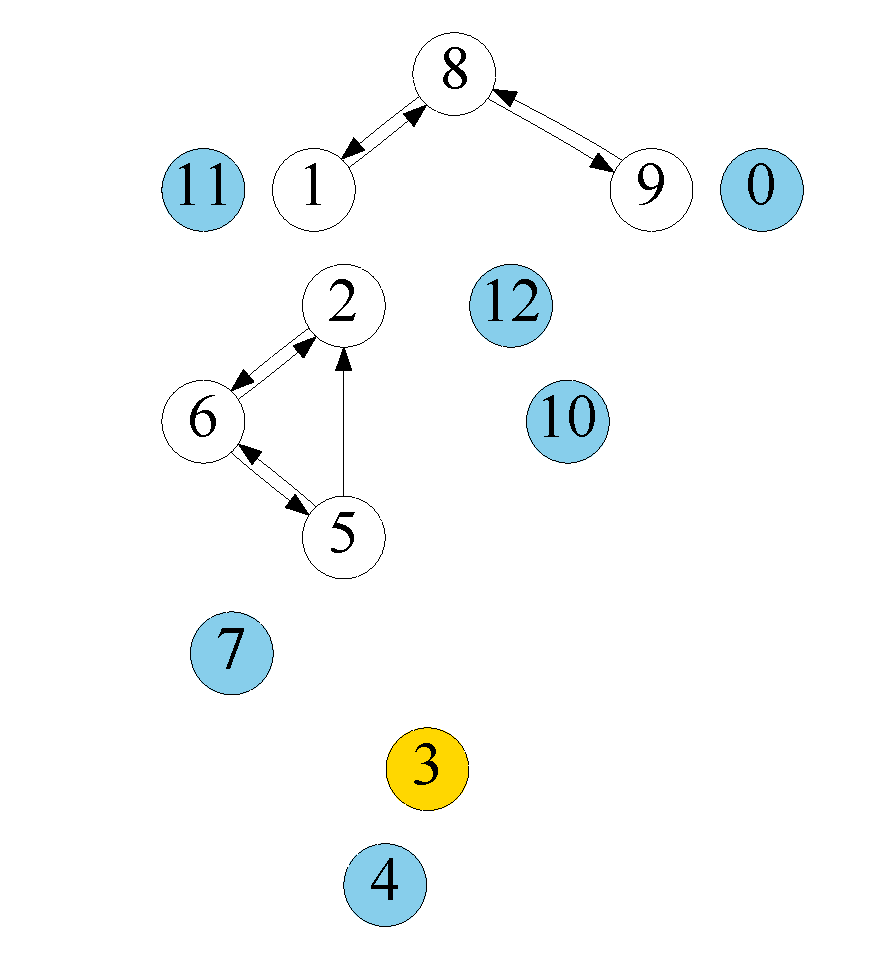
\includegraphics[width=\textwidth]{./alg_fig/scc-g3}}
     %       \vspace{-2em}
        \end{minipage}
    \begin{minipage}[b]{0.19\linewidth}
            \centering
            \subcaptionbox{add 6 to FVS\label{fig:scc:g5}}
                        {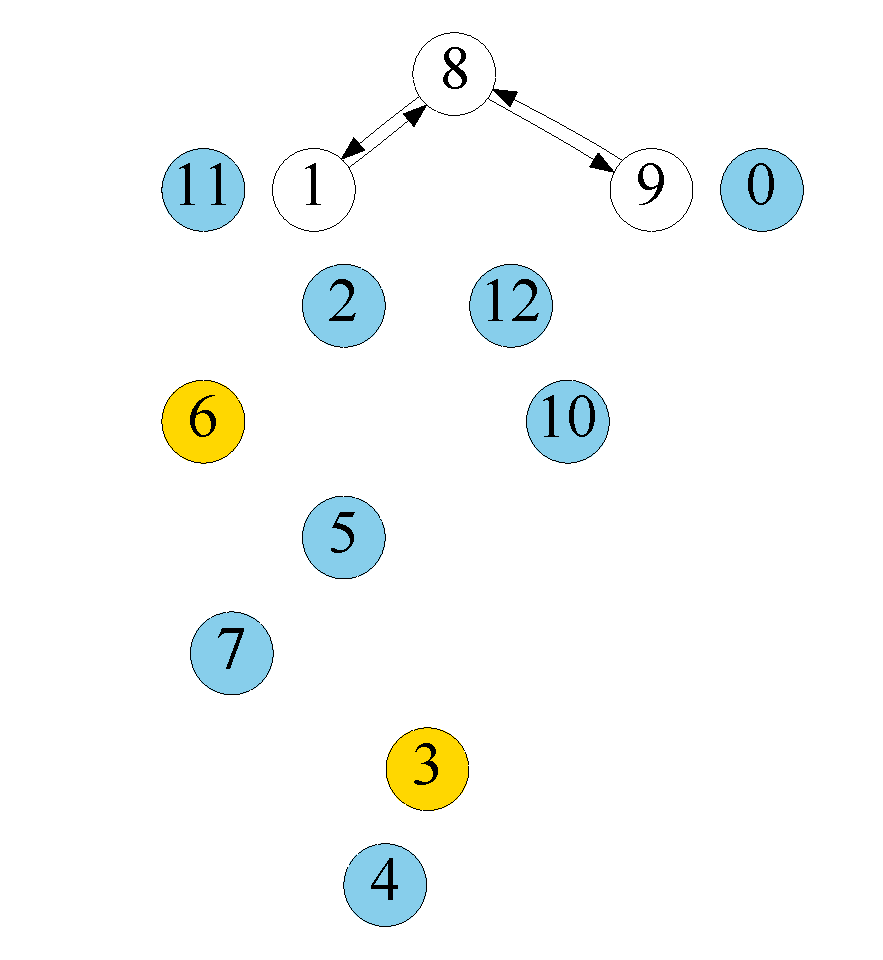
\includegraphics[width=\textwidth]{./alg_fig/scc-g5}}
      %      \vspace{-2em}
   		\end{minipage}                  
    \begin{minipage}[b]{0.19\linewidth}
            \centering
            \subcaptionbox{add 8 to FVS\label{fig:scc:g7}}
                        {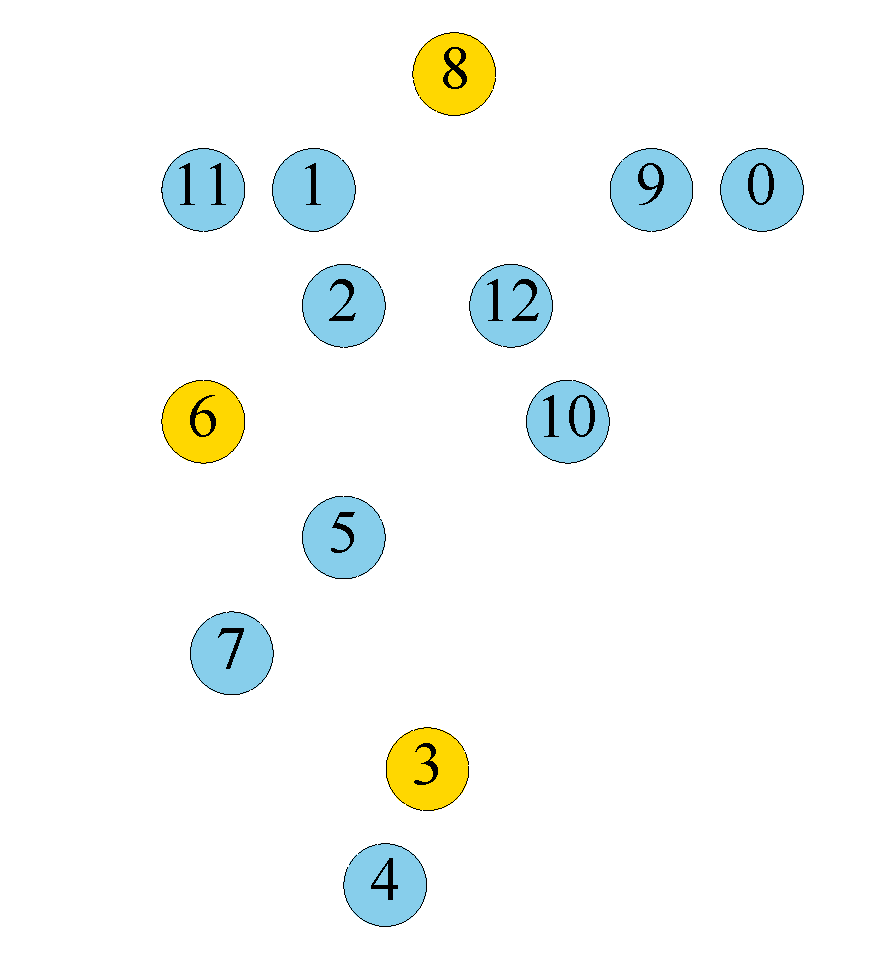
\includegraphics[width=\textwidth]{./alg_fig/scc-g7}}
       %     \vspace{-2em}
   		\end{minipage}  
  	\vspace{-1em}             
   \caption{An example of the SCC-based greedy algorithm using \texttt{prod-degree} policy}
   \vspace{-1em}
   \label{fig:scc}
\end{figure*}


\begin{figure*}[t]
    \centering
    \begin{minipage}[b]{0.19\linewidth}
        \captionsetup{type=figure}
        \centering
        \subcaptionbox{original\label{fig:simple:g0}}
        	{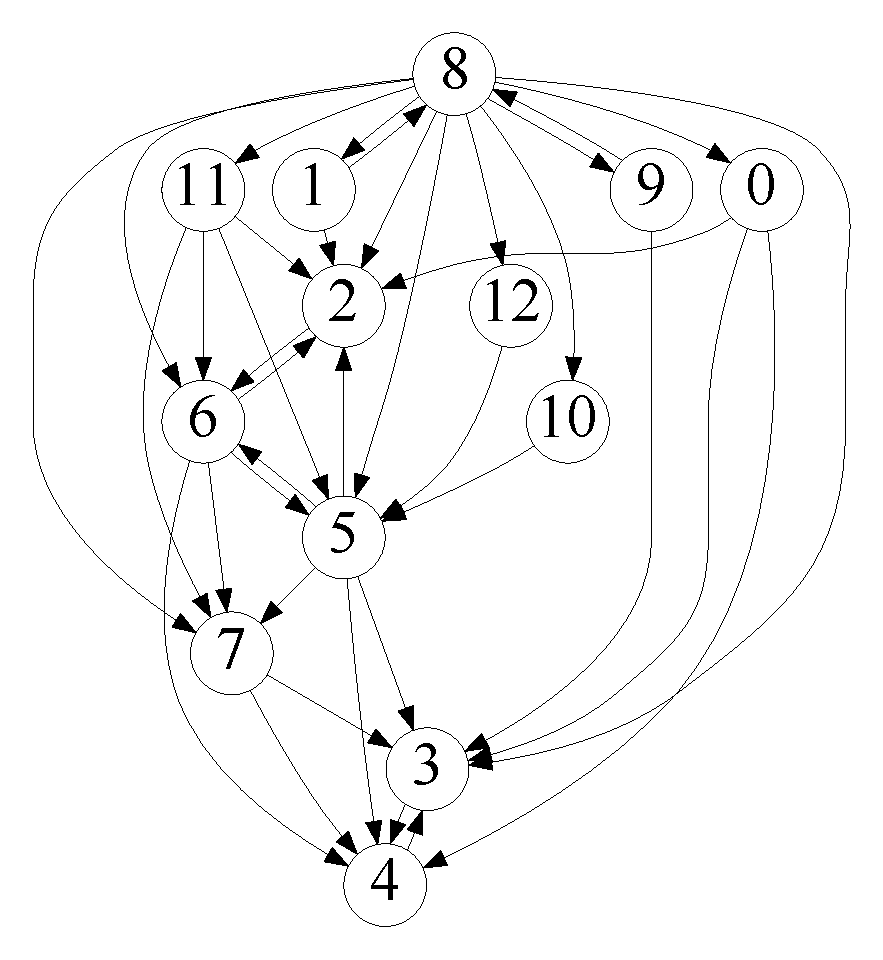
\includegraphics[width=\textwidth]{./alg_fig/simple-g0}}
   %     \vspace{-2em}
    \end{minipage}
    \begin{minipage}[b]{0.19\linewidth}
        \centering
        \subcaptionbox{add 5 to FVS\label{fig:simple:g2}}
        {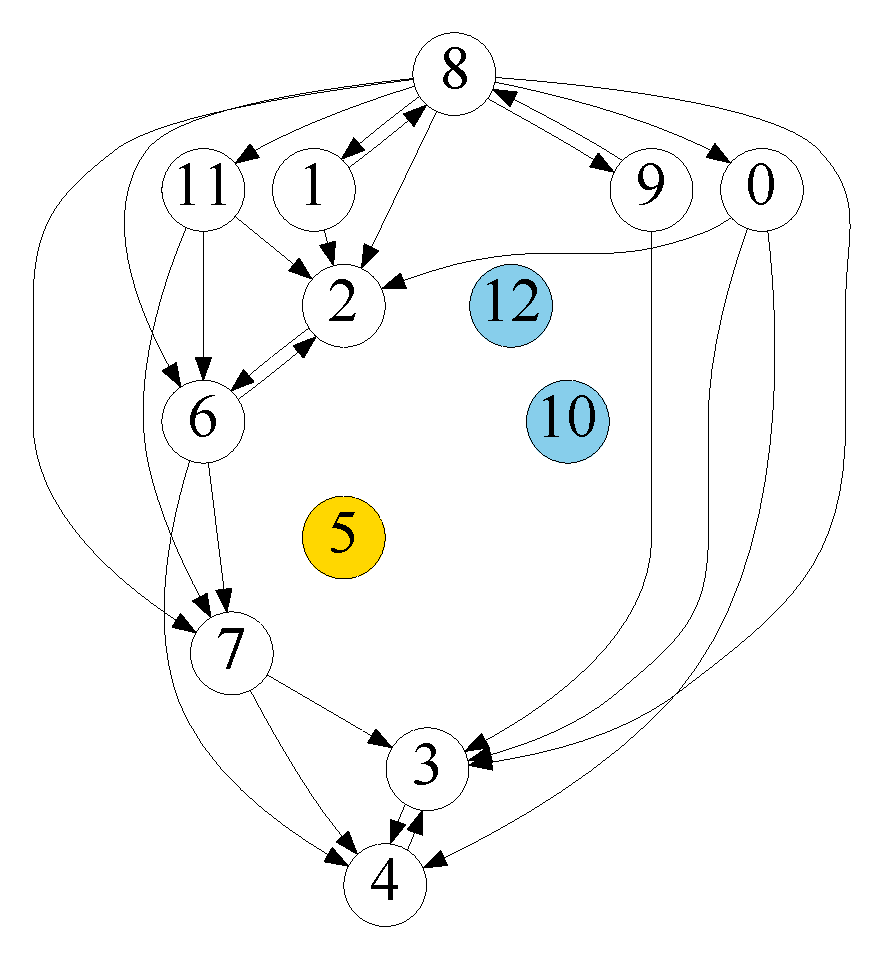
\includegraphics[width=\textwidth]{./alg_fig/simple-g2}}
    %    \vspace{-2em}
    \end{minipage}
    \begin{minipage}[b]{0.19\linewidth}
            \centering
        \subcaptionbox{add 8 to FVS\label{fig:simple:g4}}
            {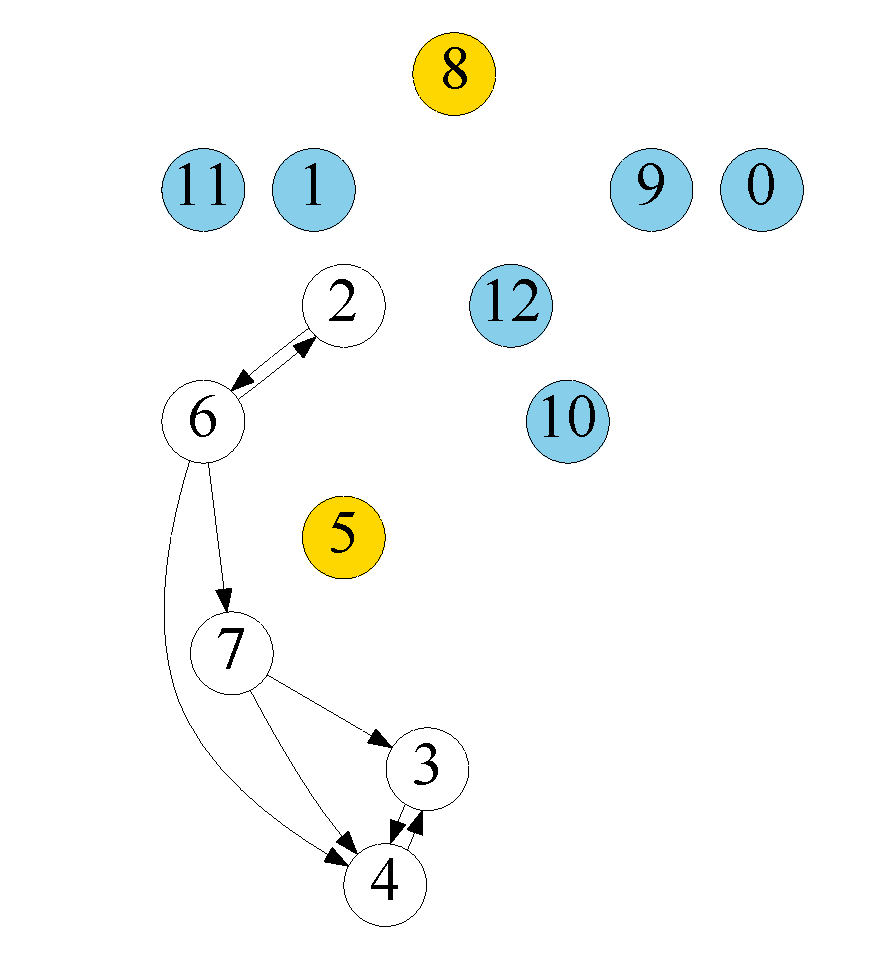
\includegraphics[width=\textwidth]{./alg_fig/simple-g4}}
     %       \vspace{-2em}
        \end{minipage}
    \begin{minipage}[b]{0.19\linewidth}
            \centering
             \subcaptionbox{add 6 to FVS\label{fig:simple:g6}}
			{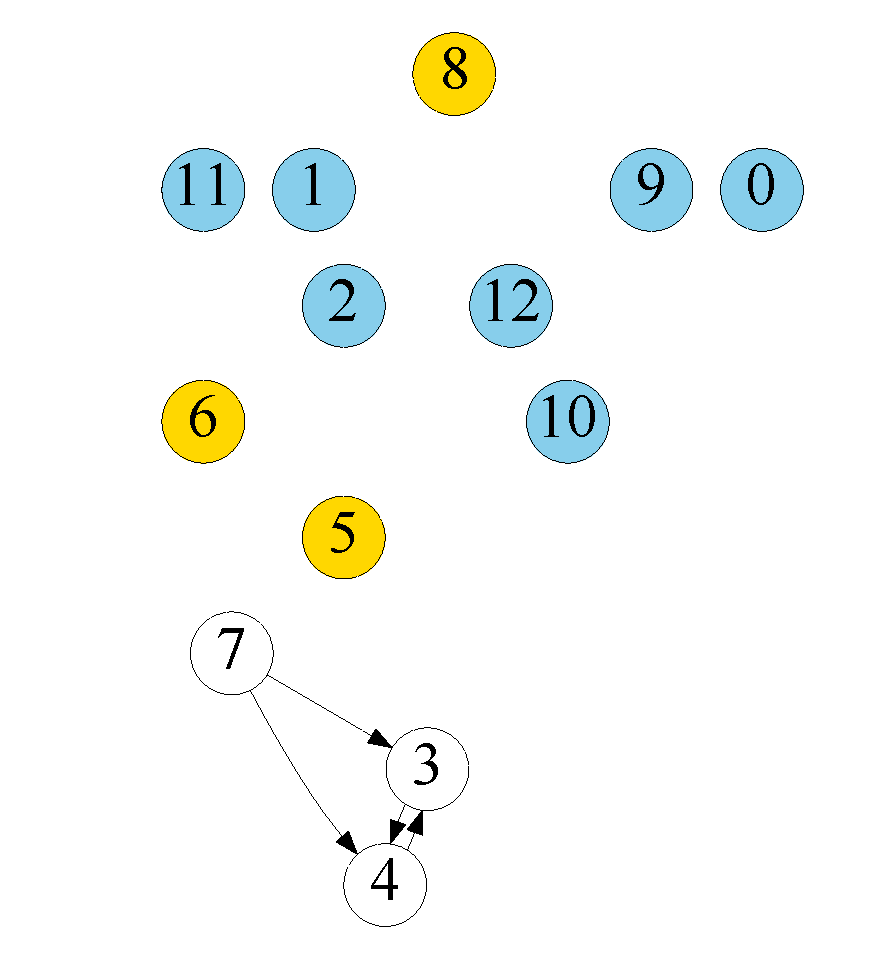
\includegraphics[width=\textwidth]{./alg_fig/simple-g6}}
      %      \vspace{-2em}
   		\end{minipage}                  
    \begin{minipage}[b]{0.19\linewidth}
            \centering
             \subcaptionbox{add 3 to FVS\label{fig:simple:g8}}
            {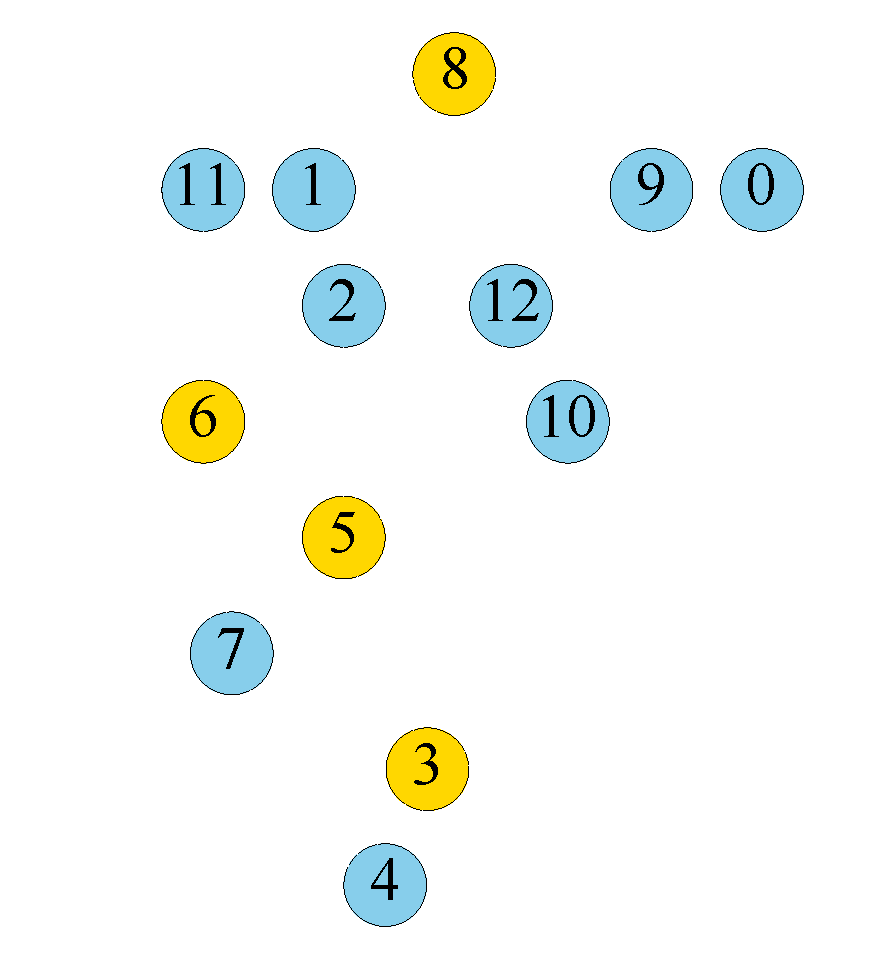
\includegraphics[width=\textwidth]{./alg_fig/simple-g8}}
       %     \vspace{-2em}
   		\end{minipage}
  	\vspace{-1em}             
   \caption{An example of the sort-based greedy algorithm using \texttt{prod-degree} policy and multi factor 1}
   \label{fig:simple}               
   \vspace{-1em}    	
\end{figure*}

Our first algorithm relies on a SCC partitioning routine that takes linear time in the size of the graph. As this routine is called several times during the course of the algorithm, it can cause a non-trivial overhead. Thus, we propose a second, faster greedy algorithm which uses sort-based heuristics to remove nodes.

Through empirical tests of the SCC-based greedy algorithm we found that nodes with certain properties are very likely to be included in a FVS. Such nodes generally have high in-degree and/or out-degree, for example. Our second algorithm is based on this observation; it sorts the nodes according to some ranking function (i.e., policy) $P$, and includes the top-ranked $k$ nodes in the FVS. We call $k$ the \emph{multi factor} of the algorithm. The algorithm removes these nodes and iterates on the remaining graph.

Algorithm~\ref{alg:sort} shows this in more detail. We trim the graph (line 3); if the graph has no more than $k$ nodes, we reduce the multi-factor to 1 (line 5-8). Otherwise, we sort the nodes into a queue $Q$ using $P$, and include the top-ranked $k$ nodes in $V$ (line 9-13).
After removing the selected nodes from $G$, we trim the remaining the graph again (line 14). We repeat until the graph is empty (line 4).

This algorithm is faster but less accurate than the SCC-based greedy algorithm. However,  our experiments in Section~\ref{sec:experiments} show that it produces comparably accurate results with the SCC-based algorithm in practice.

\subsubsection{Hybrid algorithm} We can combine the SCC-based greedy algorithm and the precise brute-force FVS search into a \emph{hybrid algorithm}. This is similar to the SCC-based greedy algorithm but runs a precise, brute-force FVS search in certain cases. Instead of processing all SCCs via the $GreedyComponent$ subroutine (lines 5-7 of Algorithm~\ref{alg:scc}), it runs the precise search when processing SCCs that are smaller than a certain \emph{threshold}, and the greedy subroutine $GreedyComponent$ on SCCs that are larger than the threshold. Adjusting the threshold allows us to trade off precision versus running time.


\subsection{Example}\label{subsec:alg_example}

Figures \ref{fig:scc} and \ref{fig:simple} show executions of the two greedy algorithms on the same graph. Both algorithms use a policy where the ranking of a node is the product of its in-degree and its out-degree, i.e. \texttt{prod-degree}.

Figure~\ref{fig:scc} shows the SCC-based greedy algorithm. The graph cannot be trimmed, so we partition it into SCCs. We remove all SCCs of size 1 -- namely nodes 0, 7, 10, 11, and 12 (Figure~\ref{fig:scc:g1}). There are three remaining SCCs. We first look at the component containing nodes 3 and 4. Since nodes 3 and 4 have the same product of in-degree and out-degree, we can add either one of them to the FVS. We choose node 3. Now node 4 has neither incoming nor outgoing edges, so it is trimmed (Figure~\ref{fig:scc:g3}). We repeat the process with the other components. For the SCC containing nodes 2, 5, and 6, we add node 6 to the FVS, as it has the largest product of in-degree and out-degree among the three nodes in this SCC. We now trim nodes 2 and 5 (Figure~\ref{fig:scc:g5}). Finally, we remove node 8 from the last component, and trim nodes 1 and 9 (Figure~\ref{fig:scc:g7}). This leaves us with a final FVS consisting of nodes 3, 6, and 8.

Figure~\ref{fig:simple} shows the same example using the sort-based greedy algorithm, with $k = 1$. After the first sort, we add node 5 to the FVS since it has the highest product of in-degree and out-degree. After eliminating node 5, nodes 10 and 12 have only incoming edges, and get trimmed (Figure~\ref{fig:simple:g2}). We sort the remaining nodes. This time, we add node 8 to the FVS, and trim nodes 0, 1, 9, 11 (Figure~\ref{fig:simple:g4}). We repeat this process with the remaining nodes until the graph is empty. This yields a FVS consisting of node 3, 5, 6, and 8 (Figure~\ref{fig:simple:g8}), which contains one more vertex than the FVS we obtained with the SCC-based algorithm.


\subsection{Algorithm Policies}
\label{subsec:validator_reordering:policy}

We now discuss policies for our greedy algorithms. As mentioned, a policy is a ranking function on vertices of the graph, and a good policy is one that ranks highly vertices which are likely to be in a desirable FVS. 

We first discuss the policies that aim at minimizing the number of conflicts, i.e. the size of the FVS. The simplest policy is \texttt{random} that assigns all nodes random rankings. Alternatively, we can rank nodes using degree-based heuristics, which use the intuition that the removal of a node will break many cycles if the node is high in some measurement of its graph degree. Such heuristics have  been shown to work well for FVS computation~\cite{cutello2015targeting}. For example, the policy \texttt{max-degree} chooses the node with the largest degree (either in-degree or out-degree), \texttt{sum-degree} chooses the node with the largest total degree (in-degree plus out-degree), and \texttt{prod-degree} chooses the node with the largest product of in-degree and out-degree. 

More sophisticated policies are possible if the system is optimizing for something beyond maximizing the number of commits. For example, we may want to bound the transactions' tail latency; we can do that by incorporating latency information in our policies. We can rank transactions based on how many times they have been aborted and restarted, breaking ties using degree-based heuristics; thus, transactions that have been restarted many times are less likely to enter the FVS and have a higher chance of committing. While this policy reduces the transaction tail latencies, it can increase the non-tail latencies, due to its suboptimality in finding the feedback vertex set. To alleviate this problem, we can devise policies that combine information about a transaction's number of restarts and its graph degree. For example, we can compute the ranking of a vertex as the product of its in-degree and out-degree divided by an exponential function of the number of restarts of the corresponding transaction. 

Finally, we can devise policies to handle \emph{hard transactions}. In many workloads some transactions are naturally more prone to conflicts, e.g., those that access many items and/or ``hot'' items. If we use graph degree based policies, such transactions are likely to be included in the FVS and aborted repeatedly. To avoid starvation, we can adjust our policies to increase the probability that these transactions can commit. For example, we can approximate the ``hardness'' of a transaction by the size of its read and write sets and include that as a weighting factor in the policy. 






\section{Batching and Reordering: Concepts}\label{sec:overview}

%In this section, we introduce our novel ideas of batching at the storage and the validator in an OCC system, and we formulate the resulting algorithmic problems. 

\emph{Batching} involves buffering a number of operations as they arrive at some component of the system and processing them as a group. 
Given a batch, we run a lightweight algorithm that analyzes the batch and then reorders the operations in the batch in order to reduce aborts. We will introduce two types of reordering opportunities: Storage batching and validator batching.

We first make a conceptual distinction between two types of transaction aborts: intra-batch and inter-batch aborts. Assume transaction $T$ abort due to its conflict with $T'$. If $T$ and $T'$ are in the same batch, we call the resulting abort of $T'$ an \emph{intra-batch abort}; otherwise, we call it an \emph{inter-batch abort}.
%Batching transactions that access the same objects together reduces inter-batch aborts. 
%There has been a lot of research on data clustering either online or offline~\cite{elmore2015squall, pavlo2012skew}, especially for fine-grained data partitioning. 
In this work, we focus on managing intra-batch aborts by strategically reordering the batched requests at storage and validator. 
Reducing inter-batch aborts is complementary to our effort. 

Our approach is agnostic to isolation levels as long as the reordering respects the corresponding definitions of conflicts for 
write-read, write-write, and read-write dependencies. In the remainder of this paper, we describe 
how to batch and reorder for serializability, but our techniques can be adapted accordingly to other isolation levels, 
such as snapshot isolation.

\eat{For example, in snapshot isolation, if the storage is multi-versioned and offers a consistent snapshot to reads, no reordering is needed. At the validator, two transactions in the same batch conflict with each other if they write to the same
object. Thus, we create a dependency graph based on write-write conflicts, and the other parts of the
protocol stay the same. For example, let $T_1$, $T_2$, and $T_3$ be in the same batch, where $T_1$ writes to
$X$, $T_2$ writes to $Y$, and $T_3$ writes to $X$ and $Y$. Committing $T_3$ will lead to the aborts of $T_1$ and $T_2$. But if
we choose to abort $T_3$, $T_1$ and $T_2$ can both commit. }

\subsection{Reordering at the Storage}\label{subsec:storage_reordering}
If a transaction reads a stale version of an object from the storage layer, it is bound to 
abort at the validator as it conflicts with the update from a committed transaction. 
Thus, applying updates at the storage layer as early as possible can 
reduce the chance of aborts for incoming transactions.

We implement this idea as follows. We buffer a number of read and write requests from transactions into batches. 
As a batch of requests arrives at the storage layer, for each object, we apply the highest-version write request on that object. It is safe to discard all other writes on that object as explained in Section~\ref{sec:background}.\footnote{Recall that we assume full serializability; this may be different for snapshot isolation.} 
Next, we handle all the read requests for the same object. This strategy works very well for reducing intra-batch aborts, 
as it ensures that all available writes by committed transactions are applied to all objects before we handle any read requests on these objects. 

\subsection{Reordering at the Validator}\label{subsec:validator_reordering}

In validator batching, we buffer transaction validation requests at the validator as they arrive. Once a batch has been collected, the validator can reduce intra-batch aborts by selectively aborting transactions while choosing a good validation (and thus resulting serialization) order.
Such intra-batch transaction reordering can be done with several goals in mind. We can simply minimize intra-batch transaction aborts, i.e., we maximize the number of transactions in each batch that commit. Alternatively, we may also want to prioritize certain transactions to have a greater chance of committing. For example, if we want to reduce the transactions' tail latency, we can increase a transaction's priority every time it has to abort and restart. Priorities could also be related to external factors, e.g., a transaction's monetary value or an external, application-defined transaction priority. 
%These choices suggest a range of possible policies; we explore them in the next section.

%\subsection{Intra-Batch Validator Reordering (IBVR)}\label{sec:ibvr}
%\label{subsec:validator_reordering:algorithm}
We define the problem of intra-batch validator reordering (IBVR) more formally. A \emph{batch} $B$ is a set of transactions to be validated. We assume all transactions $t \in B$ are \emph{viable}, that is, no $t \in B$ conflicts with a previously committed transaction. If there are non-viable transactions in $B$, they can be removed in preprocessing, as they must always abort.
Given $B$, the goal of IBVR is to find a subset $B' \subseteq B$ of transactions to abort such that there is a serialization order $\prec$ for the 
the remaining transactions $B \setminus B'$, and all of the transactions in $B \setminus B'$ commit when validated in this order.
%that must abort due to intra-batch aborts. IBVR must also find a 
%strict (i.e. asymmetric) 
%total order $\prec$ on $B \setminus B'$ that \emph{respects all read-write dependencies}; that is, for $t,t'\in B \setminus B'$, if $t \prec t'$, then there is no read-write dependency from $t'$ to $t$.
We then processes each batch by running IBVR to identify $B'$ and $\prec$, aborting all the transactions in $B'$,  and validating the transaction in $B \setminus B'$  
in the order $\prec$. 
%By the constraint we gave on $\prec$ above, and from the discussion in Section~\ref{sec:background}, $\prec$ is guaranteed to be a valid serialization order that allows all transactions in $B \setminus B'$  to commit.
%Note that there is always a trivial solution to any IBVR instance: we can choose $B'$ to be all the elements of $B$ except one, so that $B \setminus B'$ has cardinality one. Such solutions are not useful; therefore, every instance of IBVR is associated with an \emph{objective function} on $B'$, and the goal is to find a $B'$ that maximizes the objective function. An example objective function could be the size of $B'$ (smaller is better), or a more complex function that takes into account transaction weights (e.g. priorities).
%Given $B$, the goal of IBVR is to find a $B' \subseteq B$ of transactions that must abort due to intra-batch aborts, and a commit order $Q$ for the remaining transactions that respects all read-write dependencies. The validator processes each batch by running IBVR to identify $B'$ and $Q$, aborting all the transactions in $B'$ and committing remaining transactions in the order of $Q$.
Note that there is always a trivial solution to any IBVR instance, namely to abort all transactions but one. 
This solution is not useful; therefore, every instance of
IBVR is associated with an \emph{objective function} on $B'$, and the goal is to
find a $B'$ that maximizes the objective function. A simple objective function
is the size of $B'$ (the fewer transactions to abort the better), and more complex functions can take transaction priorities
or the tail latency of transactions into
account. We call this objective function a \emph{policy} $P$.

\begin{figure}[t]
	\centering
	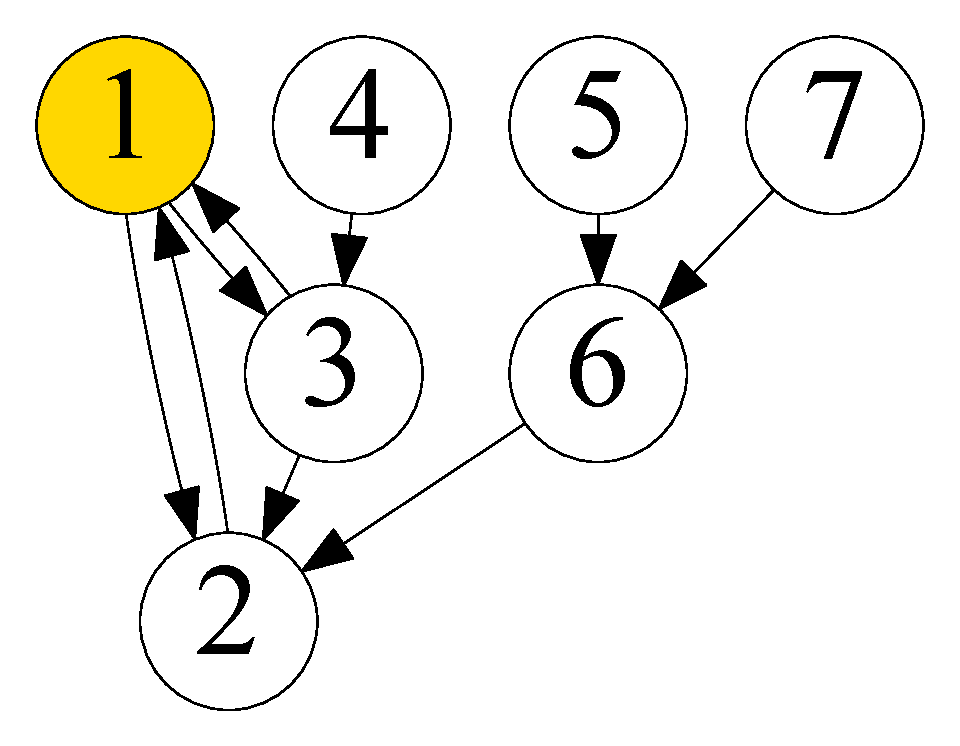
\includegraphics[width=0.3\columnwidth]{./alg_fig/fvs-eg}
	%\vspace{-1em}
	\caption{An example of a directed graph; node 1 forms a feedback vertex set.}
	%\vspace{-1em}
	\label{fig:fvs}
\end{figure}

% dependency graph
%Our algorithms for IBVR are based on a graph representation of the transaction batches. 
How do we compute $B'$? We observe that every batch $B$ of viable transactions 
has an associated \emph{dependency graph} $G$, a directed graph whose nodes are the transactions in $B$ and whose edges are read-write dependencies.
If $G$ is acyclic, then there exists a commit order $Q$ on $G$ that respects all read-write dependencies. We can construct $Q$ by repeatedly committing a transaction whose corresponding node in $G$ has no outgoing edge using a topological sort. 

If $G$ is not acyclic, we can model this problem as an instance of the feedback vertex set problem. 
%show that the of finding a minimal $B'$ is NP-hard by reducing the NP-hard directed feedback vertex set problem 
%to the selection of a minimal $B'$~\cite{karp1972reducibility}. 
A feedback vertex set (FVS) of a directed graph is a subset of vertices whose removal makes the graph acyclic. For example, consider the graph in Figure~\ref{fig:fvs}. Vertex 1 forms a FVS since the graph becomes acyclic after removing Vertex 1 and its incoming and outgoing edges. Finding a minimal-size $B'$ for IBVR is exactly the problem of finding the minimal (smallest-size) feedback vertex set on $G$. If we have a more complex objective function for IBVR, we can assign weights to the nodes to represent the desired transaction priorities, and look for a minimum-weight FVS. 
Once we find the FVS $B'$, removing the nodes in $B'$ from $G$ yields an acyclic graph that determines the desired commit order $Q$.
The directed graph FVS (DFVS) problem is well-studied as it has many applications, including deadlock detection, program verification, and Bayesian inference. Unfortunately, it is NP-hard and APX-hard~\cite{kann1992approximability, karp1972reducibility}, and it is still an open problem whether there exists any constant-factor approximation.
We propose several practical algorithms for finding a FVS in the next section.


%%%%%%%%%%%%%%%%%%%%%%%%%%%%%%%%%%%%%%%%%%%%%%%%%%%%%%%%%%%%%%%%%%%%%%
%%%%%%%%%%%  VALIDATOR BATCHING: OUR ALGORITHMS
%%%%%%%%%%%%%%%%%%%%%%%%%%%%%%%%%%%%%%%%%%%%%%%%%%%%%%%%%%%%%%%%%%%%%%

\section{Validator Batching}
\label{sec:valbatching}
All our IBVR algorithms begin by constructing the dependency graph $G$. 
%We start with a batch of transactions and construct $B$ by discarding all non-viable transactions. We can identify such transactions by validating each transaction against all the updates prior to this batch.
We create one node per transaction, and one edge per read-write dependency. 
To determine whether a read-write dependency holds from transaction $t'$ to $t$, we check whether $WS(t) \cap RS(t') \neq \emptyset$. If so, we add an edge from $t'$ to $t$. We implement this by creating a hash table from the write sets and probing it with the read sets. Since a read in $t$ can potentially conflict with all the other transactions in the batch, the time complexity to probe the hash table for a single read is $O(|B|)$, where $|B|$ is the size of the batch. The complexity of building $G$ is thus $O(|B|^2+|R|+|W|)$, where $|R|$ is the total number of reads, and $|W|$ is the total number of writes. 

We now process $G$ to find a feedback vertex set. Both before and during the
execution of our FVS algorithms, we \emph{trim} the graph to remove all the nodes
that have no incoming edges and/or no outgoing edges since such nodes cannot
participate in any cycles.

\subsection{Algorithms}
\label{subsec:validator_reordering:algorithm}

\begin{algorithm}[t]
	\SetAlgoLined\DontPrintSemicolon
	\SetKwProg{main}{Algorithm}{}{}
	\main{GreedySccGraph($G$, $P$)}{
		\KwIn{Directed graph $G$, policy $P$}
		\KwOut{$V$, a feedback vertex set for $G$}
		$V\gets \emptyset$\;
		$G'\gets trim(G)$\;
		$SCC = StronglyConnectedComponents(G')$\;
		\For {$S \in SCC$} {
			$V\gets V\cup GreedyComponent(S, P)$\;
		}
		\Return{$V$}\;
	}{}
	
	\SetKwProg{sub}{Algorithm}{}{}
	\sub{GreedyComponent($S$, $P$)}{
		\KwIn{SCC $S$, policy $P$}
		\KwOut{$V'$, a feedback vertex set for $S$}
		
		\If {$S.size == 1$} {
			\Return{$\emptyset$}\;
		}
		$v\gets SelectVertexByPolicy(S, P)$\;
		$S'\gets GetGraphAfterVertexRemoval(S, v)$\;
		\Return{$v \cup GreedySccGraph(S', P)$}\;
	}{}
	
	\caption{SCC-based greedy algorithm}
	\label{alg:scc}
\end{algorithm}


\begin{algorithm}[t]
	\SetAlgoLined\DontPrintSemicolon
	\SetKwProg{main}{Algorithm}{}{}
	\main{GreedySortGraph($G$, $P$, $k$)}{
		\KwIn{Directed graph $G$, policy $P$, multi factor $k$}
		\KwOut{$V$, a feedback vertex set for $G$}
		$V\gets \emptyset$\;
		$G\gets trim(G)$\;
		\While {$G\neq \emptyset$} {
			\If {$G.size < k$} {
				$V\gets V\cup GreedySortGraph(G, P, 1)$\;
				break\;
			}
			$Q\gets QuickSelectVertexByPolicy(G, P, k)$\;
			\For {$i=1; i\leq k; ++i$} {
				$V\gets V\cup Q[i]$\;
				$G\gets GetGraphAfterVertexRemoval(G, Q[i])$\;
			}
			$G\gets trim(G)$\;
		}
		\Return{$V$}\;
	}{}
	\caption{Sort-based greedy algorithm}
	\label{alg:sort}
\end{algorithm}

{\bf SCC-Based Greedy Algorithm.} The intuition behind our first algorithm is that each cycle must be contained in a strongly connected component of the graph. After preprocessing, we partition the graph into SCCs. For a graph with $V$ vertices and $E$ edges, we can do this in time $O(|V|+|E|)$ using Tarjan's SCC algorithm~\cite{tarjan1972depth}.

Nodes in SCCs of size one cannot belong to any cycle. For a SCC that contains
more than one node, we choose a vertex to remove according to a \emph{policy}. The policy is a ranking function over vertices, and we greedily choose the top-ranked vertex to remove. We then recurse on the remaining graph. Algorithm~\ref{alg:scc} shows the details of this procedure. We begin by trimming and partitioning the graph into SCCs  (lines 3-4). We process each SCC $S$ using $GreedyComponent(S, P)$ (lines 5-7). This subroutine starts by eliminating SCCs of size one (lines 10-12). Next, it chooses the top-ranked vertex $v$ from $S$ under Policy $P$ (line 13). It removes $v$ from $S$ and recursively calls $GreedySccGraph$ on the remaining graph $S'$ (line 14 - 15). Finally, it returns the union of all the FVSs obtained in processing $S$ (line 15). When the top-level procedure $GreedySccGraph(G, P)$ has processed all the SCCs of $G$, it returns the union of the FVSs obtained (line 8).
% Time complexity analysis
Trimming and updating the graph after removing a node take $O(|V| + |E|)$ per
graph in total, since each node / edge can be removed only once. In the worst case, e.g., in a fully connected graph, we may only remove one node per iteration. Since SCC takes $O(|V|+|E|)$ per iteration, the time complexity of this algorithm is $O(|V|(|V|+|E|))$.
The policy $P$ is at the heart of the algorithm, and it ranks vertices which are likely to be included in a desirable FVS highly. We discuss possible policies in Section \ref{subsec:validator_reordering:policy}.

\begin{figure*}[t]
	\centering
	\begin{minipage}[b]{0.19\linewidth}
		\captionsetup{type=figure}
		\centering
		\subcaptionbox{original\label{fig:scc:g0}}
		{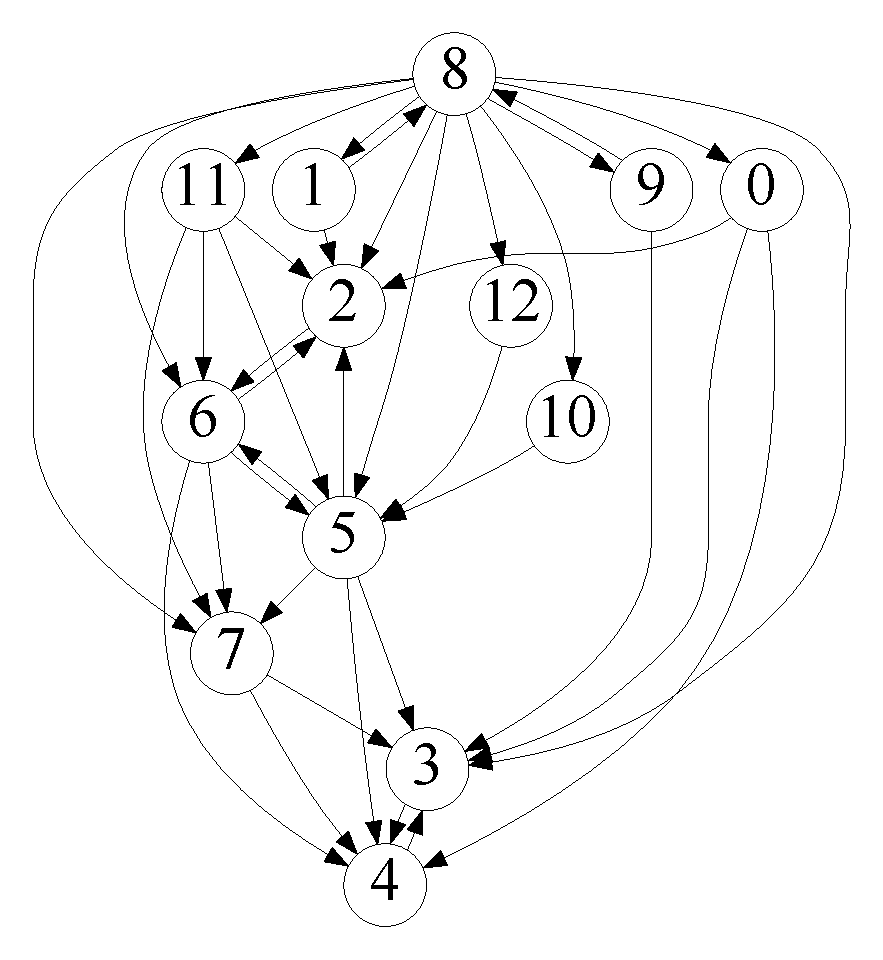
\includegraphics[width=\textwidth]{./alg_fig/scc-g0}}
		%     \vspace{-2em}
	\end{minipage}
	\begin{minipage}[b]{0.19\linewidth}
		\centering
		\subcaptionbox{partition into SCCs\label{fig:scc:g1}}
		{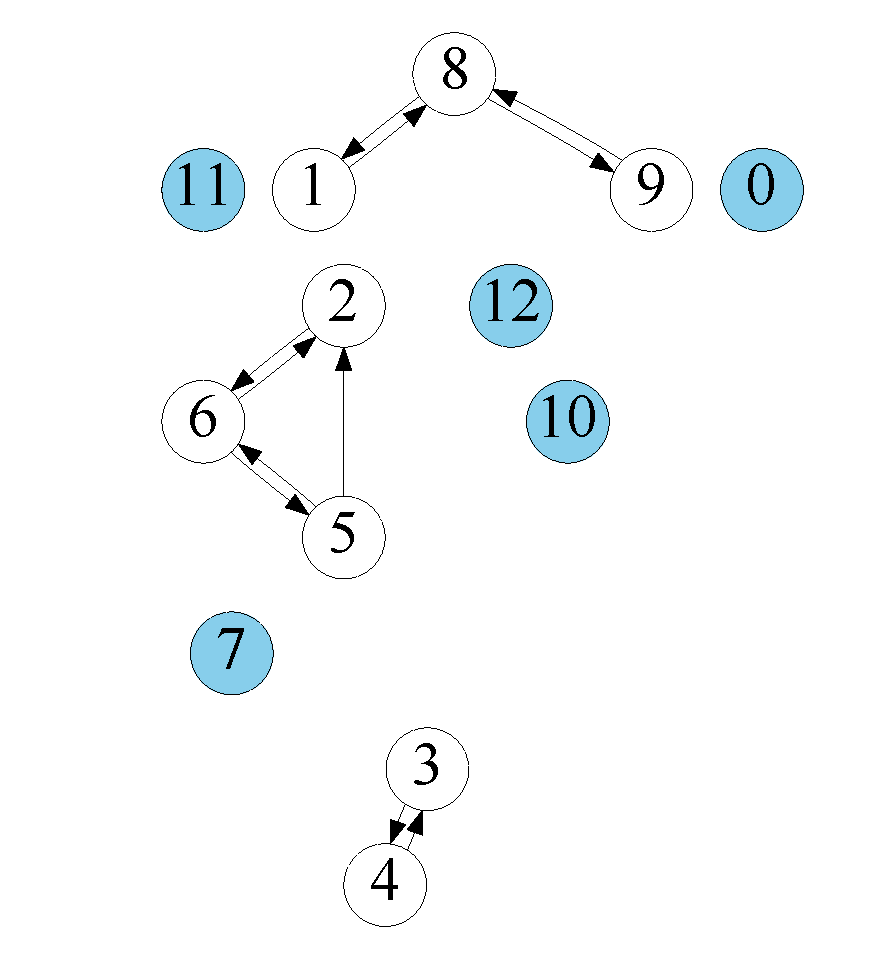
\includegraphics[width=\textwidth]{./alg_fig/scc-g1}}
		%    \vspace{-2em}
	\end{minipage}
	\begin{minipage}[b]{0.19\linewidth}
		\centering
		\subcaptionbox{add 3 to FVS\label{fig:scc:g3}}
		{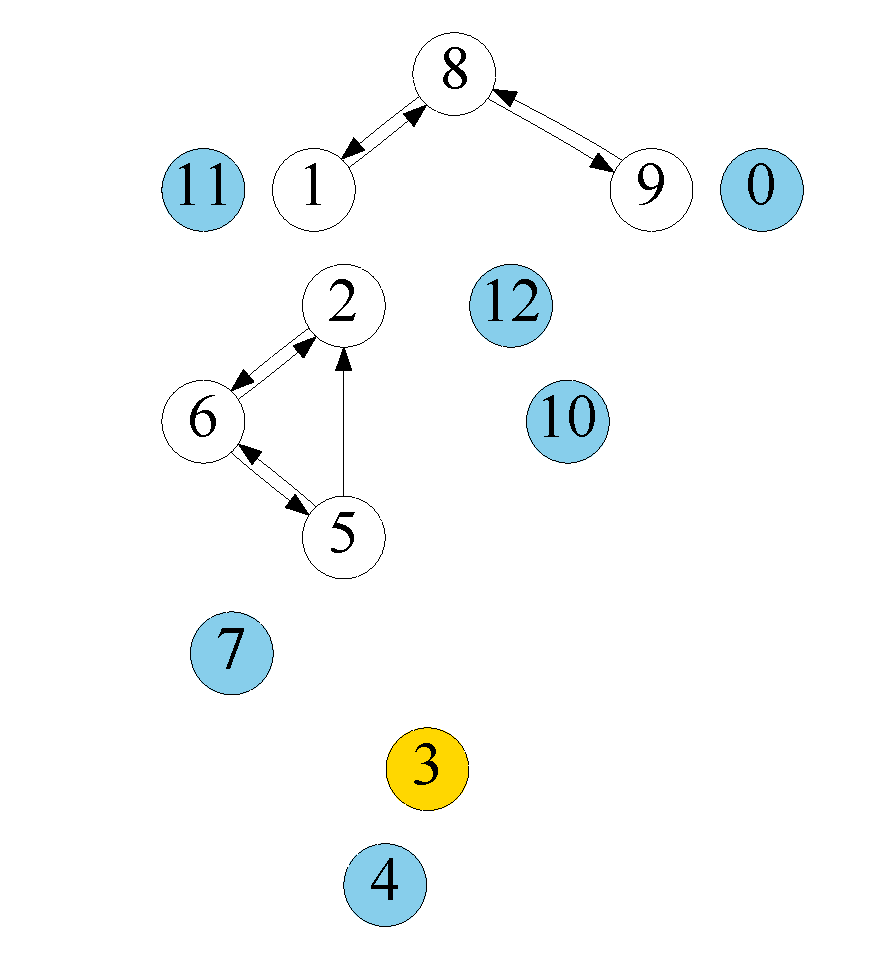
\includegraphics[width=\textwidth]{./alg_fig/scc-g3}}
		%       \vspace{-2em}
	\end{minipage}
	\begin{minipage}[b]{0.19\linewidth}
		\centering
		\subcaptionbox{add 6 to FVS\label{fig:scc:g5}}
		{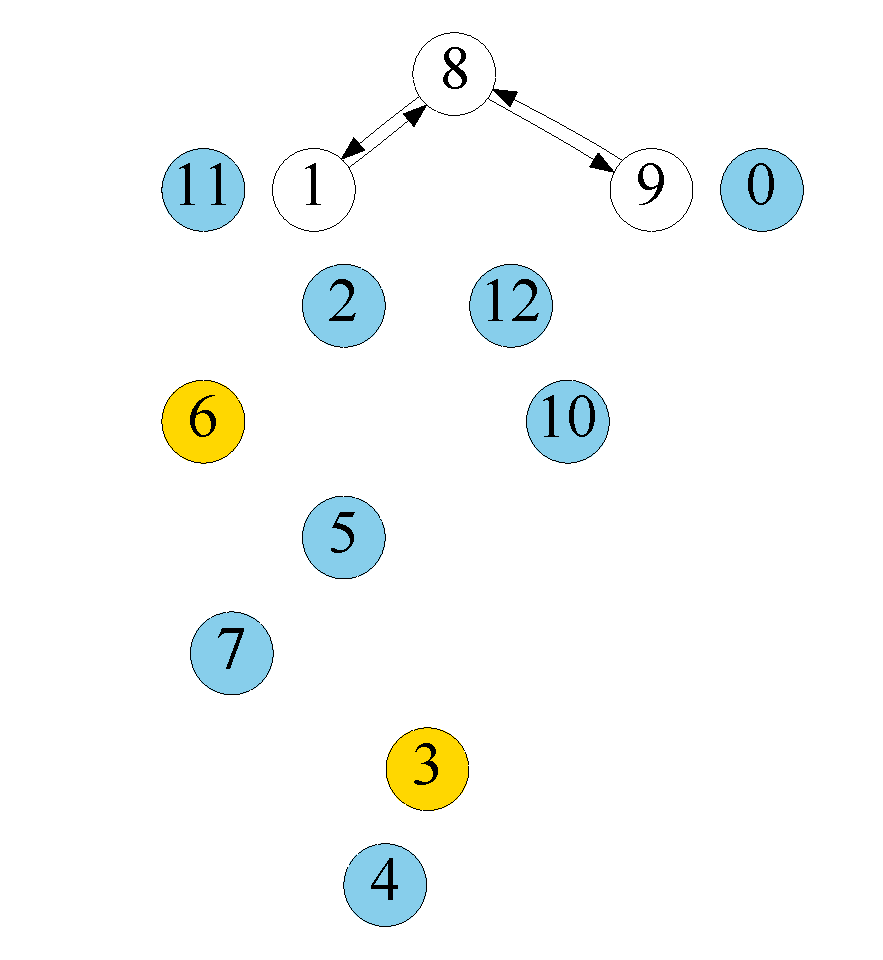
\includegraphics[width=\textwidth]{./alg_fig/scc-g5}}
		%      \vspace{-2em}
	\end{minipage}                  
	\begin{minipage}[b]{0.19\linewidth}
		\centering
		\subcaptionbox{add 8 to FVS\label{fig:scc:g7}}
		{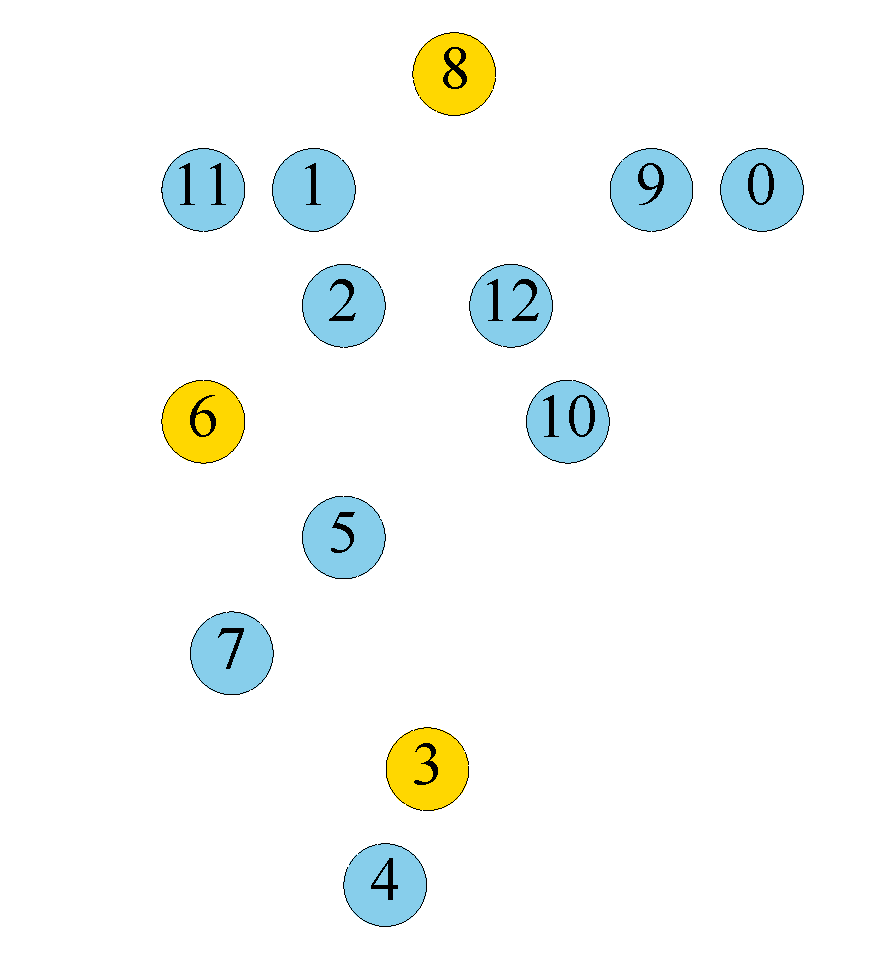
\includegraphics[width=\textwidth]{./alg_fig/scc-g7}}
		%     \vspace{-2em}
	\end{minipage}  
	%\vspace{-1em}             
	\caption{An example of the SCC-based greedy algorithm using \texttt{prod-degree} policy. Blue nodes are trimmed during the algorithm, and yellow nodes form the FVS.}
	%\vspace{-1em}
	\label{fig:scc}
\end{figure*}

{\bf An example.} Figure~\ref{fig:scc} shows an instance of the SCC-based greedy algorithm that aims at minimizing the size of FVS, with a policy $P$ selecting the node with the largest product of its in-degree and out-degree, i.e., \texttt{prod-degree}. The graph cannot be trimmed, so we partition it into SCCs. We remove all SCCs of size 1 --  Nodes 0, 7, 10, 11, and 12 (Figure~\ref{fig:scc:g1}). There are three remaining SCCs. We first look at the component containing Nodes 3 and 4. Since Nodes 3 and 4 have the same product of in-degree and out-degree, we can add either one of them to the FVS. We choose Node 3. Now Node 4 has neither incoming nor outgoing edges, so it is trimmed (Figure~\ref{fig:scc:g3}). We repeat the process with the other components. For the SCC containing Nodes 2, 5, and 6, we add Node 6 to the FVS, as it has the largest product of in-degree and out-degree among the three nodes in this SCC. We now trim Nodes 2 and 5 (Figure~\ref{fig:scc:g5}). Finally, we remove Node 8 from the last component, and trim Nodes 1 and 9 (Figure~\ref{fig:scc:g7}). This leaves us with a final FVS consisting of Nodes 3, 6, and 8.

{\bf Sort-Based Greedy Algorithm.} Our first algorithm relies on a SCC partitioning routine that takes linear time in the size of the graph. As this routine is called several times throughout the algorithm, it can cause a non-trivial overhead. Here we propose a faster greedy algorithm using a sort-based approach to remove nodes. Through extensive empirical tests of the SCC-based greedy algorithm, we found that at each iteration, all the top ranked nodes in the graph are very likely to be included in the final FVS. Our second algorithm is based on this observation; it sorts the nodes according to a policy $P$, and includes the $k$ top-ranked nodes in the FVS. We call $k$ the \emph{multi factor} of the algorithm. The algorithm removes these nodes and iterates on the remaining graph.

Algorithm~\ref{alg:sort} shows this in more detail. We start by trimming the graph (line 3); if the graph has no more than $k$ nodes, we reduce the multi-factor to 1 (line 5-8). Otherwise, we sort and select top ranked $k$ nodes into a queue $Q$ using $P$ with the Quickselect algorithm~\cite{hoare61cacm}, and include the $k$ nodes in $V$ (line 9-13).
After removing the selected nodes from $G$, we trim the remaining the graph
again (line 14). We repeat this procedure until the graph is empty (line 4). 
% time complexity analysis.
As with the previous algorithm, updating the graph after removing a node and \emph{trim} takes $O(|V|+|E|)$ in total. Updating the weights of the remaining nodes takes $O(|V|)$ per iteration. The
Quickselect algorithm~\cite{hoare61cacm} has an amortized time complexity of
$O(|V|)$. In the worst case, it will take $O(|V|/k)$ iterations to terminate. So
the overall time complexity is $O(|V|^2/k + |V| + |E|)$.
This algorithm has smaller time complexity than the SCC-based greedy algorithm, and we can increase $k$ to further trade accuracy for shorter runtime. As we will see in Section~\ref{sec:experiments}, it produces results of comparable accuracy to the SCC-based algorithm in practice.

\begin{figure*}[t]
	\centering
	\begin{minipage}[b]{0.19\linewidth}
		\captionsetup{type=figure}
		\centering
		\subcaptionbox{original\label{fig:simple:g0}}
		{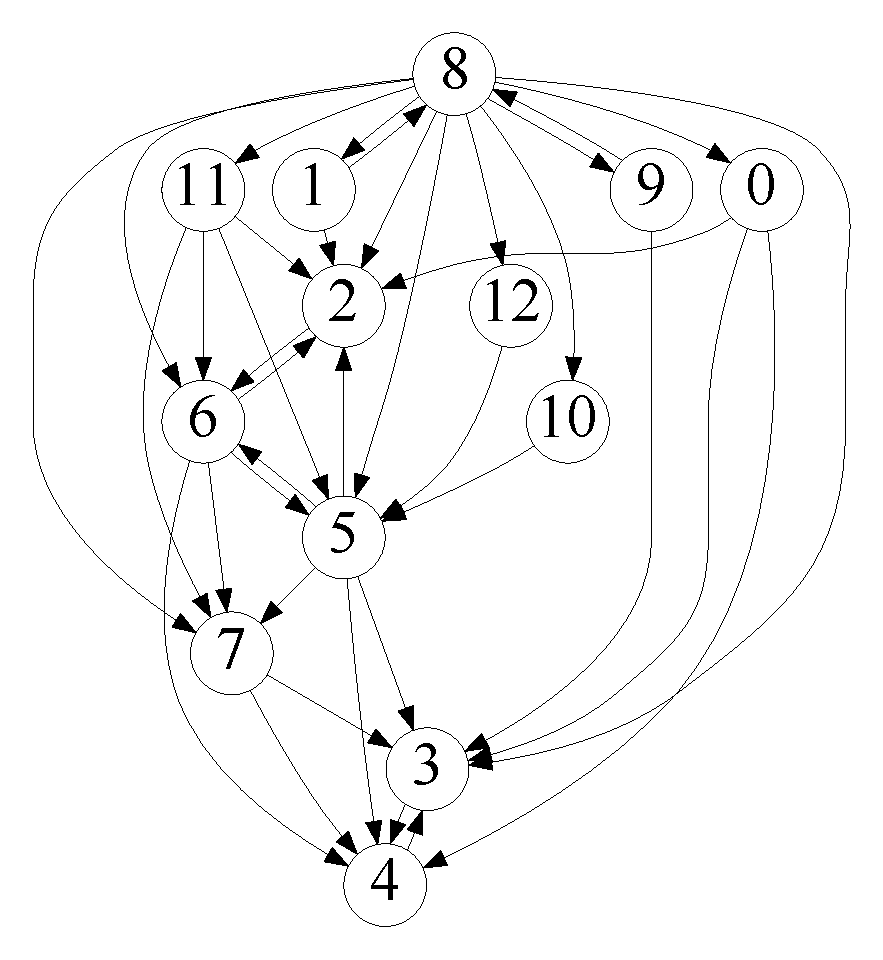
\includegraphics[width=\textwidth]{./alg_fig/simple-g0}}
		%     \vspace{-2em}
	\end{minipage}
	\begin{minipage}[b]{0.19\linewidth}
		\centering
		\subcaptionbox{add 5 to FVS\label{fig:simple:g2}}
		{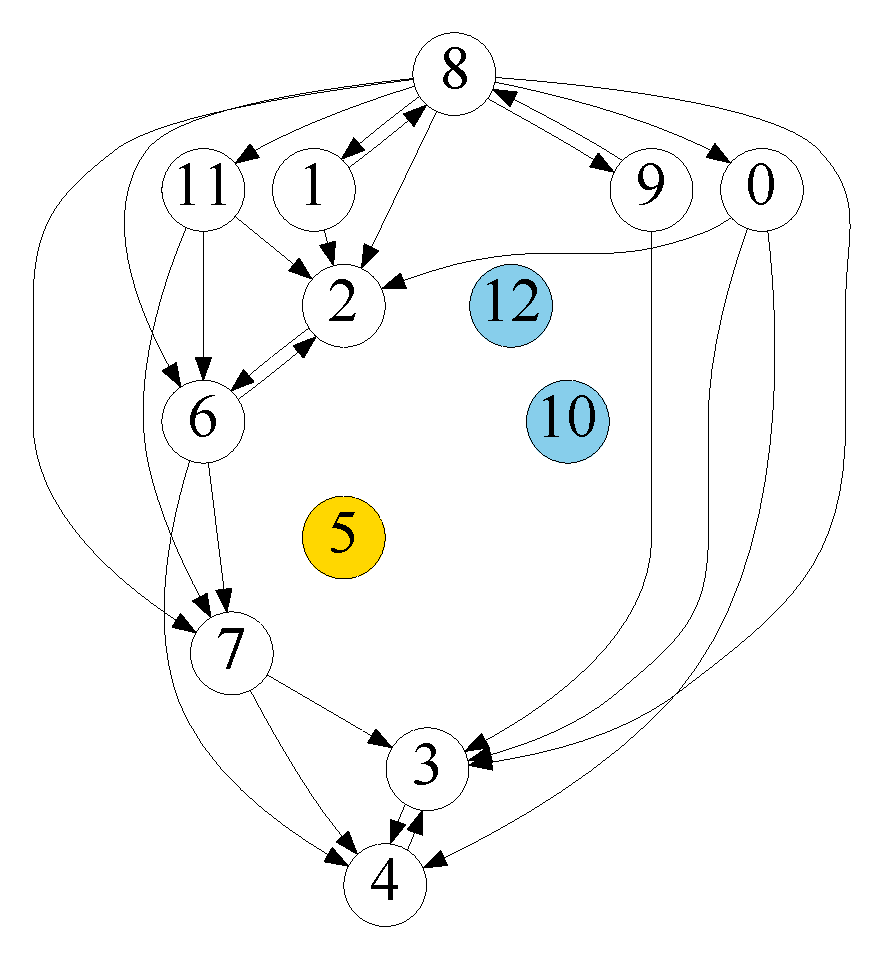
\includegraphics[width=\textwidth]{./alg_fig/simple-g2}}
		%    \vspace{-2em}
	\end{minipage}
	\begin{minipage}[b]{0.19\linewidth}
		\centering
		\subcaptionbox{add 8 to FVS\label{fig:simple:g4}}
		{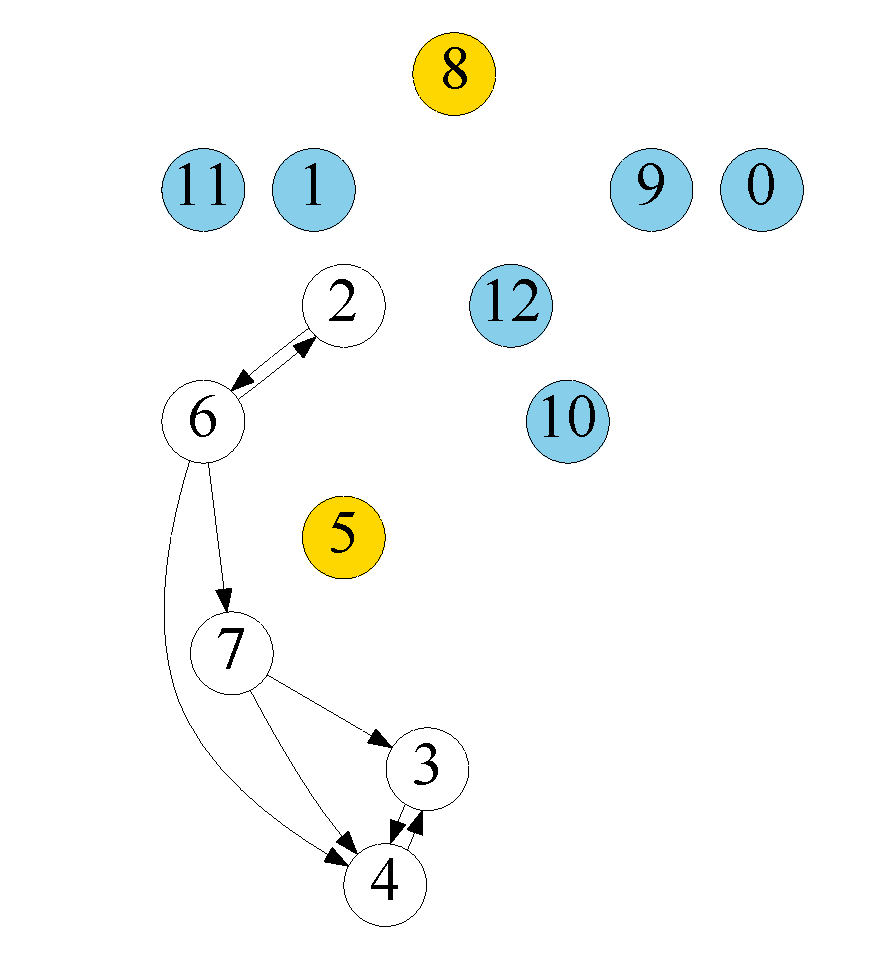
\includegraphics[width=\textwidth]{./alg_fig/simple-g4}}
		%       \vspace{-2em}
	\end{minipage}
	\begin{minipage}[b]{0.19\linewidth}
		\centering
		\subcaptionbox{add 6 to FVS\label{fig:simple:g6}}
		{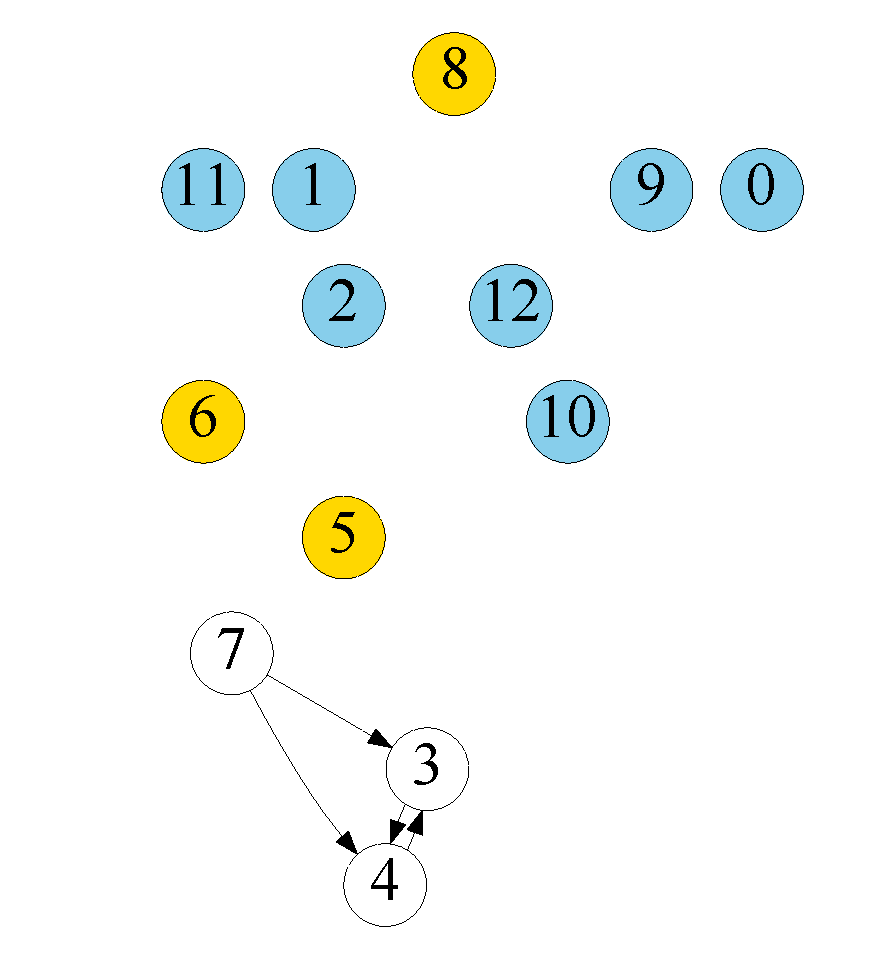
\includegraphics[width=\textwidth]{./alg_fig/simple-g6}}
		%      \vspace{-2em}
	\end{minipage}                  
	\begin{minipage}[b]{0.19\linewidth}
		\centering
		\subcaptionbox{add 3 to FVS\label{fig:simple:g8}}
		{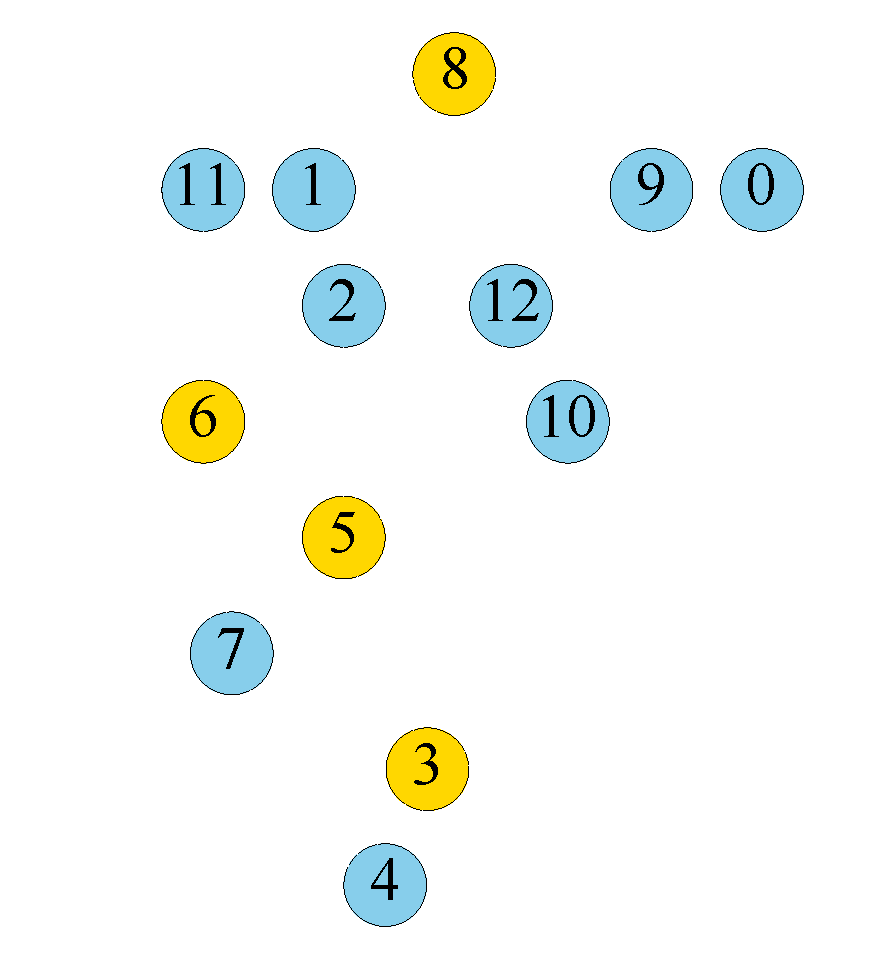
\includegraphics[width=\textwidth]{./alg_fig/simple-g8}}
		%     \vspace{-2em}
	\end{minipage}
	%\vspace{-1em}             
	\caption{An example of the sort-based greedy algorithm using \texttt{prod-degree} policy and multi factor 1. Blue nodes are trimmed during the algorithm, and yellow nodes form the FVS.}
	\label{fig:simple}               
	%\vspace{-1em}    	
\end{figure*}

{\bf Example (Continued).} Figure~\ref{fig:simple} shows the same example using the sort-based greedy algorithm, with $k = 1$. After the first sort, we add Node 5 to the FVS since it has the highest product of in-degree and out-degree. After eliminating Node 5, Nodes 10 and 12 have only incoming edges, and get trimmed (Figure~\ref{fig:simple:g2}). We sort the remaining nodes. This time, we add Node 8 to the FVS, and trim Nodes 0, 1, 9, 11 (Figure~\ref{fig:simple:g4}). We repeat this process with the remaining nodes until the graph is empty. This yields a FVS consisting of Nodes 3, 5, 6, and 8 (Figure~\ref{fig:simple:g8}), which contains one more vertex than the FVS we obtained with the SCC-based algorithm.

{\bf Hybrid Algorithm.}
%\subsubsection{Hybrid algorithm} 
We can combine the SCC-based greedy algorithm and the precise brute-force FVS search into a \emph{hybrid algorithm}. The algorithm is similar to the SCC-based greedy algorithm but runs a precise, brute-force FVS search whenever it can afford to. Instead of processing all SCCs via the $GreedyComponent$ subroutine (lines 5-7 of Algorithm~\ref{alg:scc}), it runs the precise search when processing SCCs that are smaller than a certain \emph{threshold}, and the greedy subroutine $GreedyComponent$ on SCCs that are larger than the threshold. Adjusting the threshold allows us to trade off precision versus runtime.

\subsection{Policies}
\label{subsec:validator_reordering:policy}
Policies are of utmost importance for our algorithms. Recall that a policy is a ranking function on vertices of the graph, and a good policy ranks vertices which are likely to be in a desirable FVS highly. 

% minimize number of conflicts
We first discuss policies that aim at minimizing the number of conflicts, i.e., the size of the FVS. The simplest such policy is \texttt{random} that assigns all nodes random rankings. Alternatively, we can rank nodes using degree-based heuristics, based on the intuition that the removal of a node will break many cycles if the node is high in some measurement of its graph degree. Such heuristics have  been shown to work well for FVS computation~\cite{cutello2015targeting}. For example, the policy \texttt{max-degree} chooses the node with the largest degree (either in-degree or out-degree), \texttt{sum-degree} chooses the node with the largest total degree (in-degree plus out-degree), and \texttt{prod-degree} chooses the node with the largest product of in-degree and out-degree. 
% minimize tail latency
More sophisticated policies are possible if the system is optimizing for a metric beyond maximizing the number of commits. For example, we may want to bound the transactions' tail latency; we can do that by incorporating latency information in our policies. We can rank transactions based on how many times they have been aborted and restarted; thus, transactions that have been restarted many times are much less likely to enter the FVS and have a higher chance of committing. Alternatively, we can also devise policies that combine the information about a transaction's number of restarts and its graph degree. For example, we can compute the ranking of a vertex as the product of its in-degree and out-degree divided by an exponential function of the number of restarts of the corresponding transaction. 
% help with transactions with monetary value
%\eat{We can also devise policies that handle hard transactions. In many workloads some transactions are naturally more prone to conflicts, e.g., those that access many objects and/or ``hot'' objects. If we use graph degree based policies, such transactions are likely to be included in the FVS and aborted repeatedly. To avoid starvation, we can adjust our policies to increase the probability that these transactions can commit. For example, we can approximate the ``hardness'' of a transaction by the size of its read and write sets and include that as a weighting factor in the policy.}
In business applications, the monetary value of different transactions varies. Optimizing for maximal monetary value, we can design policies that favor more valuable transactions. For example, we can customize the policy to always add a transaction with the lowest value to the FVS until the resulting dependency graph is acyclic.

%%%%%%%%%%%%%%%%%%%%%%%%%%%%%%%%%%%%%%%%%%%%%%%%%%%%%%%%%%%%%%%%%%%%%%
%%%%%%%%%%%  PARALLELISM
%%%%%%%%%%%%%%%%%%%%%%%%%%%%%%%%%%%%%%%%%%%%%%%%%%%%%%%%%%%%%%%%%%%%%%


\section{Parallelism}
\label{sec:parallel}

\changed{
\subsection{Parallel Reordering at Validation}
}

\label{subsec:validator_reordering:parallel}
Since batching and reordering occur as part of the transaction execution, it can increase the overall transaction latency, 
resulting in a higher chance of conflicts. Thus, we introduce parallelism into validation wherever possible to reduce latency.
Recall that the validator first prepares a batch of transactions, then reorders them using one of our algorithms from Section \ref{sec:valbatching},  
and finally validates them and caches the resulting updates of transactions that commit.
 Each of these steps corresponds to a subcomponent in the validator. Parallelism across these components seems difficult since there are strict sequential dependencies among these components. In this section, we explain how we actually manage to parallelize execution within each component and then even across components.


Figure~\ref{fig:reorder:validator} shows the architecture of our parallel validator. The validator has three components: 
%through the use of pipelining, as well as within each component. 
The \emph{batch preparation component} receives transactions from the processor, packages them into batches, and sends batches to the \emph{transaction reordering component}. The transaction reordering component reorders the transactions using one of our algorithms from Section \ref{sec:valbatching}, and then sends a validation request to the \emph{transaction validation component}. The transaction validation component takes a batch of ordered 
transactions
and validates them against the latest validator cache. It also updates the validator cache with the updates from transactions that have passed the validation. 

{\bf Parallelism Within Each Component.}
First, we can introduce parallelism into each of the components. In batch preparation, multiple threads can package transactions into batches. We can either assign each processor to send its validation request to a specific batch preparation thread, or we can create a consumer-producer queue to connect the processors and the batch preparation threads. In transaction reordering, multiple threads can consume reordering requests from the batch preparation threads, and reorder batches of transactions concurrently. Since the batches are not ordered yet in the reordering stage (although transactions within each batch are now ordered), the threads can send the processed batches to the validation component in any order. At the validation component, the batches are processed in order and validated against all previously committed transactions. 
%We cannot simply validate each individual transaction on a different thread since transactions come from different batches can conflict with each other. 
Within an ordered batch, since the transactions are already serialized by the ordering produced from the reordering component, the only source of conflicts is from all the transactions committed prior to the batch. Thus the validation of all transactions within a batch can be processed in parallel. Since conflicts can happen across batch boundaries, processing a new batch can only start after all the transactions in the previous batch have been validated. The updates from committed transactions in a batch are applied to the validator cache in serialization order at the end of the processing of the batch. Alternatively, we can use partitioned parallelism within a batch: We partition the key space and break a transaction into smaller pieces, one for each piece of the key space, and we assign different threads to validate transaction pieces in different partitions. This is analogous to the design of a partitioned validator in~\cite{ding2015centiman}.


% Pipeline parallelism
{\bf Parallelism Across Components.}
We can further increase parallelism by running the three validator components in parallel using pipelined parallelism, 
with each component working on a different batch in parallel. The batches then shift from component to component through the validator.

{\bf A Further Refinement: Pre-Validation.} As we mentioned in Section~\ref{subsec:validator_reordering}, prior to reordering, we can remove transactions that are not viable, i.e., conflicting with previously committed transactions. While this \emph{pre-validation} adds an additional validation for transactions on top of the final validation which serializes them, it reduces the number of transactions to reorder and the reordering algorithm runs faster. In our experiments, we observed that the reordering component was by a large factor the bottleneck piece, and eliminating non-viable transactions with pre-validation significantly improved performance. Thus, after batch creation, we first pre-validate the batch, reorder the remaining transactions, and then perform a second and final validation against the current database state.

We illustrate this design in Figure \ref{fig:reorder:validator}. The bottom row shows the set of database snapshots, one after each batch of transactions that has been validated. Consider a batch $B$. With pre-validation, $B$ will get validated against a ``stale'' database state $S$. Those transactions within batch $B$ that did not abort during pre-validation were then re-ordered and validated a second time in the transaction validation component against the ``correct'' database state $S'$. Since $S'$ now reflects all the updates from transactions that committed while $B$ was in the reordering component, transactions in $B$ can show conflicts during the final validation even through they were once already pre-validated in the reordering component.

%. We denote a database snapshot as $S_k$, where transactions whose timestamps are less or equal to $k$ have been committed as of this snapshot. In the reordering subcomponent, a batch of transactions $B$ is validated against the latest database snapshot $S_m$. The remaining transactions after pre-filtering are reordered as a batch $B'$ and sent to the validation\eat{ subcomponent}. $B'$ is again validated against the current database snapshot $S_n$. Since the validation subcomponent can be validating uncommitted transactions while $B$ is being processed at the reordering subcomponent, when $B'$ arrives at the validation\eat{ subcomponent},  we may have $n\geq m$. Thus, transactions in $B'$ can still abort due to conflicts with previously committed transactions in $S_n$.

% Parallelism in each subcomponent.

\begin{figure}[t]
	\centering
	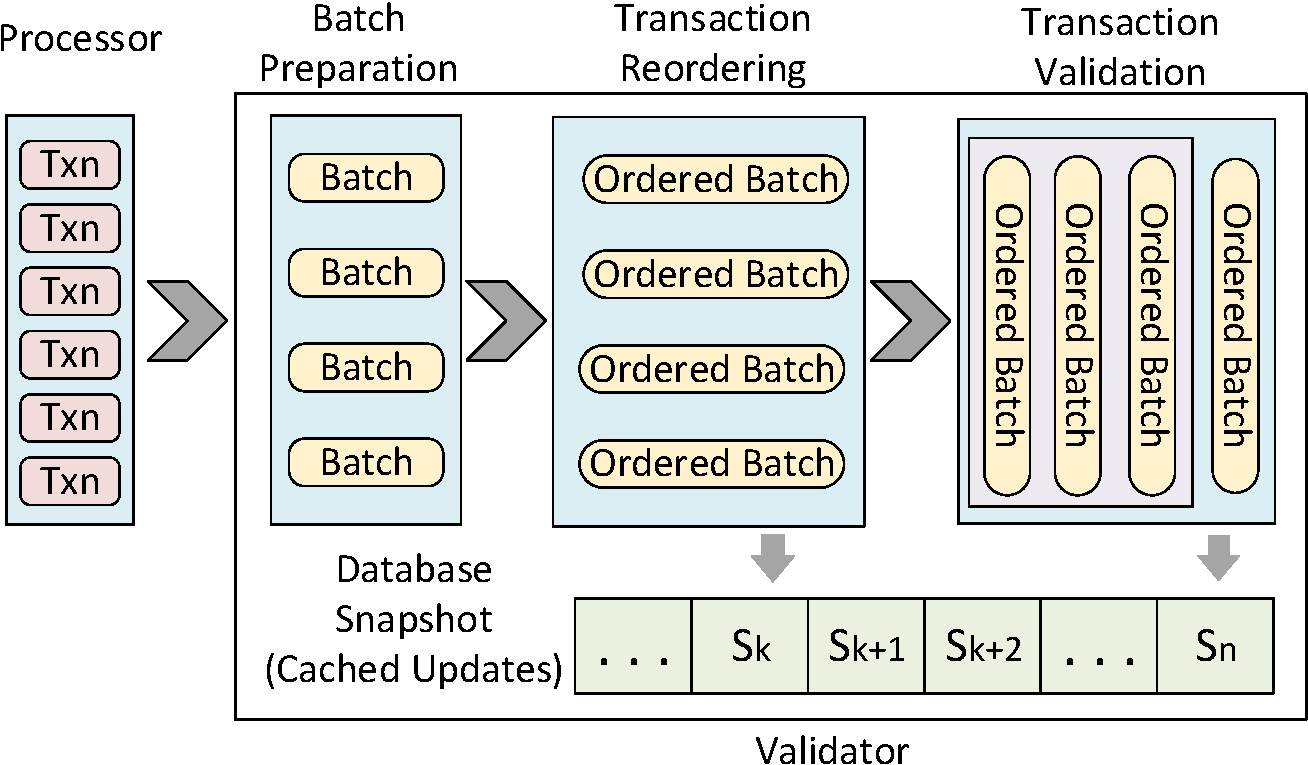
\includegraphics[width=1\columnwidth]{./figures/validator}
	\vspace{-2em}
	\caption{The architecture of parallel validator. It is decoupled into three subcomponents for pipeline parallelism: batch preparation, transaction reordering, and transaction validation. Each subcomponent can be further parallelized.}
	\vspace{-1em}
	\label{fig:reorder:validator}
\end{figure}

\changed{
\subsection{Synchronous Multi-Threaded Architecture}
\label{subsec:reorder_thread}
Many recent OLTP kernels use a decentralized architecture~\cite{lim2017cicada, tu2013speedy}, where there is no centralized thread for validation or storage access. Each transaction is scheduled to a dedicated thread and processed by this thread synchronously for its entire life time. Since a transaction is executed synchronously, a transaction can only conflict with transactions executed by other threads. 

In such architectures, while batching operations across transactions does not apply, we can reorder the transactions to reduce inter-thread conflicts with better data caching as a side-effect.

Intuitively, for a batch of incoming transactions, we schedule the transactions with conflicts to execute on the same thread to reduce conflicts among different threads. Because conflicting transactions access the same data, reordering also improves caching.

We adapt our reordering algorithm for synchronous multi-threaded architectures with a thread-aware policy to schedule transactions thread by thread. We initialize the weight of the transaction to be the number of read-write conflicts it has among a batch of incoming transactions. For each thread, we first pick the transaction with the most conflicts from the remaining transactions. Iteratively, the policy updates the weight of each remaining transaction to the number of transactions it conflicts with in this thread and picks the next transaction with the highest weight, breaking ties by the number of objects a transaction shares with the transactions already scheduled to this thread.
}
%%%%%%%%%%%%%%%%%%%%%%%%%%%%%%%%%%%%%%%%%%%%%%%%%%%%%%%%%%%%%%%%%%%%%%
%%%%%%%%%%%  PARALLELISM
%%%%%%%%%%%%%%%%%%%%%%%%%%%%%%%%%%%%%%%%%%%%%%%%%%%%%%%%%%%%%%%%%%%%%%


\subsection{Parallelism}
\label{sec:parallel}
\label{sec:validator_reordering:parallel}

%\changed{
%\subsection{Parallel Reordering at Validation}
%}

Since batching and reordering occur during transaction execution, they can increase transaction latency, 
resulting in a higher chance of conflicts. Thus, we introduce parallelism into validation.
Recall that the validator first prepares a batch of transactions, then reorders them,  
and finally validates them and caches the resulting updates of transactions that commit.
 Each step corresponds to a subcomponent in the validator. Parallelism across these components seems difficult since there are strict sequential dependencies among them. We first explain how to parallelize execution within each component and then even across components.


Figure~\ref{fig:reorder:validator} shows the architecture of our parallel validator, including three components: 
%through the use of pipelining, as well as within each component. 
The \emph{batch preparation component} receives transactions from the processor, packages them into batches, and sends the batches to the \emph{transaction reordering component}. The transaction reordering component reorders the transactions, and then sends a validation request to the \emph{transaction validation component}. The transaction validation component takes a batch of ordered 
transactions
and validates them against the latest validator cache. It also updates the validator cache with the updates from transactions that pass the validation. 

{\bf Parallelism within a component.}
\cut{First, we can introduce parallelism into each component. }In batch preparation, multiple threads can package transactions into batches. We can either assign each processor to send its validation request to a specific batch preparation thread, or we can create a consumer-producer queue to connect the processors and the batch preparation threads. In transaction reordering, multiple threads can consume reordering requests from the batch preparation threads, and reorder batches of transactions concurrently. Since the batches are not ordered yet in the reordering stage (although transactions within each batch are now ordered), the threads can send the processed batches to the validation component in any order. At the validation component, the batches are processed serially and validated against all previously committed transactions. 
%We cannot simply validate each individual transaction on a different thread since transactions come from different batches can conflict with each other. 
Within an ordered batch, since the transactions are already serialized \cut{by the ordering produced from }by the reordering component, the only source of conflicts is from \cut{all the} transactions committed prior to the batch. Thus, \cut{the validation of all }transactions within a batch can be validated in parallel. Since conflicts can happen across batches, a new batch can only be processed after transactions from previous batches have been validated. Updates from committed transactions in a batch are applied to the validator cache in serialization order at the end of the processing of the batch. We can further partition the key space to parallelize within a batch\eat{: We partition the key space and break a transaction into smaller pieces, one for each piece of the key space, and we assign different threads to validate transaction pieces in different partitions. This is }, which is similar to the design of a partitioned validator~\cite{ding2015centiman}.


% Pipeline parallelism
{\bf Parallelism across components.}
We can further increase parallelism by running the three validator components with pipelined parallelism, 
with each component working on a different batch in parallel. The batches then shift from one component to the next component in the validator.

{\bf A further refinement: Pre-validation.} As mentioned in Section~\ref{subsec:validator_reordering}, prior to reordering, we can remove non-viable transactions, i.e., transactions that conflict with previously committed transactions. While this \emph{pre-validation} adds an additional validation for transactions on top of the final validation which serializes them, it reduces the number of transactions to reorder and the reordering algorithm runs faster. Empirically, we observe that the reordering component is the bottleneck piece, and removing non-viable transactions with pre-validation significantly improves performance. Thus, after batch creation, we first pre-validate the batch, reorder the remaining transactions, and then perform a second and final validation against the current database state.

In Figure \ref{fig:reorder:validator}, the bottom row shows a set of database snapshots, each after a batch of transactions that has been validated. With pre-validation, a batch $B$ will get validated against a ``stale'' database state $S$. Those transactions within batch $B$ that have passed the pre-validation are then re-ordered and validated a second time in the transaction validation component against the ``correct'' database state $S'$. Since $S'$ now reflects all the updates from transactions committed after $S$ while $B$ is in the reordering component, transactions in $B$ can still show additional conflicts during the final validation.

%. We denote a database snapshot as $S_k$, where transactions whose timestamps are less or equal to $k$ have been committed as of this snapshot. In the reordering subcomponent, a batch of transactions $B$ is validated against the latest database snapshot $S_m$. The remaining transactions after pre-filtering are reordered as a batch $B'$ and sent to the validation\eat{ subcomponent}. $B'$ is again validated against the current database snapshot $S_n$. Since the validation subcomponent can be validating uncommitted transactions while $B$ is being processed at the reordering subcomponent, when $B'$ arrives at the validation\eat{ subcomponent},  we may have $n\geq m$. Thus, transactions in $B'$ can still abort due to conflicts with previously committed transactions in $S_n$.

% Parallelism in each subcomponent.


\section{Evaluation}\label{sec:experiments}
In our experimental evaluation, we wanted to understand the effect of batching and reordering at storage and validator, the performance of our validator reordering algorithms and policies, parallelizing transaction reordering at validator, and the impact of system configuration parameters. In particular, we asked the following questions:
\begin{enumerate}
\item\vspace{-.8em} How well do our validator reordering algorithms from Section~\ref{subsec:validator_reordering:algorithm} perform? How does batching and reordering at validator using these algorithms affect the end-to-end system performance?
\item\vspace{-.8em} How does the batch size impact performance? 
\item\vspace{-.8em} How does parallel reordering impact the system performance?
\item\vspace{-.8em} How does storage and validator batching and reordering affect the system performance?
\item\vspace{-.8em} How do the different policies presented in Section~\ref{subsec:validator_reordering:policy} impact the system performance?
\item\vspace{-.8em} How does batching and reordering perform on real workloads?
\end{enumerate}

\subsection{Experimental Setup}
\label{subsec:experiment:implementation}

%Our system architecture consists of four components: a transaction generator, a processor thread, a storage thread, and a validator thread. The threads communicate through queues of requests; that is, there is a generator queue, a processor queue, a storage queue, and a validator queue.

Our system architecture consists of four components: transaction generation, a processor, storage, and validation. The components communicate through consumer-producer queues.

The transaction generator continuously produces new transactions until the system reaches the maximum permitted concurrency level. The processor multiplexes transactions as a transaction coordinator, receives transaction requests from the transaction generator, sends read/write requests to the storage, sends validation requests to the validator, and replies to the transaction generator. It also restarts aborted transactions; thus, it only communicates commit decisions to the transaction generator. 
The storage continuously processes read and write requests. When storage batching is enabled, it buffers a batch of requests. When processing a batch, it uses the optimal strategy that we discussed in Section~\ref{sec:overview}: It first executes all the write requests in the batch (discarding a write if a newer version exists in the storage), and then all the read requests. 

% validator
The validator performs backward validation. For every transaction, a validation request consists of the keys and versions of its reads and the keys of its writes. The validator caches the write keys of committed transactions in an in-memory hash table, until these writes are overwritten by later updates. When batching is enabled, the validator collects the requests into a batch as they arrive, and runs one of the algorithms from Section~\ref{sec:validator_reordering} to determine a serialization order. Every transaction that passes validation is assigned an integer \emph{commit timestamp}, which corresponds to the version number of the updates it will install in storage. 

% Validator
We have further decoupled the validator component into four subcomponents as described in Section~\ref{subsec:validator_reordering:parallel}. A batch preparation worker receives validation requests from the processor, packages transactions into batches, and queues them for reordering. A transaction reordering worker takes a batch from the queue, pre-validates and filters the transactions in the batch against the validator cache, reorders the transactions, and queues the ordered transactions as a new batch for validation. A validation worker takes a batch from the queue, serializes the transactions, and validates the transactions against the current validator cache, and sends committed transactions to the cache update worker. The cache update worker finally applies updates to the validator cache based on the transaction serialization order. 

% Details of validator implementation.
By default, the validator uses the sort-based greedy algorithm with the \texttt{prod-degree} policy and multi factor 2. To process a batch, we create a dependency graph as described in Section~\ref{subsec:validator_reordering:algorithm}. We have empirically determined that validator reordering is not beneficial if the dependency graph is very dense, as there are fewer opportunities for conflict reduction. Therefore, we heuristically set a limit on the size of the dependency graph. Once we detect that the number of edges has hit this limit during the construction of the dependency graph, we discard the graph and validate the transactions without reordering. 

% Parallelization.
We have parallelized the transaction generation, the storage, and the transaction reordering at the validator. By default, two transaction generators populate the transactions concurrently to supply sufficient load. Two storage workers concurrently process reads and writes, and the writes are applied based on its data versioning as described in Section~\ref{sec:overview}. In the validator, we first introduced pipeline parallelism by processing different subcomponents concurrently. Since we observed that transaction reordering is heavier weight as compared to other subcomponents, we increased its capacity by multi-threading. We used four transaction reordering workers by default.

% Hard ware and data population.
Our system is implemented in Java. All the experiments run on a machine with Intel Xeon E5-2630 CPU @2.20GHz and 16GB RAM. We use a key-value model for the storage, which we implement as an in-memory hash table. In our micro benchmark, we populate the database with 100K objects, each with an 8-byte key. The values are left null as they are not relevant to our evaluation. We generate a transactional workload where each transaction reads 5 objects and writes to 5 objects, with of the reads and one of the writes on the same object. The reads and writes are drawn from a Zipfian distribution, implemented based on the standard model by Gray et al.~\cite{gray1994quickly}. We limit the concurrency level to 300, i.e., at any time there are at most 300 live transactions in the system. The default batch size is 40 for both storage and validator.

% baseline
The baseline configuration represents the system running with both storage and validator batching turned off. We add a batch mode to separate the effect of batching and reordering. In the batch mode, batching is enabled at both storage and validator, but no reordering is performed. The batch mode can benefit from better caching with tighter loops in the processing. 

% other configuration
\eat{The validator uses the sort-based greedy algorithm with the \texttt{prod-degree} policy and multi factor 2.} 

% Misc
All our experimental figures show the averages of 10 runs, each lasting for 60 seconds in between a 10-second warm-up and a 10-second cool-down time. The standard deviation was not significant in any of the experiments, so we omit the error bars for clarity of presentation. We report the good throughput (the number committed transactions per second), the average latency, and the percentile latency.


% *******************
% * Figures
% *******************
\begin{figure*}[t]
    \centering
    \begin{minipage}[b]{0.32\linewidth}
        \centering
        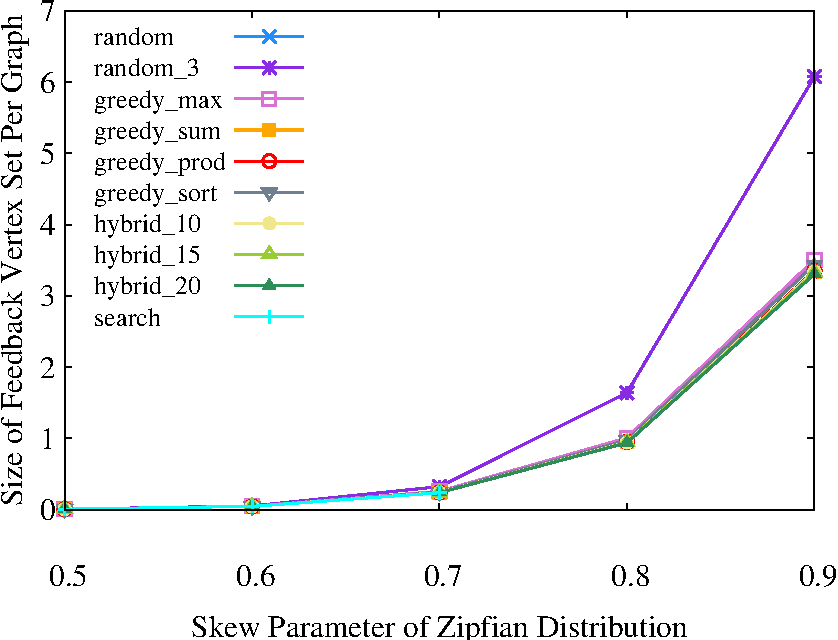
\includegraphics[width=\textwidth]{./exp_fig/fvs/fvs}
        \vspace{-2em}
        \caption{Size of FVS per graph with different algorithms}
        \label{fig:fvs:fvs}
    \end{minipage}
    \begin{minipage}[b]{0.32\linewidth}
        \centering
        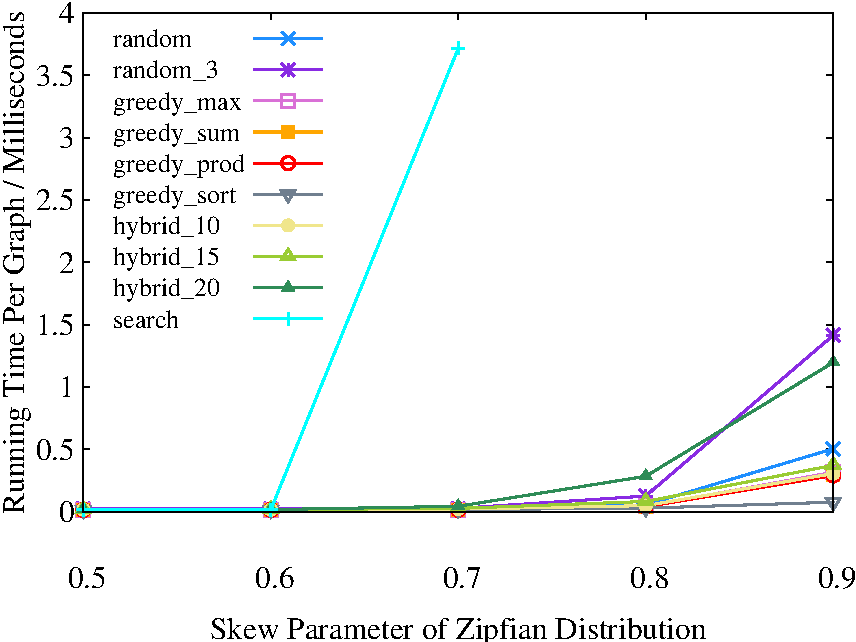
\includegraphics[width=\textwidth]{./exp_fig/fvs/latency}
        \vspace{-2em}
        \caption{Running time of finding FVS with different algorithms}
        \label{fig:fvs:latency}
    \end{minipage}
    \begin{minipage}[b]{0.32\linewidth}
        \centering
        \includegraphics[width=\textwidth]{./exp_fig/greedy/tps}
        \vspace{-2em}
        \caption{Throughput with SCC-based and sort-based greedy algorithms}
        \label{fig:greedy:tps}
    \end{minipage}
    \vspace{-1em}
\end{figure*}

\begin{figure*}[t]
    \centering
    \begin{minipage}[b]{0.32\linewidth}
	\centering
	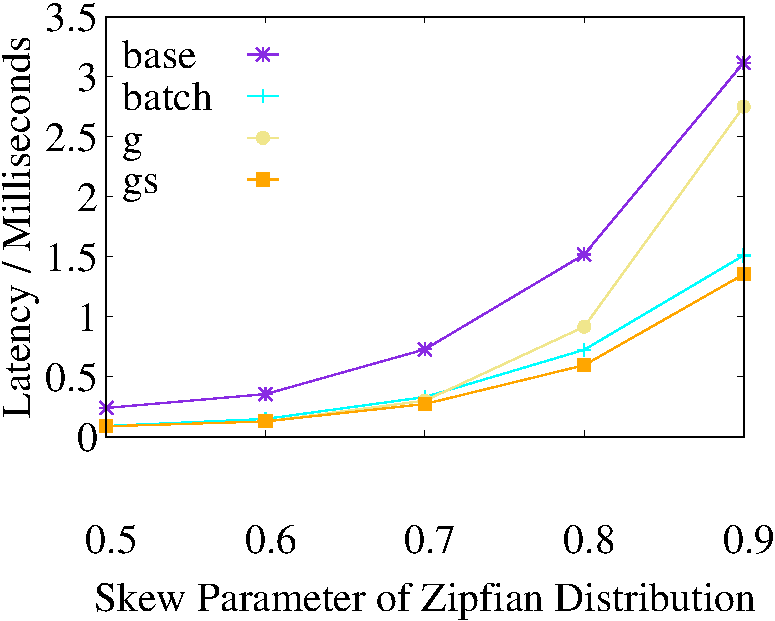
\includegraphics[width=\textwidth]{./exp_fig/greedy/latency}
	\vspace{-2em}
	\caption{Average latency for greedy algorithms}
	\label{fig:greedy:latency}
	\end{minipage}
    \begin{minipage}[b]{0.32\linewidth}
        \centering
        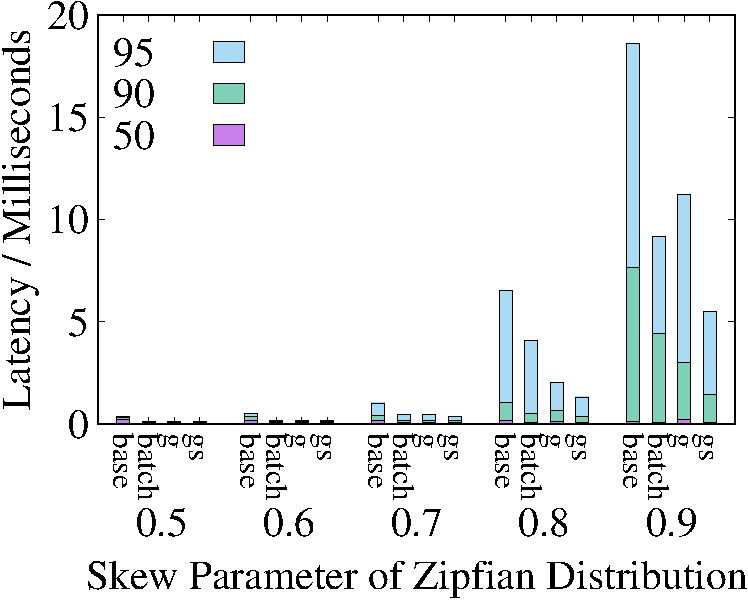
\includegraphics[width=\textwidth]{./exp_fig/greedy/percent95_latency}
        \vspace{-2em}
        \caption{Percentile latency for greedy algorithms}
        \label{fig:greedy:p95}
    \end{minipage}
    \begin{minipage}[b]{0.32\linewidth}
            \centering
            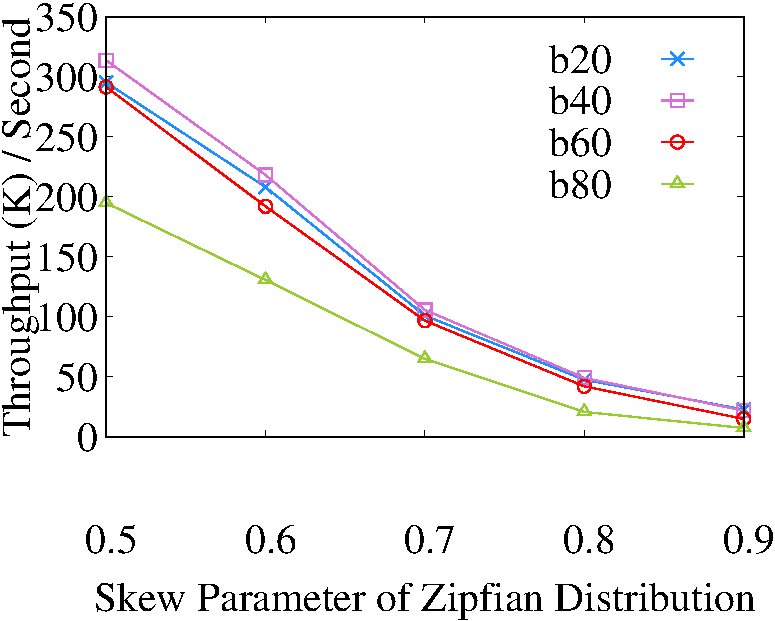
\includegraphics[width=\textwidth]{./exp_fig/bsize/tps}
            \vspace{-2em}
            \caption{Throughput with various batch sizes}
            \label{fig:bsize:tps}
    \end{minipage}    
    \vspace{-1em}
\end{figure*}

\begin{figure*}[t]
    \centering
    \begin{minipage}[b]{0.32\linewidth}
    	\centering
    	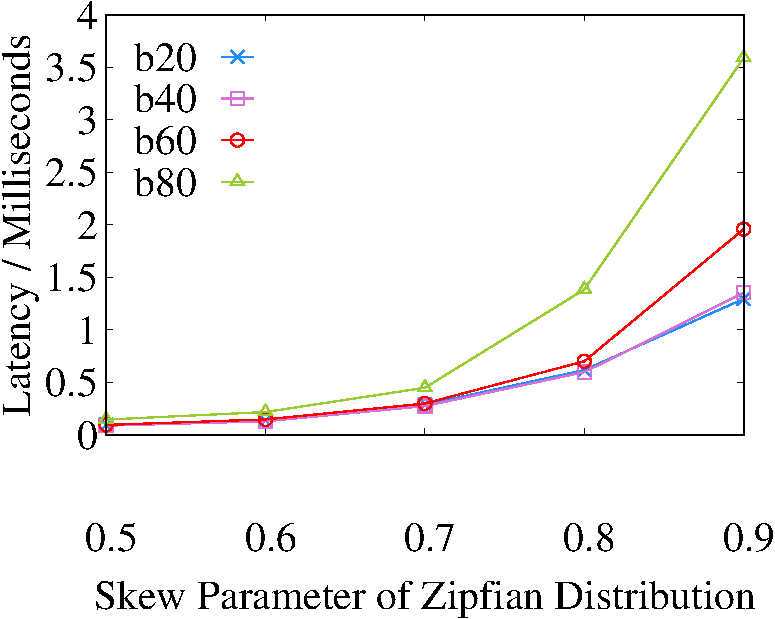
\includegraphics[width=\textwidth]{./exp_fig/bsize/latency}
    	\vspace{-2em}
    	\caption{Average latency with various batch sizes}
    	\label{fig:bsize:latency}
    \end{minipage}
    \begin{minipage}[b]{0.32\linewidth}
	\centering
	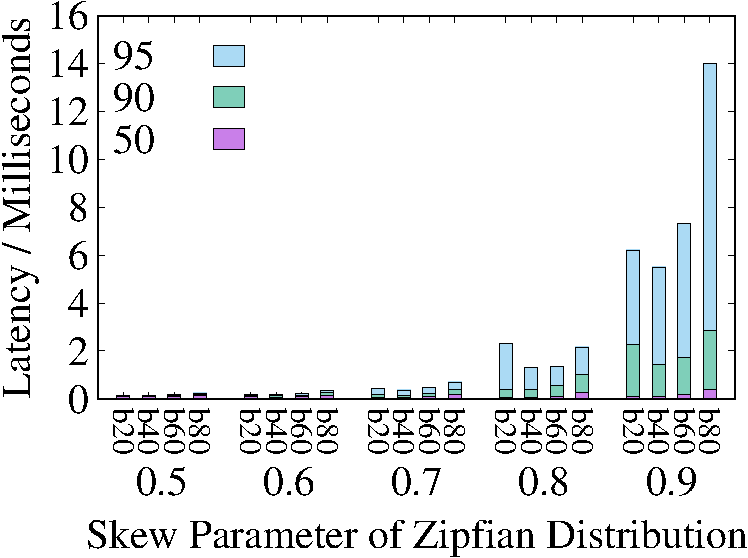
\includegraphics[width=\textwidth]{./exp_fig/bsize/percent95_latency}
	\vspace{-2em}
	\caption{Percentile latency with various batch sizes}
	\label{fig:bsize:p95}
	\end{minipage}
    \begin{minipage}[b]{0.32\linewidth}
	\centering
	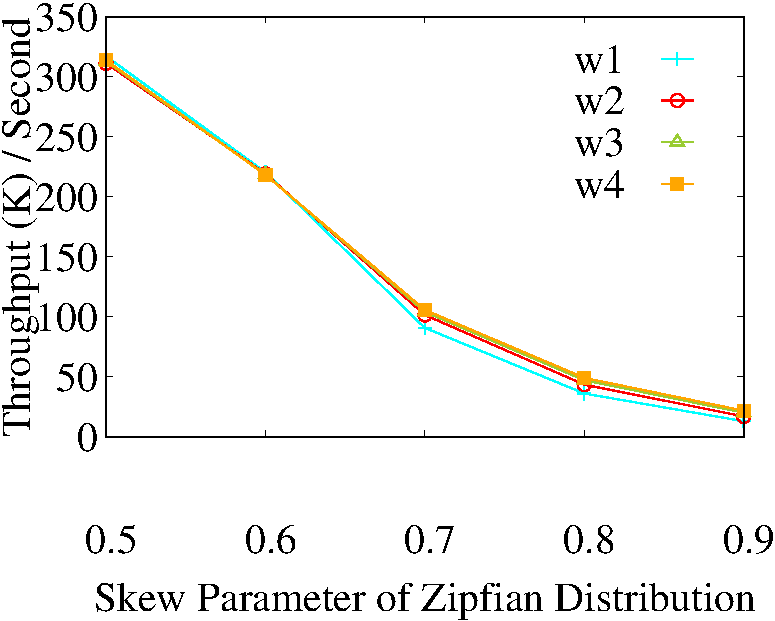
\includegraphics[width=\textwidth]{./exp_fig/reorder/tps}
	\vspace{-2em}
	\caption{Throughput with different number of reorder workers}
	\label{fig:reorder:tps}
	\end{minipage}    
    \vspace{-1em}
\end{figure*}

\begin{figure*}[t]
    \centering
	\begin{minipage}[b]{0.32\linewidth}
	\centering
	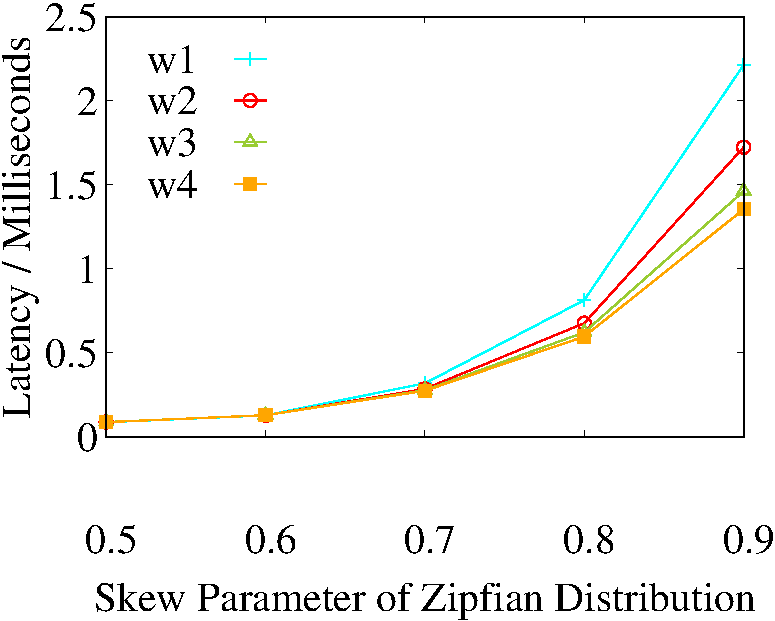
\includegraphics[width=\textwidth]{./exp_fig/reorder/latency}
	\vspace{-2em}
	\caption{Average latency with different number of reorder workers}
	\label{fig:reorder:latency}
	\end{minipage}    
    \begin{minipage}[b]{0.32\linewidth}
	\centering
	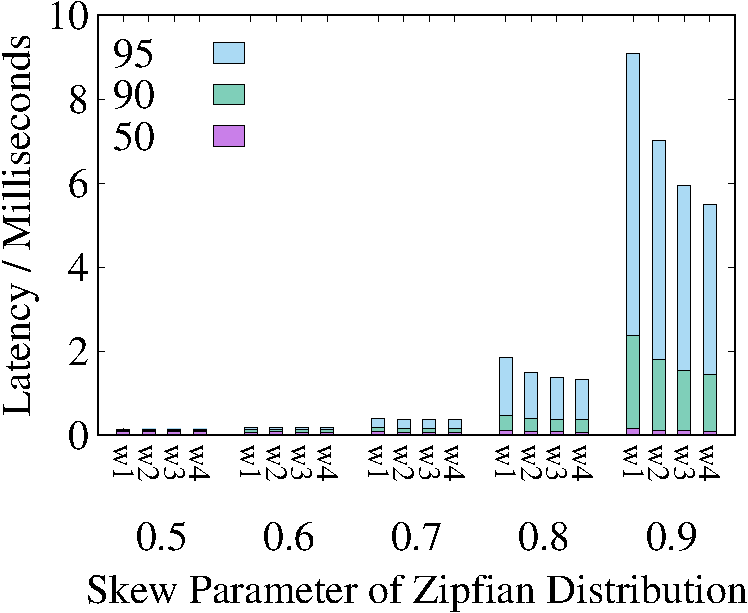
\includegraphics[width=\textwidth]{./exp_fig/reorder/percent95_latency}
	\vspace{-2em}
	\caption{Percentile latency with different number of reorder workers}
	\label{fig:reorder:p95}
	\end{minipage}    
	\begin{minipage}[b]{0.32\linewidth}
	\centering
	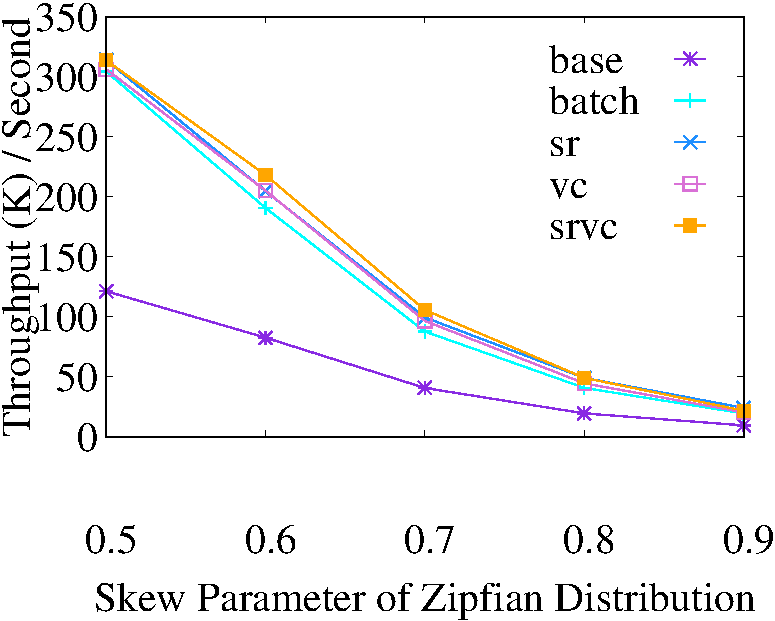
\includegraphics[width=\textwidth]{./exp_fig/basic/tps}
	\vspace{-2em}
	\caption{Throughput under workloads of Zipfian distribution}
	\label{fig:basic:tps}
	\end{minipage}    
    \vspace{-1em}
\end{figure*}

\begin{figure*}[t]
    \centering
    \begin{minipage}[b]{0.32\linewidth}
	\centering
	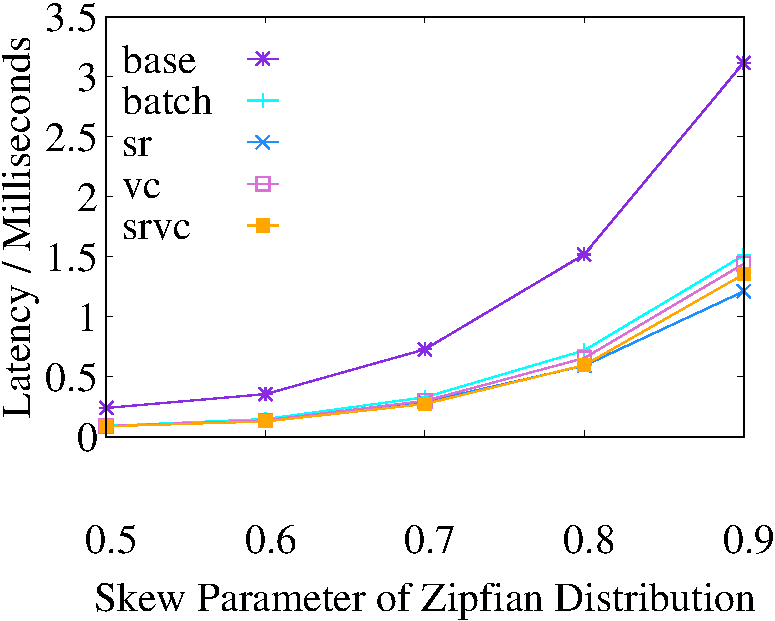
\includegraphics[width=\textwidth]{./exp_fig/basic/latency}
	\vspace{-2em}
	\caption{Average latency under workloads of Zipfian distribution}
	\label{fig:basic:latency}
	\end{minipage}
    \begin{minipage}[b]{0.32\linewidth}
	\centering
	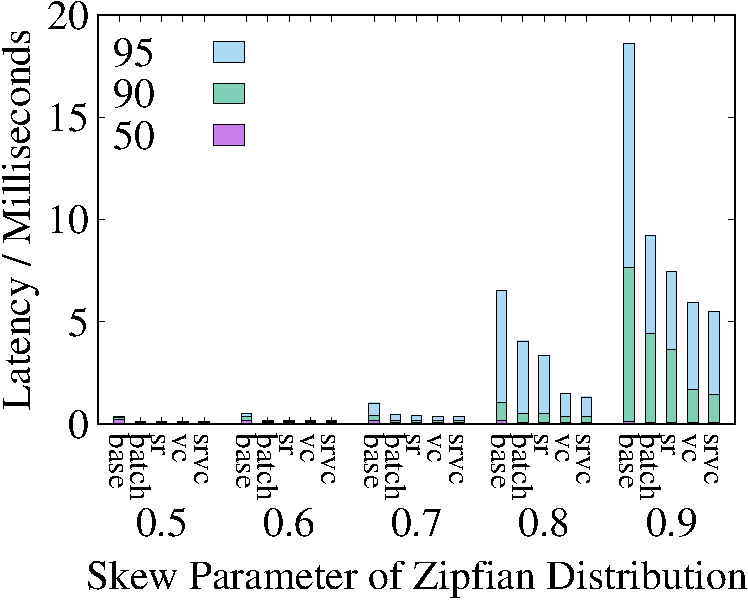
\includegraphics[width=\textwidth]{./exp_fig/basic/percent95_latency}
	\vspace{-2em}
	\caption{Percentile latency under workloads of Zipfian distribution}
	\label{fig:basic:p95}
	\end{minipage}
   \begin{minipage}[b]{0.32\linewidth}
	\centering
	\includegraphics[width=\textwidth]{{{./exp_fig/load/Z0.7_tps}}}
	\vspace{-2em}
	\caption{Throughput with micro benchmark (skew factor 0.7)}
	\label{fig:load_z0.7:tps}
	\end{minipage}
    \vspace{-1em}
\end{figure*}


% hard transactions
\begin{figure*}[t]
    \centering
	\begin{minipage}[b]{0.32\linewidth}
	\centering
	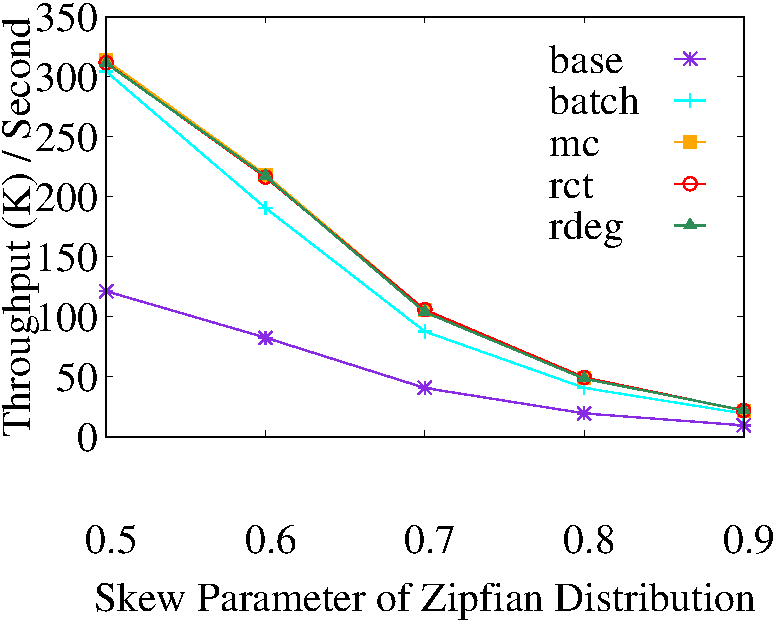
\includegraphics[width=\textwidth]{./exp_fig/restart/tps}
	\vspace{-2em}
	\caption{Throughput with tail latency optimized policies}
	\label{fig:restart:tps}
	\end{minipage}
    \begin{minipage}[b]{0.32\linewidth}
	\centering
	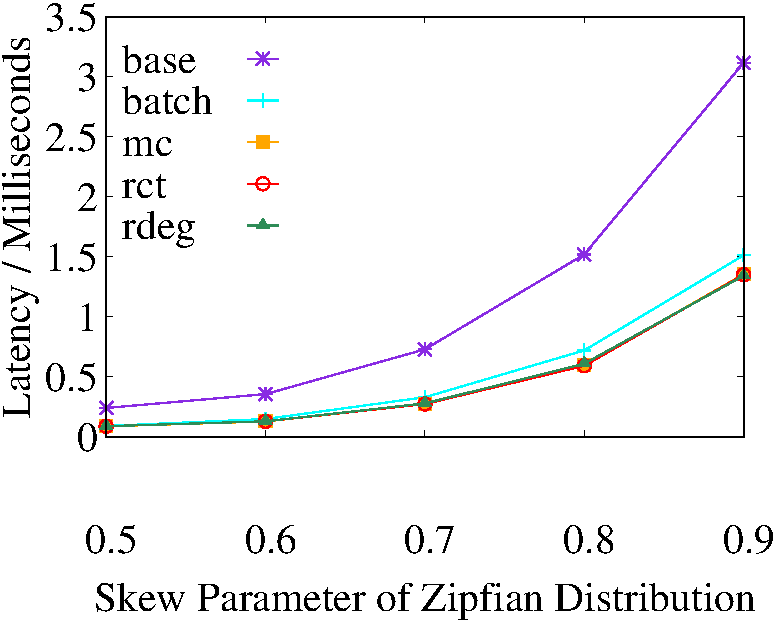
\includegraphics[width=\textwidth]{./exp_fig/restart/latency}
	\vspace{-2em}
	\caption{Average latency with tail latency optimized policies}
	\label{fig:restart:abort}
	\end{minipage}
    \begin{minipage}[b]{0.32\linewidth}
	\centering
	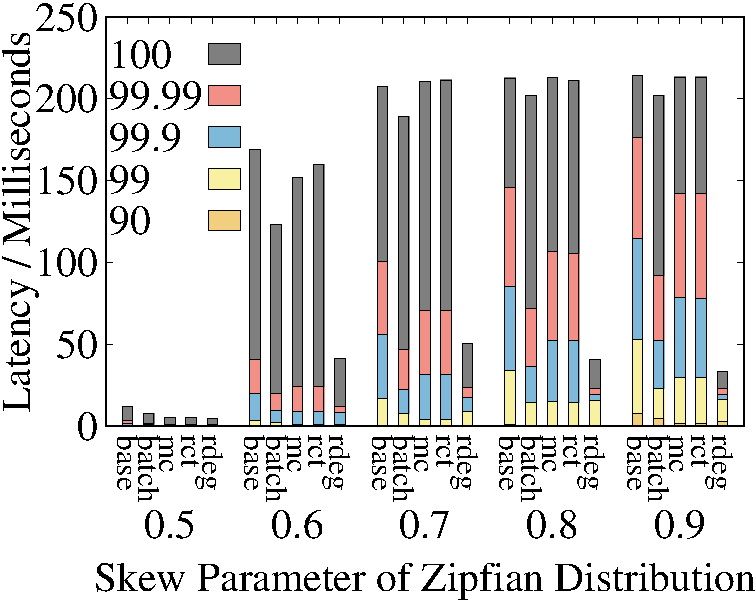
\includegraphics[width=\textwidth]{./exp_fig/restart/percent100_latency}
	\vspace{-2em}
	\caption{Percentile latency with tail latency optimized policies}
	\label{fig:restart:p100}
	\end{minipage}
%    \begin{minipage}[b]{0.32\linewidth}
%	\centering
%	\includegraphics[width=\textwidth]{{{./exp_fig/load/Z0.7_tps}}}
%	\vspace{-2em}
%	\caption{Throughput with micro benchmark (skew factor 0.7)}
%	\label{fig:load_z0.7:tps}
%	\end{minipage}
%   \begin{minipage}[b]{0.32\linewidth}
%	\centering
%	\includegraphics[width=\textwidth]{{{./exp_fig/load/Z0.8_tps}}}
%	\vspace{-2em}
%	\caption{Throughput with micro benchmark (skew factor 0.8)}
%	\label{fig:load_z0.8:tps}
%	\end{minipage}
	\vspace{-1em}
\end{figure*}


%\begin{figure*}[t]
%    \centering
%    \begin{minipage}[b]{0.32\linewidth}
%	\centering
%	\includegraphics[width=\textwidth]{{{./exp_fig/load/Z0.7_latency}}}
%	\vspace{-2em}
%	\caption{Average latency with micro benchmark (skew factor 0.7)}
%	\label{fig:load_z0.7:latency}
%	\end{minipage}
%\end{figure*}

%\begin{figure*}[t]
%    \centering
%    \begin{minipage}[b]{0.32\linewidth}
%	\centering
%	\includegraphics[width=\textwidth]{{{./exp_fig/small_bank/Z0.7_tps}}}
%	\vspace{-2em}
%	\caption{Throughput with Small Bank benchmark (skew factor 0.7)}
%	\label{fig:small_bank_z0.7:tps}
%	\end{minipage}
%   \begin{minipage}[b]{0.32\linewidth}
%       \centering
%        \includegraphics[width=\textwidth]{{{./exp_fig/small_bank/Z0.7_latency}}}
%        \vspace{-2em}
%        \caption{Average latency with Small Bank benchmark (skew factor 0.7)}
%        \label{fig:small_bank_z0.7:latency}
%    \end{minipage}
%	 \begin{minipage}[b]{0.32\linewidth}
%	\centering
%	\includegraphics[width=\textwidth]{{{./exp_fig/small_bank/Z0.8_tps}}}
%	\vspace{-2em}
%	\caption{Throughput with Small Bank benchmark (skew factor 0.8)}
%	\label{fig:small_bank_z0.8:tps}
%	\end{minipage}
%    \vspace{-1em}
%\end{figure*}

\begin{figure*}[t]
	\centering
%	\begin{minipage}[b]{0.32\linewidth}
%	\centering
%	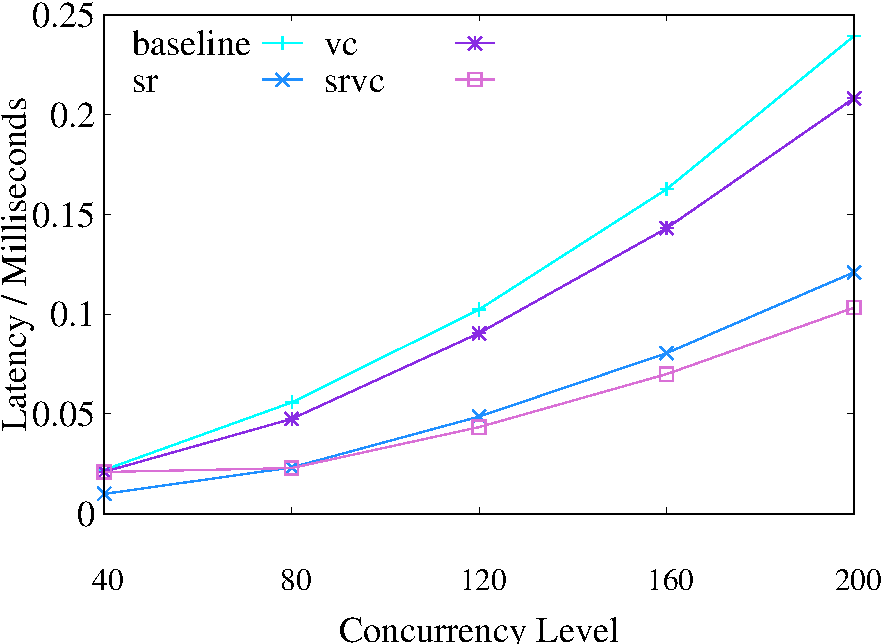
\includegraphics[width=\textwidth]{{{./exp_fig/load/Z0.8_latency}}}
%	\vspace{-2em}
%	\caption{Average latency with micro benchmark (skew factor 0.8)}
%	\label{fig:load_z0.8:latency}
%\end{minipage}
	 \begin{minipage}[b]{0.32\linewidth}
	\centering
	\includegraphics[width=\textwidth]{{{./exp_fig/small_bank/tps}}}
	\vspace{-2em}
	\caption{Throughput with Small Bank benchmark)}
	\label{fig:small_bank:tps}
	\end{minipage}
	\begin{minipage}[b]{0.32\linewidth}
	\centering
	\includegraphics[width=\textwidth]{{{./exp_fig/small_bank/latency}}}
	\vspace{-2em}
	\caption{Average latency with Small Bank benchmark}
	\label{fig:small_bank:latency}
	\end{minipage}
	\begin{minipage}[b]{0.32\linewidth}
	\centering
	\includegraphics[width=\textwidth]{{{./exp_fig/small_bank/percent95_latency}}}
	\vspace{-2em}
	\caption{Percentile latency with Small Bank benchmark}
	\label{fig:small_bank:p95}
	\end{minipage}
%	 \begin{minipage}[b]{0.32\linewidth}
%	\centering
%	\includegraphics[width=\textwidth]{{{./exp_fig/small_bank/Z0.9_tps}}}
%	\vspace{-2em}
%	\caption{Throughput with Small Bank benchmark (skew factor 0.9)}
%	\label{fig:small_bank_z0.9:tps}
%	\end{minipage}
%	\begin{minipage}[b]{0.32\linewidth}
%	\centering
%	\includegraphics[width=\textwidth]{{{./exp_fig/small_bank/Z0.9_latency}}}
%	\vspace{-2em}
%	\caption{Average latency with Small Bank benchmark (skew factor 0.9)}
%	\label{fig:small_bank_z0.9:latency}
%	\end{minipage}
%    \vspace{-1em}
\end{figure*}

% *******************
% * Experiments
% *******************
\subsection{Validator Reordering Algorithms}
\label{sec:exp_algorithms}
We first investigate the performance of the feedback vertex set algorithms from Section~\ref{subsec:validator_reordering:algorithm} 
%with a comparison of the raw performance of the algorithms, i.e., 
for their accuracy and running time. We run the algorithms on graphs constructed as described in Section~\ref{sec:valbatching}, using our micro benchmarks. 
%\eat{We first test the algorithms offline on the dependency graphs constructed at validator when running the system. Each dependency graph is constructed from a batch of transactions at validator, excluding non-viable transactions, i.e., we only use transactions that don't have inter-batch conflicts. We compare the averages of the size of the feedback vertex set and the running time per dependency graph.}
We test the SCC-based greedy algorithm with the \texttt{max-degree} ($greedy\_max$), \texttt{sum-degree} ($greedy\_sum$) and \texttt{prod-degree} policies ($greedy\_prod$). We also test the sort-based greedy algorithm $greedy\_sort$ (using the \texttt{prod-degree} policy for sorting and multi factor 2), as well as the hybrid algorithm $hybrid\_m$. The hybrid algorithm uses $greedy\_prod$ as a subroutine when the size of the SCC is larger than $m$, and switches to the brute force search otherwise. By increasing the threshold, we can progressively approximate the optimal solution. 
We test these algorithms against several baselines: $search$ is an accurate,
brute force search algorithm; $random$ is the SCC-based greedy algorithm which
removes a vertex at random from each SCC to break the cycle. For each graph constructed from a batch of transactions,
$random\_3$ runs $random$ 3 times and returns the smallest FVS, mitigating the
effect of bad random choices.

Figure~\ref{fig:fvs:fvs} shows the average size of the feedback vertex set found by each algorithm. The brute force search algorithm is so slow that it cannot produce results once the skew factor increases beyond $0.7$ as the graphs become denser.
The $random$ baseline computes a FVS whose size is almost twice as large as the greedy and the hybrid algorithms. Running the random algorithm multiple times produces similar results. This confirms the theoretical results which show that finding a good FVS is hard. The greedy algorithms, on the other hand, produce very accurate results. The average size of the FVS is almost identical to that of the brute force search when the skew factor is no larger than $0.7$, and is very close to the best hybrid algorithm ($hybrid\_20$, i.e., one that uses the brute force search when the size of the SCC is no larger than 20). Among the greedy algorithms, $greedy\_prod$ is consistently the best, although the difference is small.

Figure~\ref{fig:fvs:latency} shows the running time of the algorithms. The running time of the hybrid algorithm depends on the threshold for switching to brute force search. Thus, $hybrid\_20$ and $hybrid\_15$ have a longer running time than other algorithms, while the running time of $hybrid\_10$ is comparable to the SCC-based algorithms. Each of the SCC-based algorithms ($greedy\_max$, $greedy\_sum$, $greedy\_prod$, $random$) has a similar running time. The random algorithm takes slightly longer than the greedy algorithms because it removes more nodes and thus requires more iterations to find FVS. The running time of $random\_3$ is three times that of $random$, since it runs the random algorithm three times. The sort-based greedy algorithm ($greedy\_sort$), while slightly less accurate than the SCC-based greedy algorithms, reduces the running time of these algorithms by 74\%. 

We compare the end-to-end performance of the best SCC-based algorithm ($greedy\_prod$) with the sort-based greedy algorithm. Figure~\ref{fig:greedy:tps} and~\ref{fig:greedy:latency} show the throughput and the average latency of the system with $greedy\_prod$ ($g$) and $greedy\_sort$ ($gs$). In both cases, storage batching is enabled. The $base$ line shows the throughput with both storage and validator batching disabled. 
The two greedy algorithms have similar throughput when the skew is very low. However, $greedy\_prod$ degrades significantly with increasing data skew. This is because while $greedy\_prod$ is slightly more accurate, it takes much longer to run. This increases transaction latency and leads to more conflicts, especially when the data contention is high. $greedy\_sort$ consistently gives the highest throughput over all the workloads for its high accuracy and low running time. 
Figure~\ref{fig:greedy:p95} shows transaction latency by percentile, i.e., the latency threshold for up to 95\% of the transactions. The tail latency of $greedy\_sort$ is much lower than that of the other two, which is consistent with the throughput data.

\eat{In summary, the sort-based greedy algorithm is much faster than the ``smarter'' algorithms and only slightly worse in terms of accuracy, resulting in the best end-to-end system performance. For this reason, all subsequent experiments use the sort-based greedy algorithm with a \texttt{prod-degree} policy unless otherwise specified.}

\section{Experimental Evaluation: Parallel Validator Reordering}
\label{sec:experiments:parallel}

\begin{figure*}[t]
	\centering
	\begin{minipage}[b]{0.31\linewidth}
		\centering
		\includegraphics[width=\textwidth]{./exp_fig/reorder/tps}
		%	\vspace{-2em}
		\caption{Throughput with different number of reordering workers}
		\label{fig:reorder:tps}
	\end{minipage}    
	\begin{minipage}[b]{0.31\linewidth}
		\centering
		\includegraphics[width=\textwidth]{./exp_fig/reorder/latency}
		%	\vspace{-2em}
		\caption{Average latency with different number of reordering workers}
		\label{fig:reorder:latency}
	\end{minipage}    
	\begin{minipage}[b]{0.31\linewidth}
		\centering
		\includegraphics[width=\textwidth]{./exp_fig/reorder/percent95_latency}
		%	\vspace{-2em}
		\caption{Percentile latency with different number of reordering workers}
		\label{fig:reorder:p95}
	\end{minipage}    
	%    \begin{minipage}[b]{0.31\linewidth}
	%	\centering
	%	\includegraphics[width=\textwidth]{./exp_fig/bsize/tps}
	%	\vspace{-2em}
	%	\caption{Throughput with various batch sizes}
	%	\label{fig:bsize:tps}
	%	\end{minipage}    
	%    \vspace{-1em}
\end{figure*}


In this experiment, we study the benefit of introducing parallelism into the validator. Since we have observed that the reordering of FVS is the most time consuming subcomponent in the validator, we increase the number of threads to parallelize batch reordering as described in Appendix~\ref{sec:parallel}. 
Figure~\ref{fig:reorder:tps} and~\ref{fig:reorder:latency} show the throughput
and the average latency with the number of reordering workers from 1 to 4
($w1$, $w2$, $w3$, $w4$). The performance improves significantly with more reordering workers when the skew factor is medium to high. With 4 reordering workers, the throughput is increased by up to 2.6x, and the average latency is reduced by up to 39\%, as compared to the result with 1 reordering worker. \eat{When the contention is fairly low, adding more reordering workers is not beneficial for the overhead it incurs.}Figure~\ref{fig:reorder:p95} shows the percentile transaction latency. With more reordering workers, more transactions are reordered concurrently, and the transaction queuing time at validator is reduced. With 4 reordering workers, the tail latency is reduced by up to 41\%\eat{ as compared to with 1 reordering workers}. The improvement is not linear since the bottleneck of the system shifts to other
components as we increase the capacity of reordering.

%The system can further scale up once the capacity of other components is carefully engineered and scaled, which is out of scope for this paper.
\eat{
In summary, parallel reordering reduces the queuing time for transactions, which leads to better throughput, average latency, and percentile latencies. Since 3 reordering workers have provided most of the benefit of parallel reordering in our configuration, we set the number of reordering workers to 3 in the reminder of our experiments.}

\subsection{Batch Size}
In this experiment, we explore the impact of batch size on system performance. 
Smaller batch sizes should give lower latency but they offer fewer opportunities for reordering, leading to more aborts. 
We configure the system to perform both storage and validator batching with batch sizes from $20$ to $80$.\eat{, using the same batch size at storage and validator. As before, $baseline$ is the system with both types of batching turned off. }
Figure~\ref{fig:bsize:tps} and~\ref{fig:bsize:latency} shows the throughput and average latency with different batch sizes as data skew increases. The throughput first rises as we increase the size of the batch, and then degrades when the batch becomes too large. Batch size 40 gives the best throughput and the latency. The percentile latency displays a similar pattern, as shown in Figure~\ref{fig:bsize:p95}.

 \eat{Again the best batch size is 40. However, using batching always gives higher throughput and a better latency profile than the baseline.Given the above results, a batch size of 40 appears optimal for our configuration; we use this batch size in the remainder of our experiments. }

\subsection{Storage and Validator Batching}
\label{subsec:experiment:batching}

Next, we perform a detailed analysis on the effects of storage and validator batching. We configure the system in several different modes: no batching ($base$), batching without reordering (\changed{$batch$}), storage only batching with reordering ($sr$), validator only batching with reordering
%\eat{with the \texttt{prod-degree} policy that maximizes the number of commits }
($vc$), and both storage and validator batching with reordering ($srvc$).


\eat{As explained in Section~\ref{sec:overview}, batching and reordering affect the abort rate by reducing inter-batch and intra-batch aborts. The number of inter-batch aborts is affected by system-wide transaction latency, the freshness of the transactions' reads, and their access patterns. Validator reordering reduces the number of intra-batch aborts; however, storage reordering can increase the number of such aborts because it reduces inter-batch aborts (and thus more viable transactions end up in validator batches rather than aborting due to inter-batch conflicts). The overall throughput of the system is affected by both the transaction latency and the abort rate. }%end of \eat


Figures~\ref{fig:basic:tps},~\ref{fig:basic:latency}, and~\ref{fig:basic:p95} show the throughput, the average and percentile latency of different system modes under various data skews. Using batching with reordering at the storage and/or validator consistently improves throughput by up to 2.7x. \cut{Reordering ($vrsr$) on top of batching (\changed{$batch$}) improves the throughput to up to $1.3\times$.} Moreover, validator reordering significantly reduces the average and tail latency by up to $67\%$ and $82\%$ respectively, compared with the baseline ($base$).\cut{, and by up to 25\% and 70\% as compared to \changed{$batch$}.}

%\eat{When batching is enabled ($sr$ and $srvc$), the throughput is 2.1x-2.4x that of the baseline ($baseline$). In addition, using validator batching always gives a better latency profile (Figure~\ref{fig:basic:p95}).}
%\eat{When the data contention is very low, the abort rate is low. Thus, the storage-batching-only mode ($sr$) gives similar throughput compared with $srvc$.  As the data skew increases, so does the number of intra-batch conflicts and aborts; the overhead of validator batching starts to pay off. In a medium-contention setting, using both validator and storage batching ($srvc$) gives the best throughput.}
When the data contention is extremely high (i.e., skew factor 0.9), the number of intra-batch conflicts
that cannot be resolved by validator reordering increases. Validator reordering
is slower due to denser graphs, while bringing less benefit. Thus, the best throughput in this case is achieved by using storage only batching with reordering ($sr$). 

\eat{We conducted additional experiments to evaluate the performance with a fixed workload and varying load. Figure~\ref{fig:load_z0.7:tps} shows the throughput of the system with skew factor 0.7. The configuration that enables both storage and validator batching with reordering consistently outperforms the others. The throughput increases by up to 2.5x, and the average latency is reduced by up to 63\% as compared to $base$. More figures on additional metrics and parameters are omitted due space limits.}

\eat{
To summarize, it is always beneficial to enable storage batching since this technique reduces inter-batch aborts at a minimal cost. While validator batching consistently gives a percentile latency, it is most effective in mid-contention settings, when the reduction of intra-batch conflicts that it brings is sufficient to justify its cost. }

We further evaluate batching and reordering on the Small Bank benchmark~\cite{alomari2008icde}. The Small Bank benchmark contains transactions with a realistic and diverse
combination of read and write conflicts: compute the balance of a customer's checking and savings
accounts, deposit money to a checking account, transfer money from a checking
account to a savings account, move funds from one customer to another, and withdraw money from a customer's account. We use a Zipfian distribution to simulate skewed data accesses. We populate the database with 100K customers, including 100K checking and 100K savings accounts.

Figure~\ref{fig:small_bank:tps},~\ref{fig:small_bank:latency},~\ref{fig:small_bank:p95} show the throughput, the average and percentile latency of transactions. The result is very similar to that on our micro benchmark.

\cut{
Figure~\ref{fig:small_bank:tps},~\ref{fig:small_bank:latency},~\ref{fig:small_bank:p95} show the throughput, the average and percentile latency of transactions.\cut{ Overall, batching and reordering improved the throughput by up to $3.1\times$, reduced average latency by up to $68\%$, and tail latency by up to $62\%$.} The benefits of batching and reordering are similar to these on our micro benchmark.\cut{, storage and validator reordering can always improve the throughput and reduce the latency on top of batching. confirming our findings in Section~\ref{subsec:experiment:batching}.}}



\subsection{More Policies for Validator Reordering: Reducing Tail Latency}

We explore validator reordering with a more complicated policy presented in Section~\ref{subsec:validator_reordering:policy}; specifically, we look at policies that aim to reduce the transaction tail latency.

We explore the possibility of reducing transaction tail latency with latency-specific policies. Our baselines are the \texttt{prod-degree} policy that maximizes the number of commits ($max\hbox{-}c$) as well as the $baseline$ with no batching. 

Our first tail-latency aware policy ($rst\hbox{-}cnt$) favors transactions that have already been aborted and restarted. When choosing a node to include in the feedback vertex set, it chooses the one with the smallest number of restarts, breaking ties using \texttt{prod-degree}.

The second latency-aware policy considers both the number of restarts and a degree-based measurement of a transaction. It computes the weight of a node as the product of in-degree and out-degree over the exponential of the number of restarts with base 2. When choosing a node to include in the feedback vertex set, the nodes are sorted in descending order by their weights. Thus, a node with a high degree product can have its weight reduced if the corresponding transaction has restarted many times.

Figure~\ref{fig:restart:tps} and~\ref{fig:restart:latency} show the transaction throughput and average latency. As expected, the impact of tail-latency aware policies on overall transaction throughput and average latency are negligible as compared towhen we maximize the number of commits ($max\hbox{-}c$).

Figure~\ref{fig:restart:p100} shows the tail latency from 90\% to 100\%, i.e., the latency threshold for from up to 90\% to up to 100\% of the transactions. While maximizing the number of commits, the \texttt{prod-degree} policy can produce worse tail latency than the baseline when the skew factor is high. This is because it is unaware of the restart times of transactions, and it can discriminate against transactions that are inherently hard to commit, e.g., because they access many hot objects. Our first latency-aware policy $rst\hbox{-}cnt$ performs similar as $max-c$.
 
In contrast, while our first latency-aware policy $rst\hbox{-}cnt$ performs similar to $max-c$, the more sophisticated policy $rst\hbox{-}cnt$ consistently performs significantly better than all the others, especially for tail latency from 99.9\% to 100\%.  \eat{, although $rst\hbox{-}deg$ consistently performs slightly better than $rst\hbox{-}cnt$.}

In summary, the latency-aware policies decrease tail latency significantly while maintaining a comparable overall performance to the policy that maximizes the number of commits. Moreover, the latency-ware policy that combines the graph degree and the number of restarts together performs significantly better as compared to the others.

\eat{
\subsubsection{Helping hard transactions commit}

We simulate a heterogeneous workload by including 80\% of normal transactions with 5 reads and 5 writes, and 20\% of ``hard transactions'' with 10 reads and 10 writes. All the data accesses are drawn from the same Zipfian distribution. The larger transactions are more likely to conflict with others and less likely to commit; thus, we assign them higher priorities in the validator reordering. We compare the system performance with unweighted ($srvc$) validator reordering and a weighted ($srvs$) validator reordering policy that privileges the larger transactions. In both cases, storage batching is enabled. As before, the $baseline$ configuration uses no batching.

Figures~\ref{fig:weighted:tps} and~\ref{fig:weighted:p95} show the overall throughput and the percentile latency. Since the ratio of large transactions is small, the overall performance under weighted and unweighted reordering policies is similar.

Figures~\ref{fig:weighted:tps1},~\ref{fig:weighted:abort1}, and~\ref{fig:weighted:p951} show the throughput, the abort rate, and the percentile latency of the larger transactions alone. While the throughput of unweighted and weighted validator reordering is still similar, weighted validator reordering gives a much better transaction profile as far as the abort rate and the percentile latency are concerned.
}
\subsection{Small Bank Benchmark}
\label{subsec:experiment:end2end}
\eat{In our final experiment, we explore the end-to-end performance of batching in a realistic setting where batch size is fixed. We use two workloads: a micro benchmark and the Small Bank benchmark~\cite{alomari2008icde}. In our micro benchmark,  we generate the transactions as described in Section~\ref{subsec:experiment:implementation}. \eat{We introduce skewed accesses to the data where each object is drawn from Zipfian distribution.} }

\eat{In this experiment, we explore the end-to-end performance of batching in a realistic setting. We choose the same Small Bank benchmark as in Section~\ref{subsec:experiment:compare}.}

The Small Bank benchmark~\cite{alomari2008icde} contains transactions with a realistic and diverse
combination of read and write conflicts. The transactions come from the
financial domain: compute the balance of a customer's checking and savings
accounts, deposit money to a checking account, transfer money from a checking
account to a savings account, move funds from one customer to another, and withdraw money from a customer's account. We use a Zipfian distribution to simulate skewed data accesses. We populate the database with 100K customers, i.e., 100K checking and 100K savings accounts.

\eat{We use a batch size of 10 transactions and we vary the system concurrency level from 20 to 140 transactions. We simulate high data contention by introducing Zipfian skew factor (0.5-0.9 for the micro benchmark and 0.7-0.9 for the Small Bank benchmark, which has shorter transactions).
\eat{, i.e., the limit of active transactions in the system}}%eat
% Overall performance.
\eat{Overall, in the micro benchmark, batching has improved the throughput up to 2.4x, while reduced up to 58\% of the average latency. In Small Bank benchmark, batching has improved the throughput up to 3.1x, while reduced up to 68\% of the average latency.}%eat

Figure~\ref{fig:small_bank:tps},~\ref{fig:small_bank:latency},~\ref{fig:small_bank:p95} show the throughput, the average latency, and the percentile latency of transactions. Overall, batching and reordering improved the throughput up to 3.1x, reduced average latency by up to 68\%, and tail latency by up to 62\%. Storage and validator reordering can always improve the throughput and reduce the latency on top of batching, confirming our findings in Section~\ref{subsec:experiment:batching}.

\eat{On the micro benchmark, Figure~\ref{fig:load_z0.7:tps} shows the throughput with skew factor 0.7. Overall, batching has improved the throughput 
Using batching doubles the throughput as compared to the baseline, both for a given load and when considering the peak throughput over different loads. When the load is moderate, storage batching by itself performs best. As the load increases and the transactions become more conflict-prone, the benefit of validator batching outweighs its cost. }

\eat{Figure~\ref{fig:load_z0.7:latency} shows the average transaction latency with skew factor 0.7. Both storage and validator batching reduce the latency as compared to the baseline. Validator batching gives the lowest latency when the data is extremely skewed. In addition, validator batching always reduces latency regardless of whether storage batching is enabled, again confirming our findings in Section~\ref{subsec:experiment:batching}. The performance impacts of batching are similar to those on the micro benchmark. 

The experiments with additional parameters show similar performance impact with batching. We omit the figures due to the space limit.}%eat
 % include load and small bank experiments.

\subsection{Experiment Summary}

We now summarize the results of our evaluation.

\begin{enumerate}
\item The simple sort-based FVS greedy algorithm strikes a balance between accuracy and time complexity, and leads to the best overall system performance. 
\vspace{-.8em}
\item There is a sweet spot for the batch size, where the system achieves its best combination of throughput, average latency, and percentile latency. We empirically selected the best batch size for our configuration and workload based on the experiment results.
\vspace{-.8em}
\item As we increase the level of parallelism in validator reordering, the throughput, the average latency, and the percentile latency all improve, especially when the data contention is medium to high.
\vspace{-.8em}
\item Batching by itself improves throughput significantly. Adding reordering consistently improves throughput, and significantly reduces the average and the percentile latency. It is always beneficial to use storage reordering. Validator reordering consistently improves the percentile transaction latency but can hurt the throughput and latency when the data contention is at the extremes.
\vspace{-.8em}
\item For alternative reordering policies at the validator, privileging transactions with a metric that combines the degree of the transaction in the dependency graph and its restart time significantly reduces the tail latency.
\vspace{-.8em}
\item Finally, in the Small Bank benchmark, batching and reordering provides significantly better performance with respect to the throughput, the average latency, and the percentile latency as compared to the baseline. 
\vspace{-.8em}
\end{enumerate}  

\balance
\section{Related Work}\label{sec:relwork}

We discussed OCC and its applications in Sections~\ref{sec:intro}. 
\eat{A detailed discussion on related work for the feedback vertex set problem can be found in~\cite{ding2016tr}.} 
Here, we discuss related work on concurrency control under high data contention, transaction scheduling, and batching. \eat{, and data clustering techniques.}

%\vspace{-1em}
{\bf High contention concurrency control.}
% data contention is bad for CC
The performance of concurrency control protocols suffers when concurrency level and data contention are high~\cite{franaszek1985limitations}; this has particular impacts on OCC~\cite{agrawal1987concurrency}. Hybrid approaches combine OCC and locking to limit the number of transaction restarts~\cite{thomasian1998distributed,yu1992analysis}. The problem can also be addressed by adjusting the concurrency level adaptively, limiting the number of arriving transactions and/or using an exponential backoff for aborted transactions~\cite{helal1993adaptive}. Transaction chopping~\cite{shasha1995transaction} reduces contention~\cite{mu2014extracting,xie2015high} by partitioning transactions into smaller pieces and executing dependent pieces in a chained manner. It is also possible to reduce conflicts by executing transactions at heterogeneous isolation levels~\cite{xie2014salt,xie2015high}, using eventual consistency for non-critical transactions. While we also address the problem of reducing conflicts under data contention, our batching and reordering techniques are different from previous work.

%\vspace{-1em}
%\paragraph{Transaction scheduling}
{\bf Transaction scheduling.}
The dynamic timestamp assignment technique~\cite{bayer1982dynamic} assigns each transaction a timestamp interval and flexibly picks the commit timestamp from the interval. A similar technique can be used to optimize read-only transactions in distributed asynchronous OCC~\cite{ding2015centiman}. This approach can be extended to dynamically update the timestamp intervals of live transactions while committing a different transaction~\cite{boksenbaum1987concurrent}. Dynamic timestamp assignment is compatible with our batching.

\eat{Also relevant is prior research on dynamic real-time transaction scheduling. }

Transactions in a real-time database system are associated with a soft or hard deadline, where completing after the deadline is either useless or undesirable.
Thus, urgent or high value~\cite{haritsa1993value} transactions must be prioritized.
OCC with forward validation~\cite{haritsa1990dynamic, lam1995real,lee1993using} enables the validator to choose what to abort or defer a transaction if it would cause live transactions with higher priority to abort. There are also systems that use locking and preemption~\cite{abbott1992scheduling}, as well as hybrid optimistic/pessimistic methods~\cite{lin1990concurrency,huang1991experimental}. These approaches can be viewed as a simplified version of our validator reordering; moreover, none of the systems uses batching. 

Calvin~\cite{thomson2012calvin} uses a deterministic locking-based approach, which fixes a partial order for transactions prior to execution. ROCOCO~\cite{mu2014extracting} proposes a variation of Calvin with distributed scheduler. \cite{faleiro2014rethinking} extended Calvin to multi-version concurrency control. These are complementary to our work. Our approach is more flexible as it allows reordering at multiple stages in a transaction's life cycle. 


\eat{
Conflict resolution for replicated systems may increase throughput by allowing replicas to diverge. Consistency can be achieved by reconciliation and merging~\cite{petersen1997flexible}. Re-establishing consistency may not be necessary if transaction operations commute~\cite{li2012making, roy2015homeostasis}, or the updates are not read by later transactions~\cite{li2012making,faleiro2014lazy}. Serializable snapshot isolation~\cite{jorwekar2007automating} achieves serializability by running transactions at snapshot isolation and aborting transactions that can potentially induce write skew. Warp~\cite{warp} is a distributed OLTP system based on OCC. It organizes servers in a chain. At validation, it passes each transaction around the chain of servers that it accessed, builds the dependency graph and decides a serialization ordering along the way, and finally transmits the ordering back along the chain. 

Our work has different goals and uses different techniques from all the above systems.
}

%\vspace{-1em}
%\paragraph{Batching}
{\bf Batching.}
Batching to amortize costs and condense work is a common optimization technique. One major application is to pack networking and logging messages~\cite{castro2002practical,glendenning2011scalable, friedman1997packing, ding2015centiman}. Batching is also widely applied to application requests to improve performance, including group commits~\cite{hagmann1987reimplementing, debrabant2013anti}, condensing IO requests~\cite{debrabant2013anti, faleiro2014lazy}, and Paxos~\cite{santos2012tuning}.
Since the use of batching is often associated with a throughput/latency tradeoff, there is work on adaptive batching~\cite{friedman2006adaptive, nagle1984congestion}.
Those uses of batching are low-level and are not aware of the overall system infrastructure or the application semantics. Our work embraces batching as a core design principle at multiple stages of transaction execution. In addition, we focus on the use of batching for reordering, which is not explored in previous work.


%\vspace{-1em}
%\paragraph{Data clustering}
%\vspace{-1em}
\eat{
{\bf Data clustering.}
As mentioned in Section~\ref{subsec:overview:validator}, it is desirable to create validator batches that cluster transactions by access patterns. Clustering items that are likely to be accessed together in a transaction in an OLTP workload has been modeled as graph partitioning~\cite{tsangaris1991stochastic}, which is NP complete; however, there are many sophisticated heuristics that can help~\cite{kernighan1970efficient, karypis1998fast, ding2001min}. Free and highly-optimized software libraries~\cite{karypis1995metis} are also available. 
This problem has gained recent attention due to its application in data-partitioned OLTP systems~\cite{pavlo2012skew}. All the techniques mentioned can be incorporated into intelligent batch creation at the validator.
}


\section{Conclusions and Future Work}\label{sec:conclusion}

We have shown how to significantly improve transaction performance in an OCC system through storage and validator batching and reordering. Besides clean problem formulations and
reducing validator reordering to the problem of finding the \changed{minimal} feedback vertex set (FVS), we proposed two new practical greedy algorithms for this problem
that are fast and that perform well in practice. We showed that our algorithms can integrate different policies into the reordering to optimize for \changed{a variety of performance objectives and system architectures, such as low tail latency and multi-threaded decentralized transaction processing}. We \changed{further} proposed a parallel validator design to reduce the overhead of reordering. Our extensive experimental study both in a prototype system, \changed{as well as with a state-of-the-art OLTP system and a commercial database system} show that both storage and validator batching consistently improve throughput, and that especially validator reordering 
significantly reduces latency profiles. We also demonstrated how we optimize for low tail latency with alternative policies, and how our parallelization further improves
throughput and reduced latency.

In future work, we plan to explore more sophisticated batch creation techniques. Since we observed a sweet spot for the  batch size in our experiment, we want to systematically investigate adaptive batching that intelligently adjusts the batch size for the best performance given the workload.\changed{We are also interested in designing additional policies to apply the idea of batching and reordering to alternative system architectures and concurrency control protocols.} \cut{As recent open source OLTP systems offer impressive throughput, we also plan to explore the opportunity to incorporate our techniques into other systems beyond systems that are based on OCC.}



\ifdefined\cameraready

\section*{Acknowledgments}

The authors would like to thank Magdalena Balazinska, Cristian Diaconu, Kunal Karoth, and the anonymous reviewers for their valuable feedback.

This work was partially supported by NSF Grants IIS-0911036 and IIS-1012593 while Ding, Kot, and Gehrke were at Cornell University. Any opinions, findings and conclusions or recommendations expressed in this material are those of the authors and do not necessarily reflect the views of the National Science Foundation.

\fi

%\appendix
%%%%%%%%%%%%%%%%%%%%%%%%%%%%%%%%%%%%%%%%%%%%%%%%%%%%%%%%%%%%%%%%%%%%%%%
%%%%%%%%%%%  PARALLELISM
%%%%%%%%%%%%%%%%%%%%%%%%%%%%%%%%%%%%%%%%%%%%%%%%%%%%%%%%%%%%%%%%%%%%%%


\subsection{Parallelism}
\label{sec:parallel}
\label{sec:validator_reordering:parallel}

%\changed{
%\subsection{Parallel Reordering at Validation}
%}

Since batching and reordering occur during transaction execution, they can increase transaction latency, 
resulting in a higher chance of conflicts. Thus, we introduce parallelism into validation.
Recall that the validator first prepares a batch of transactions, then reorders them,  
and finally validates them and caches the resulting updates of transactions that commit.
 Each step corresponds to a subcomponent in the validator. Parallelism across these components seems difficult since there are strict sequential dependencies among them. We first explain how to parallelize execution within each component and then even across components.


Figure~\ref{fig:reorder:validator} shows the architecture of our parallel validator, including three components: 
%through the use of pipelining, as well as within each component. 
The \emph{batch preparation component} receives transactions from the processor, packages them into batches, and sends the batches to the \emph{transaction reordering component}. The transaction reordering component reorders the transactions, and then sends a validation request to the \emph{transaction validation component}. The transaction validation component takes a batch of ordered 
transactions
and validates them against the latest validator cache. It also updates the validator cache with the updates from transactions that pass the validation. 

{\bf Parallelism within a component.}
\cut{First, we can introduce parallelism into each component. }In batch preparation, multiple threads can package transactions into batches. We can either assign each processor to send its validation request to a specific batch preparation thread, or we can create a consumer-producer queue to connect the processors and the batch preparation threads. In transaction reordering, multiple threads can consume reordering requests from the batch preparation threads, and reorder batches of transactions concurrently. Since the batches are not ordered yet in the reordering stage (although transactions within each batch are now ordered), the threads can send the processed batches to the validation component in any order. At the validation component, the batches are processed serially and validated against all previously committed transactions. 
%We cannot simply validate each individual transaction on a different thread since transactions come from different batches can conflict with each other. 
Within an ordered batch, since the transactions are already serialized \cut{by the ordering produced from }by the reordering component, the only source of conflicts is from \cut{all the} transactions committed prior to the batch. Thus, \cut{the validation of all }transactions within a batch can be validated in parallel. Since conflicts can happen across batches, a new batch can only be processed after transactions from previous batches have been validated. Updates from committed transactions in a batch are applied to the validator cache in serialization order at the end of the processing of the batch. We can further partition the key space to parallelize within a batch\eat{: We partition the key space and break a transaction into smaller pieces, one for each piece of the key space, and we assign different threads to validate transaction pieces in different partitions. This is }, which is similar to the design of a partitioned validator~\cite{ding2015centiman}.


% Pipeline parallelism
{\bf Parallelism across components.}
We can further increase parallelism by running the three validator components with pipelined parallelism, 
with each component working on a different batch in parallel. The batches then shift from one component to the next component in the validator.

{\bf A further refinement: Pre-validation.} As mentioned in Section~\ref{subsec:validator_reordering}, prior to reordering, we can remove non-viable transactions, i.e., transactions that conflict with previously committed transactions. While this \emph{pre-validation} adds an additional validation for transactions on top of the final validation which serializes them, it reduces the number of transactions to reorder and the reordering algorithm runs faster. Empirically, we observe that the reordering component is the bottleneck piece, and removing non-viable transactions with pre-validation significantly improves performance. Thus, after batch creation, we first pre-validate the batch, reorder the remaining transactions, and then perform a second and final validation against the current database state.

In Figure \ref{fig:reorder:validator}, the bottom row shows a set of database snapshots, each after a batch of transactions that has been validated. With pre-validation, a batch $B$ will get validated against a ``stale'' database state $S$. Those transactions within batch $B$ that have passed the pre-validation are then re-ordered and validated a second time in the transaction validation component against the ``correct'' database state $S'$. Since $S'$ now reflects all the updates from transactions committed after $S$ while $B$ is in the reordering component, transactions in $B$ can still show additional conflicts during the final validation.

%. We denote a database snapshot as $S_k$, where transactions whose timestamps are less or equal to $k$ have been committed as of this snapshot. In the reordering subcomponent, a batch of transactions $B$ is validated against the latest database snapshot $S_m$. The remaining transactions after pre-filtering are reordered as a batch $B'$ and sent to the validation\eat{ subcomponent}. $B'$ is again validated against the current database snapshot $S_n$. Since the validation subcomponent can be validating uncommitted transactions while $B$ is being processed at the reordering subcomponent, when $B'$ arrives at the validation\eat{ subcomponent},  we may have $n\geq m$. Thus, transactions in $B'$ can still abort due to conflicts with previously committed transactions in $S_n$.

% Parallelism in each subcomponent.


%\section{Experimental Evaluation: Parallel Validator Reordering}
\label{sec:experiments:parallel}

\begin{figure*}[t]
	\centering
	\begin{minipage}[b]{0.31\linewidth}
		\centering
		\includegraphics[width=\textwidth]{./exp_fig/reorder/tps}
		%	\vspace{-2em}
		\caption{Throughput with different number of reordering workers}
		\label{fig:reorder:tps}
	\end{minipage}    
	\begin{minipage}[b]{0.31\linewidth}
		\centering
		\includegraphics[width=\textwidth]{./exp_fig/reorder/latency}
		%	\vspace{-2em}
		\caption{Average latency with different number of reordering workers}
		\label{fig:reorder:latency}
	\end{minipage}    
	\begin{minipage}[b]{0.31\linewidth}
		\centering
		\includegraphics[width=\textwidth]{./exp_fig/reorder/percent95_latency}
		%	\vspace{-2em}
		\caption{Percentile latency with different number of reordering workers}
		\label{fig:reorder:p95}
	\end{minipage}    
	%    \begin{minipage}[b]{0.31\linewidth}
	%	\centering
	%	\includegraphics[width=\textwidth]{./exp_fig/bsize/tps}
	%	\vspace{-2em}
	%	\caption{Throughput with various batch sizes}
	%	\label{fig:bsize:tps}
	%	\end{minipage}    
	%    \vspace{-1em}
\end{figure*}


In this experiment, we study the benefit of introducing parallelism into the validator. Since we have observed that the reordering of FVS is the most time consuming subcomponent in the validator, we increase the number of threads to parallelize batch reordering as described in Appendix~\ref{sec:parallel}. 
Figure~\ref{fig:reorder:tps} and~\ref{fig:reorder:latency} show the throughput
and the average latency with the number of reordering workers from 1 to 4
($w1$, $w2$, $w3$, $w4$). The performance improves significantly with more reordering workers when the skew factor is medium to high. With 4 reordering workers, the throughput is increased by up to 2.6x, and the average latency is reduced by up to 39\%, as compared to the result with 1 reordering worker. \eat{When the contention is fairly low, adding more reordering workers is not beneficial for the overhead it incurs.}Figure~\ref{fig:reorder:p95} shows the percentile transaction latency. With more reordering workers, more transactions are reordered concurrently, and the transaction queuing time at validator is reduced. With 4 reordering workers, the tail latency is reduced by up to 41\%\eat{ as compared to with 1 reordering workers}. The improvement is not linear since the bottleneck of the system shifts to other
components as we increase the capacity of reordering.

%The system can further scale up once the capacity of other components is carefully engineered and scaled, which is out of scope for this paper.
\eat{
In summary, parallel reordering reduces the queuing time for transactions, which leads to better throughput, average latency, and percentile latencies. Since 3 reordering workers have provided most of the benefit of parallel reordering in our configuration, we set the number of reordering workers to 3 in the reminder of our experiments.}

%\clearpage
\bibliographystyle{abbrv}
\bibliography{reference}


\end{document}
